\chapter{Updating the Fit to ND280 Data for 2018 and Beyond}
\label{chap:nd280_2018}
The official 2017 analysis presented in \autoref{chap:ND280} used data from T2K runs 2 through 6, which was collected between 2010 and 2015. It was largely developed for the 2015 analyses, with an inconsistent 0$\pi$, 1$\pi$ and Other selection for \numu in FHC, and 1Track and NTrack for \numubar and \numu in RHC. Primarily due to low statistics and the 1Trk/NTrk selection, the posterior predictive p-values for the anti-neutrino samples were generally uninformative---centered around 0.5---implying not much could be said about the health of T2K anti-neutrino modelling.

For the upcoming 2018+ analyses, the near-detector fit has several updates which further pushes the uncertainties down for T2K-SK analysers, which will be presented in this chapter.

\section{Adding Run 7 and 8 Data}
Adding to the run 2 to 6 data, T2K has been collecting POT steadily since 2015, making it possible to refine the selections and update the binning for increased parameter sensitivity. As previously shown in \autoref{fig:t2k_pot}, almost double the amount of protons-on-target were accumulated in run 7 (RHC) and 8 (FHC) due to an increasing beam power, culminating at nearly 500 kW.

\autoref{tab:pot_2018} shows the run-by-run breakdown of the data and generated Monte-Carlo POT, directly comparable to the 2017 equivalent for run 2 to 6 in \autoref{tab:pot_2017}. The amount of FHC data increased by 99\% and RHC data by 63\%.
\begin{table}[h]
	\centering
	\begin{tabular}{ l c c c }
		\hline
		\hline
		Run &  \multicolumn{3}{c}{POT (E+19)} \\
		    & 	Data & MC & Sand \\
		\hline
		2a  & 3.59337    & 92.3937     & 3.7132  \\
		2w  & 4.33765    & 120.341     & 4.00035 \\
		\hline
		3b  & 2.1705     & 44.7864     & 2.35053 \\
		3c  & 13.6398    & 263.227     & 13.1337 \\
		\hline
		4a  & 17.8271    & 349.96      & 17.4125 \\
		4w  & 16.4277    & 226.216     & 15.9801 \\
		\hline
		5   & 4.3468     & 229.627     & 9.07403 \\
		\hline
		6b  & 12.7301    & 141.74      & 25.9187 \\
		6c  & 5.07819    & 52.7562     & 10.4626 \\
		6d  & 7.75302    & 68.83       & 15.8059 \\
		6e  & 8.51429    & 85.9439     & 17.2691 \\
		\hline
		7   & 24.3683	 & 337.059     & 50.3961 \\
		\hline
		8a  & 41.4909	 & 363.054	   & 40.1875 \\
		8w  & 15.8053    & 264.115 	   & 16.1263 \\
		\hline
		Total FHC & 115.29232 & 1724.0931 &  112.09418 \\
		Total RHC & 62.791 	  & 915.9561  &  127.92643 \\
		\hline
		\hline
		Total 	  & 178.08332 & 2640.0492 &  240.83061 \\
		\hline
		\hline
		Total FHC x2017 & 1.9876 & --- & --- \\
		Total RHC x2017 & 1.6276 & --- & --- \\
		Total x2017 	& 1.8438 & --- & --- \\
		\hline
		\hline
	\end{tabular}
	\caption{Counted and generated proton-on-targets for the T2K ND280 2018+ analysis}
	\label{tab:pot_2018}
\end{table}

\section{Selections}
For the selection update we only change the RHC sample from 1Track/NTrack to 0$\pi$, 1$\pi$ and Other. The FHC selection remains identical to as was presented in \autoref{sec:numu_sel}. The pion counting for the RHC sample matches that of \autoref{sec:numu_sel}, using either the TPC, FGD Michel electron or FGD isolated track reconstruction for the pion tag. 

In summary, the TPC pion PID requires that the track (with $p_{reco}<500\text{ MeV}$) has a MIP likelihood of $\mathcal{L}_{MIP} > 0.8$ (\autoref{eq:tpc_track_mip}) and a pion likelihood of $\mathcal{L}_\pi > 0.3$. The FGD is also used to search for pion-like deposits using a Michel electron tag which searches for a time-delayed FGD hit cluster, and a FGD reconstructed pion tag using an optimised pion pull cut for forwards-going events ($|\cos\theta_{\pi,\nu}|>0.3$).

The only difference in the likelihood cuts from \autoref{sec:ND280:sel} is for the $\mu^+$ selection, which in \autoref{sec:numubar_sel} required $0.1 < \mathcal{L}_\mu < 0.7$. The upper bound at 0.7 was present to reject low energy $\mu^-$ from \numu RHC interactions, which was discarded for this analysis after it gave a 4\% increase in efficiency with negligible purity change. The $\mu^-$ criteria for the \numu in RHC selection did not change and still requires a MIP-like track with $0.1 < \mathcal{L}_\mu < 0.8$.

Here we study the efficiencies and purities in the same way as \autoref{sec:ND280:sel}, using unweighted raw Monte-Carlo events.

\subsection{\numu in FHC}
Since the FHC selection is unchanged to the 2017 analysis, the efficiency and purities are very similar and here we only compare FGD1 CC0$\pi$ in 2018 to 2017 in \autoref{fig:fgd1_cc0pi_eff_2017_2018}, and refer to \autoref{tab:eff_pur_summary_2018} for the summary.
\begin{figure}[h]
	\centering
	\caption*{2018 analysis}
	\begin{subfigure}[t]{\textwidth}
		\centering
	\begin{subfigure}[t]{0.4\textwidth}
		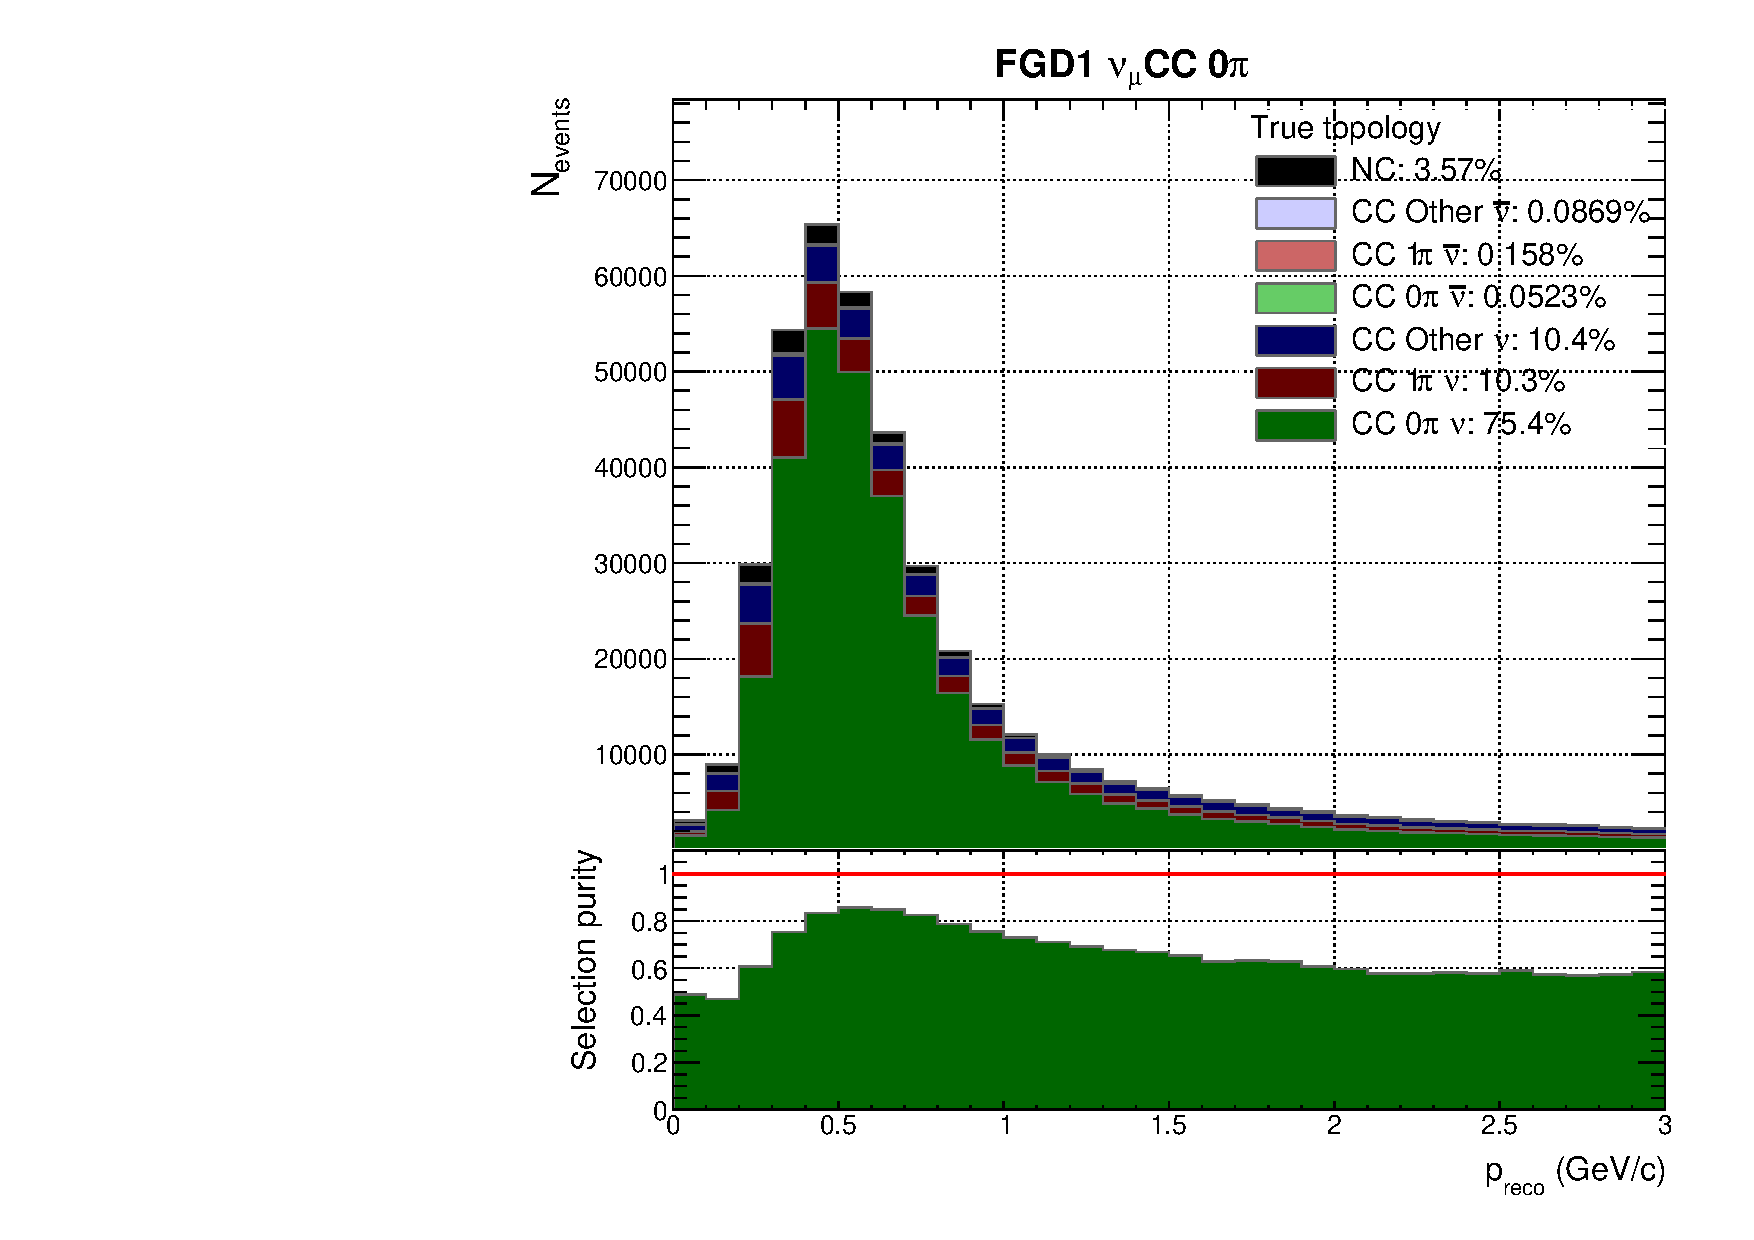
\includegraphics[width=\textwidth,page=1, trim={0mm 0mm 0mm 9mm}, clip]{figures/mach3/2018/Selection/2018_RedNDmatrix_rebin_verbose_may_noweights_diagnostics}
		\caption{Efficiency}
	\end{subfigure}
	\begin{subfigure}[t]{0.4\textwidth}
		\includegraphics[width=\textwidth,page=2, trim={0mm 0mm 0mm 9mm}, clip]{figures/mach3/2018/Selection/2018_RedNDmatrix_rebin_verbose_may_noweights_diagnostics}
		\caption{Purity}
	\end{subfigure}
\end{subfigure}

	\begin{subfigure}[t]{\textwidth}
		\centering
		\caption*{2017 analysis}
	\begin{subfigure}[t]{0.4\textwidth}
	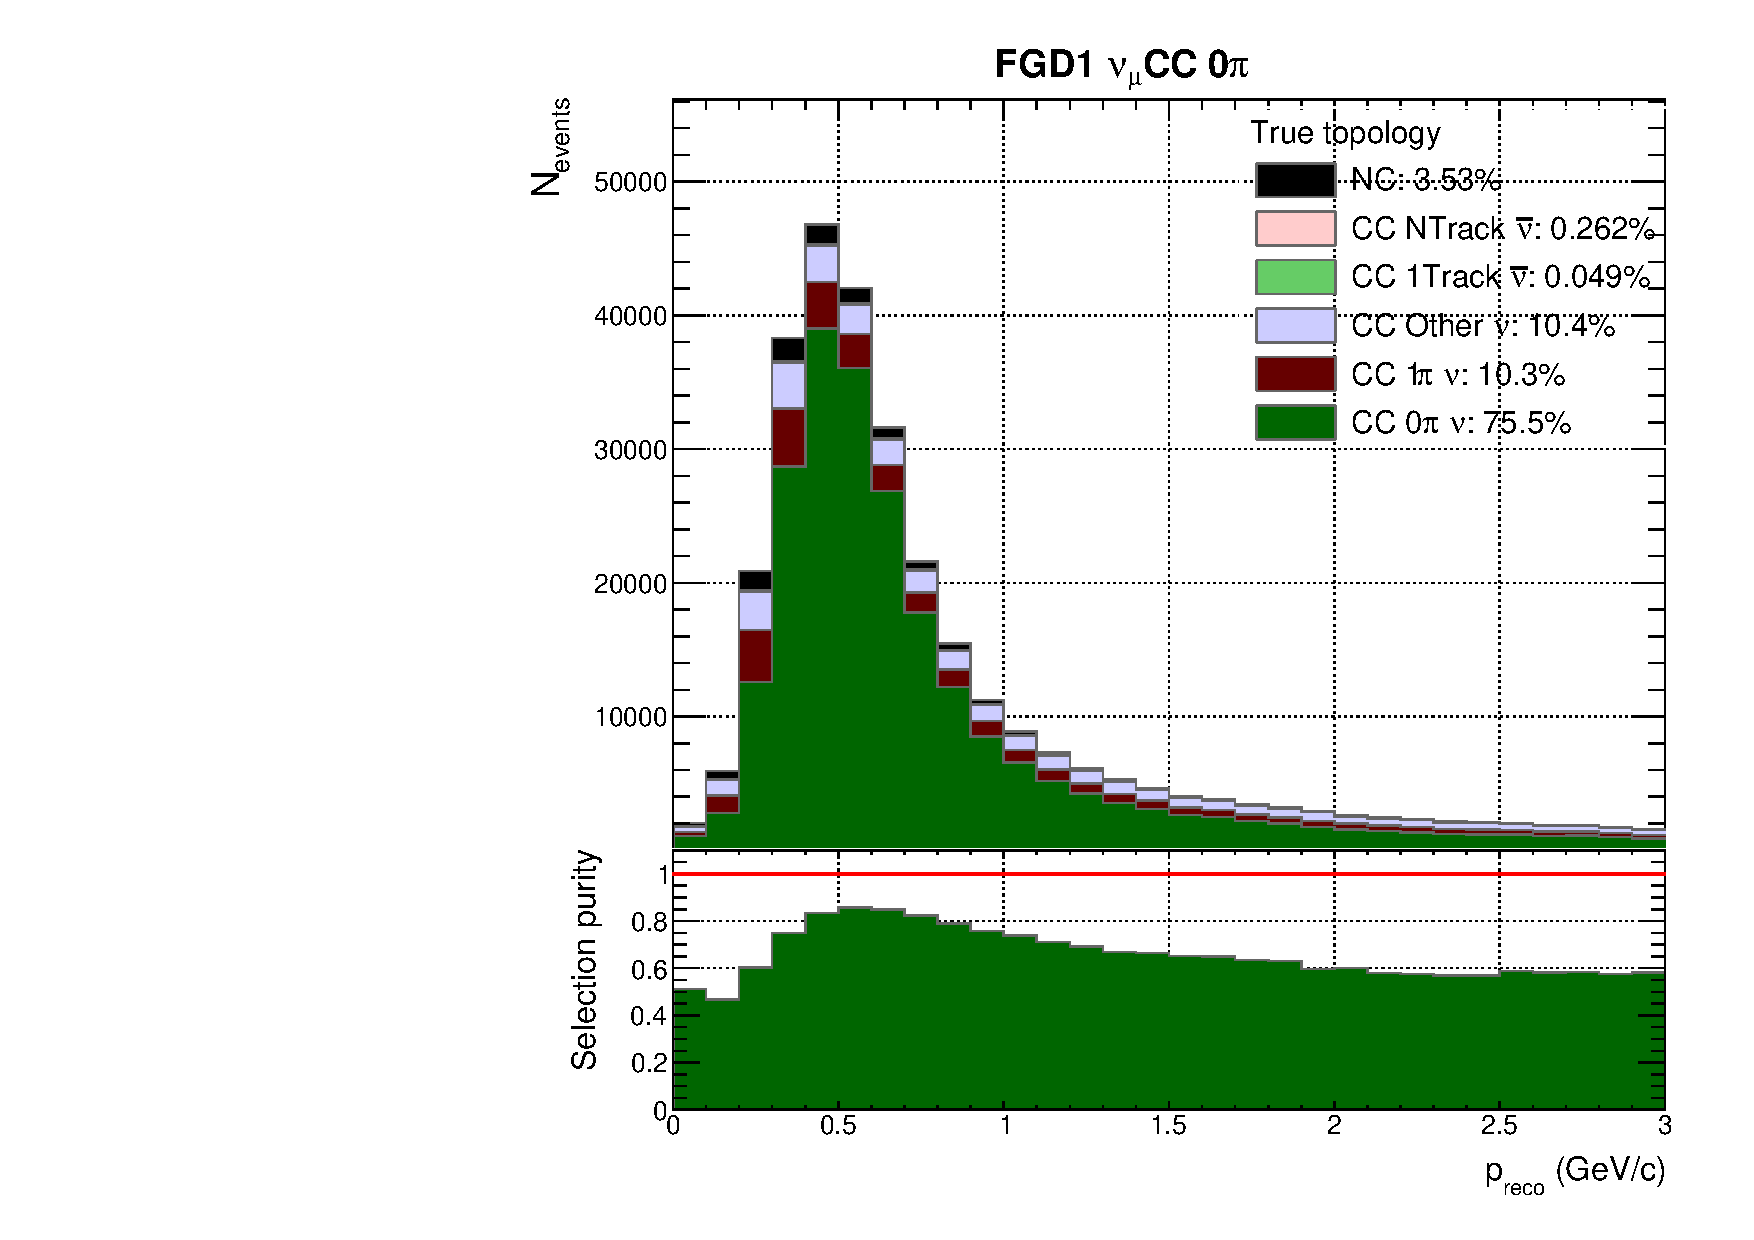
\includegraphics[width=\textwidth,page=1, trim={0mm 0mm 0mm 9mm}, clip]{figures/mach3/selection/2017b_Diag_WithSelection}
	\caption{Efficiency}
\end{subfigure}
\begin{subfigure}[t]{0.4\textwidth}
	\includegraphics[width=\textwidth,page=2, trim={0mm 0mm 0mm 9mm}, clip]{figures/mach3/selection/2017b_Diag_WithSelection}
	\caption{Purity}
\end{subfigure}
\end{subfigure}
\caption{FGD1 0$\pi$ efficiencies and purities for 2017 and 2018 analyses}
\label{fig:fgd1_cc0pi_eff_2017_2018}
\end{figure}

\subsection{\numubar in RHC}
The CC0$\pi$ RHC selections are much the same as the 2017 1Track selection, and as such the purity in \autoref{fig:numubar_cc0pi_topology_2018} is almost identical to \autoref{fig:ccnubar1trk_topology}. Both FGDs have similar purities and the largest contamination is right-sign single events in which the pion is missed, at about 9.5\%. The NC contribution is 5\% and the total wrong-sign contribution is $\sim5\%$, similar to the 1Trk selection. The difference comes primarily from the removed upper bound on the muon likelihood cut. Moving up in momentum, the purity reduces to about 60\% from 85\% at the event peak.
\begin{figure}[h]
	\begin{subfigure}[t]{0.49\textwidth}
		\includegraphics[width=\textwidth,page=13, trim={0mm 0mm 0mm 9mm}, clip]{figures/mach3/2018/Selection/2018_RedNDmatrix_rebin_verbose_may_noweights_diagnostics}
		\caption{FGD1}
	\end{subfigure}
	\begin{subfigure}[t]{0.49\textwidth}
		\includegraphics[width=\textwidth,page=19, trim={0mm 0mm 0mm 9mm}, clip]{figures/mach3/2018/Selection/2018_RedNDmatrix_rebin_verbose_may_noweights_diagnostics}
		\caption{FGD2}
	\end{subfigure}
	\caption{Breakdown of \numubar CC0$\pi$ selection events' true event topology for FGD1 and FGD2 }
	\label{fig:numubar_cc0pi_topology_2018}
\end{figure}

\autoref{fig:numubar_cc0pi_muon_2018} shows the muon tagging efficiency, which again is comparable to the 1Trk equivalent in \autoref{fig:ccnubar1trk_muon}. The largest mis-id comes from $\pi^+$ being reconstructed as the muon, and the wrong-sign contamination is small. At $\sim1.5\text{ GeV}$ we see the characteristic proton bump---which makes up 3\% of the total---in which the dE/dx of a proton is very similar to that of a muon, causing it to be the selected highest momentum positive track with a muon likelihood.
\begin{figure}[h]
	\begin{subfigure}[t]{0.49\textwidth}
		\includegraphics[width=\textwidth,page=14, trim={0mm 0mm 0mm 9mm}, clip]{figures/mach3/2018/Selection/2018_RedNDmatrix_rebin_verbose_may_noweights_diagnostics}
		\caption{FGD1}
	\end{subfigure}
	\begin{subfigure}[t]{0.49\textwidth}
		\includegraphics[width=\textwidth,page=20, trim={0mm 0mm 0mm 9mm}, clip]{figures/mach3/2018/Selection/2018_RedNDmatrix_rebin_verbose_may_noweights_diagnostics}
		\caption{FGD2}
	\end{subfigure}
	\caption{Breakdown of \numubar CC0$\pi$ selection events' true lepton candidate for FGD1 and FGD2}
	\label{fig:numubar_cc0pi_muon_2018}
\end{figure}

Moving to the 1$\pi$ \numubar selection, the purity is shown in \autoref{fig:numubar_cc1pi_topology_2018}. The \numubar RHC selection sees similar performance to the \numu FHC equivalent in \autoref{fig:cc1pi_topology}, reaching an overall purity of $50-54\%$, with FGD1 being the higher. The wrong-sign contamination is significant at 25-30\%, coming from a $\pi^+$ in a CC1$\pi^+$ or CC DIS event being reconstructed as the muon candidate, and the $\mu^-$ reconstructed as the $\pi^-$. The right-sign CCOther contamination is about 10\%, owing mostly to one or several missed $\pi$. We again see the CC0$\pi$ \numu peak at 1.5 GeV, where the proton (likely from a CCQE or 2p2h interaction) is reconstructed as the $\mu^+$.
\begin{figure}[h]
	\begin{subfigure}[t]{0.49\textwidth}
		\includegraphics[width=\textwidth,page=15, trim={0mm 0mm 0mm 9mm}, clip]{figures/mach3/2018/Selection/2018_RedNDmatrix_rebin_verbose_may_noweights_diagnostics}
		\caption{FGD1}
	\end{subfigure}
	\begin{subfigure}[t]{0.49\textwidth}
		\includegraphics[width=\textwidth,page=21, trim={0mm 0mm 0mm 9mm}, clip]{figures/mach3/2018/Selection/2018_RedNDmatrix_rebin_verbose_may_noweights_diagnostics}
		\caption{FGD2}
	\end{subfigure}
	\caption{Breakdown of \numubar CC1$\pi$ selection events' true event topology for FGD1 and FGD2 }
	\label{fig:numubar_cc1pi_topology_2018}
\end{figure}

\autoref{fig:numubar_cc1pi_muon_2018} shows the muon tagging efficiency, which in the event peak sits at 80\% and decreases to 50\% with increasing $p_{\text{reco}}$. Tagging the right-sign pion as the lepton candidate happens 20\% of the time, and protons at $p\sim1.5\text{ GeV}$ about 15\% of the time, making up a large fraction of mis-identification. However, the 1$\pi$ selection is still almost 10\% more efficient and pure than the old CCNTrack selection.
\begin{figure}[h]
	\begin{subfigure}[t]{0.49\textwidth}
		\includegraphics[width=\textwidth,page=16, trim={0mm 0mm 0mm 9mm}, clip]{figures/mach3/2018/Selection/2018_RedNDmatrix_rebin_verbose_may_noweights_diagnostics}
		\caption{FGD1}
	\end{subfigure}
	\begin{subfigure}[t]{0.49\textwidth}
		\includegraphics[width=\textwidth,page=22, trim={0mm 0mm 0mm 9mm}, clip]{figures/mach3/2018/Selection/2018_RedNDmatrix_rebin_verbose_may_noweights_diagnostics}
		\caption{FGD2}
	\end{subfigure}
	\caption{Breakdown of \numubar CC1$\pi$ selection events' true lepton candidate for FGD1 and FGD2}
	\label{fig:numubar_cc1pi_muon_2018}
\end{figure}

Finally \autoref{fig:numubar_ccOth_topology_2018} shows the purity of the \numubar CCOther selection, which collects all \numubar CC candidates that weren't classified as CC0$\pi$ or CC1$\pi$. As with the equivalent \numu selection, the sample suffers from low purity due to broken tracks and secondary interactions, leading to a mis-reconstructed number of pions in the event. The selection has an almost equal efficiency for \numubar CCOther events as it does for \numu CCOther events, and in FGD2 it's indeed more pure of wrong-sign events. It has a high NC contamination due to collecting high pion multiplicity events, causing a pion to be reconstructed as a muon in the TPC.  At low momentum, the purity is close to zero, being swamped by wrong-sign 0$\pi$ events in which the low momentum $\mu^-$ is identified as a $\mu^+$, owing to the changed likelihood cut which in the 2017 analysis was present to remove such events. The wrong-sign 0$\pi$ and 1$\pi$ contributions largely vanish above 500 MeV and the wrong sign component is almost exclusively \numu CCOther.
\begin{figure}[h]
	\begin{subfigure}[t]{0.49\textwidth}
		\includegraphics[width=\textwidth,page=17, trim={0mm 0mm 0mm 9mm}, clip]{figures/mach3/2018/Selection/2018_RedNDmatrix_rebin_verbose_may_noweights_diagnostics}
		\caption{FGD1}
	\end{subfigure}
	\begin{subfigure}[t]{0.49\textwidth}
		\includegraphics[width=\textwidth,page=23, trim={0mm 0mm 0mm 9mm}, clip]{figures/mach3/2018/Selection/2018_RedNDmatrix_rebin_verbose_may_noweights_diagnostics}
		\caption{FGD2}
	\end{subfigure}
	\caption{Breakdown of \numubar CCOther selection events' true event topology for FGD1 and FGD2 }
	\label{fig:numubar_ccOth_topology_2018}
\end{figure}

The muon tagging efficiency of the \numubar CCOther selection is shown in \autoref{fig:numubar_ccOth_muon_2018}, which echoes the conclusions above. The efficiency is below 50\% and has almost equal parts proton tagging and $\pi^+$ tagging as contaminants. The wrong sign tag happens primarily at low momentum, in which the charge is reconstructed in the magnetic field. The proton bump at 1.5 GeV is especially present in this selection.
\begin{figure}[h]
	\begin{subfigure}[t]{0.49\textwidth}
		\includegraphics[width=\textwidth,page=18, trim={0mm 0mm 0mm 9mm}, clip]{figures/mach3/2018/Selection/2018_RedNDmatrix_rebin_verbose_may_noweights_diagnostics}
		\caption{FGD1}
	\end{subfigure}
	\begin{subfigure}[t]{0.49\textwidth}
		\includegraphics[width=\textwidth,page=24, trim={0mm 0mm 0mm 9mm}, clip]{figures/mach3/2018/Selection/2018_RedNDmatrix_rebin_verbose_may_noweights_diagnostics}
		\caption{FGD2}
	\end{subfigure}
	\caption{Breakdown of \numubar CCOther selection events' true lepton candidate for FGD1 and FGD2}
	\label{fig:numubar_ccOth_muon_2018}
\end{figure}

\subsection{\numu in RHC}
As with the \numubar CC0$\pi$ selection, the \numu RHC CC0$\pi$ selection is largely identical to the 1Track equivalent in the 2017 analysis. The purity in \autoref{fig:numurhc_cc0pi_topology_2018} is above 53\%, with large contamination from right-sign 1$\pi$ and Other interactions, and the wrong-sign background making up 8\%, slightly less than the 1Track case. The NC contamination is almost identical to the 1Track selection at 9\%. We note the purity above 600 MeV stabilises at about 60\%.
\begin{figure}[h]
	\begin{subfigure}[t]{0.49\textwidth}
		\includegraphics[width=\textwidth,page=25, trim={0mm 0mm 0mm 9mm}, clip]{figures/mach3/2018/Selection/2018_RedNDmatrix_rebin_verbose_may_noweights_diagnostics}
		\caption{FGD1}
	\end{subfigure}
	\begin{subfigure}[t]{0.49\textwidth}
		\includegraphics[width=\textwidth,page=31, trim={0mm 0mm 0mm 9mm}, clip]{figures/mach3/2018/Selection/2018_RedNDmatrix_rebin_verbose_may_noweights_diagnostics}
		\caption{FGD2}
	\end{subfigure}
	\caption{Breakdown of \numu RHC CC0$\pi$ selection events' true event topology for FGD1 and FGD2 }
	\label{fig:numurhc_cc0pi_topology_2018}
\end{figure}

The muon tagging efficiency is shown in \autoref{fig:numurhc_cc0pi_muon_2018}, where we note 90\% above 1 GeV. At the event peak the efficiency sits at 55\%, leading to overall 78\%. In and below the event peak the main contamination is from $\pi^-$ (13\%) and as we go down in momentum the wrong-sign contributions increase due to wrongly reconstructing the charge in the magnet. At low momentum the wrong-sign component is $\times10$ larger than the right-sign.
\begin{figure}[h]
	\begin{subfigure}[t]{0.49\textwidth}
		\includegraphics[width=\textwidth,page=26, trim={0mm 0mm 0mm 9mm}, clip]{figures/mach3/2018/Selection/2018_RedNDmatrix_rebin_verbose_may_noweights_diagnostics}
		\caption{FGD1}
	\end{subfigure}
	\begin{subfigure}[t]{0.49\textwidth}
		\includegraphics[width=\textwidth,page=32, trim={0mm 0mm 0mm 9mm}, clip]{figures/mach3/2018/Selection/2018_RedNDmatrix_rebin_verbose_may_noweights_diagnostics}
		\caption{FGD2}
	\end{subfigure}
	\caption{Breakdown of \numu RHC CC0$\pi$ selection events' true lepton candidate for FGD1 and FGD2}
	\label{fig:numurhc_cc0pi_muon_2018}
\end{figure}

The CC1$\pi$ purity is shown in \autoref{fig:numurhc_cc1pi_topology_2018}, where we again see a large wrong-sign contribution at low momentum, primarily from \numubar 1$\pi$ events. The purity is 43\% overall, and a meagre 20\% in the event peak. The right-sign CCOther amount is constant with momentum, making up almost 1/3 at higher momentum.
\begin{figure}[h]
	\begin{subfigure}[t]{0.49\textwidth}
		\includegraphics[width=\textwidth,page=27, trim={0mm 0mm 0mm 9mm}, clip]{figures/mach3/2018/Selection/2018_RedNDmatrix_rebin_verbose_may_noweights_diagnostics}
		\caption{FGD1}
	\end{subfigure}
	\begin{subfigure}[t]{0.49\textwidth}
		\includegraphics[width=\textwidth,page=33, trim={0mm 0mm 0mm 9mm}, clip]{figures/mach3/2018/Selection/2018_RedNDmatrix_rebin_verbose_may_noweights_diagnostics}
		\caption{FGD2}
	\end{subfigure}
	\caption{Breakdown of \numu RHC CC1$\pi$ selection events' true event topology for FGD1 and FGD2 }
	\label{fig:numurhc_cc1pi_topology_2018}
\end{figure}

The muon tagging efficiency in \autoref{fig:numurhc_cc1pi_muon_2018} performs similarly to the NTrack selection at 65\%. At the event peak the efficiency is barely 20\%--the rest split almost equally amongst $\pi^-$, $\pi^+$ and $\mu^+$---but increases steadily to 85\% at higher momentum, where to wrong-sign component vanishes. The total wrong-sign contribution is 12\% but is dominant at low momentum. The $\pi^-$ contribution is sizeable at 22\%, which dies off at higher momentum.
\begin{figure}[h]
	\begin{subfigure}[t]{0.49\textwidth}
		\includegraphics[width=\textwidth,page=28, trim={0mm 0mm 0mm 9mm}, clip]{figures/mach3/2018/Selection/2018_RedNDmatrix_rebin_verbose_may_noweights_diagnostics}
		\caption{FGD1}
	\end{subfigure}
	\begin{subfigure}[t]{0.49\textwidth}
		\includegraphics[width=\textwidth,page=34, trim={0mm 0mm 0mm 9mm}, clip]{figures/mach3/2018/Selection/2018_RedNDmatrix_rebin_verbose_may_noweights_diagnostics}
		\caption{FGD2}
	\end{subfigure}
	\caption{Breakdown of \numu RHC CC1$\pi$ selection events' true lepton candidate for FGD1 and FGD2}
	\label{fig:numurhc_cc1pi_muon_2018}
\end{figure}

The \numu RHC CCOther selection's purity seen in \autoref{fig:numurhc_ccOth_topology_2018} is relatively high compared to other CC Other selection; overall 61\%. At low momentum the NC contribution is the largest, which is also the largest background overall at 13\%. Interestingly, the right-sign 0$\pi$ selection contaminates the sample 10\% and is the second largest contamination. Since the sign selection looks for a negative track for \numu selections, the CC0$\pi$ contribution can not come from a proton track being the muon candidate, and must be broken tracks being reconstructed as multiple pions.
\begin{figure}[h]
	\begin{subfigure}[t]{0.49\textwidth}
		\includegraphics[width=\textwidth,page=29, trim={0mm 0mm 0mm 9mm}, clip]{figures/mach3/2018/Selection/2018_RedNDmatrix_rebin_verbose_may_noweights_diagnostics}
		\caption{FGD1}
	\end{subfigure}
	\begin{subfigure}[t]{0.49\textwidth}
		\includegraphics[width=\textwidth,page=35, trim={0mm 0mm 0mm 9mm}, clip]{figures/mach3/2018/Selection/2018_RedNDmatrix_rebin_verbose_may_noweights_diagnostics}
		\caption{FGD2}
	\end{subfigure}
	\caption{Breakdown of \numu RHC CCOther selection events' true event topology for FGD1 and FGD2 }
	\label{fig:numurhc_ccOth_topology_2018}
\end{figure}

The corresponding muon efficiency is shown in \autoref{fig:numurhc_ccOth_muon_2018}, where we see close to zero efficiency at low momentum. In this region the electron is the principal muon candidate, but dies down above 200 MeV. After that the $\pi^-$ is the only competing background at $\sim20\%$. The overall efficiency is 68\% and stabilises at 1 GeV, coinciding with the event distribution peak.
\begin{figure}[h]
	\begin{subfigure}[t]{0.49\textwidth}
		\includegraphics[width=\textwidth,page=30, trim={0mm 0mm 0mm 9mm}, clip]{figures/mach3/2018/Selection/2018_RedNDmatrix_rebin_verbose_may_noweights_diagnostics}
		\caption{FGD1}
	\end{subfigure}
	\begin{subfigure}[t]{0.49\textwidth}
		\includegraphics[width=\textwidth,page=36, trim={0mm 0mm 0mm 9mm}, clip]{figures/mach3/2018/Selection/2018_RedNDmatrix_rebin_verbose_may_noweights_diagnostics}
		\caption{FGD2}
	\end{subfigure}
	\caption{Breakdown of \numu RHC CCOther selection events' true lepton candidate for FGD1 and FGD2}
	\label{fig:numurhc_ccOth_muon_2018}
\end{figure}

A summary of the 2018 analysis' selection efficiencies and purities is shown in \autoref{tab:eff_pur_summary_2018}.
\begin{table}[h]
	\centering
	\begin{tabular}{ l | c c }
		\hline
		\hline
		Selection 					   & Efficiency (\%) & Purity (\%) \\ 
		\hline
		\FGDCCNoPi{1}{\numu}           & 93.7  & 75.4  \\% \hline
		\FGDCCNoPi{2}{\numu}           & 93.0  & 73.3  \\% \hline
		\hline
		\FGDCCOnePi{1}{\numu}          & 83.4  & 57.3  \\% \hline
		\FGDCCOnePi{2}{\numu}          & 83.0  & 56.7  \\% \hline
		\hline
		\FGDCCOther{1}{\numu}          & 73.0  & 64.9  \\% \hline
		\FGDCCOther{2}{\numu}          & 73.4  & 64.9  \\% \hline
		\hline
		\FGDCCNoPi{1}{\numubar}           & 89.4  & 75.2  \\% \hline
		\FGDCCNoPi{2}{\numubar}           & 87.8  & 74.0  \\% \hline
		\hline
		\FGDCCOnePi{1}{\numubar}          & 65.0  & 53.5  \\% \hline
		\FGDCCOnePi{2}{\numubar}          & 61.0  & 49.6  \\% \hline
		\hline
		\FGDCCOther{1}{\numubar}          & 44.1  & 24.6  \\% \hline
		\FGDCCOther{2}{\numubar}          & 41.6  & 23.6  \\% \hline
		\hline		
		\FGDCCNoPi{1}{\numu RHC}           & 79.7  & 55.6  \\% \hline
		\FGDCCNoPi{2}{\numu RHC}           & 77.8  & 53.0 \\% \hline
		\hline
		\FGDCCOnePi{1}{\numu RHC}          & 65.7  & 43.4  \\% \hline
		\FGDCCOnePi{2}{\numu RHC}          & 66.8  & 43.1  \\% \hline
		\hline
		\FGDCCOther{1}{\numu RHC}          & 68.8  & 61.0  \\% \hline
		\FGDCCOther{2}{\numu RHC}          & 69.0  & 60.8  \\% \hline
		\hline
		\hline
	\end{tabular}
	\caption{Efficiency and purity summary for all selections with the range $0 < p_{reco} < 3\text{ GeV/c}$, directly comparable to \autoref{tab:eff_pur_summary}}
	\label{tab:eff_pur_summary_2018}
\end{table}

\section{Binning the Selections}
With the large increase in statistics from using run 7 and 8 data, a re-binning of the two reconstructed event observables \pmu and \cosmu is due. As was the case in \autoref{sec:binning_2017}, we base the binning on requiring $\sim20$ raw MC events per bin, which is roughly equivalent to 1-2 data events. We keep in mind the approximate momentum resolution of ND280 is $\sim50\text{ MeV}$ and the angular resolution $\sim2\degree$.

Here we re-bin all selections for 2018 analysis using the above criteria, leading to a drastic increase in the number of bins from the 2017 analysis, which was 1624. The total number of bins is now 4238, of which 2942 are FHC (six selections) and 1188 are RHC (12 selections). We note the FGD1 and 2 CC0$\pi$ binning alone (1682) is more bins than was present in total for 2017 (1624).

\begin{itemize}
	\item FGD1+2 CC0$\pi$: 841 fit bins\\
	$p_\mu$ (MeV/c) = 0, 200, 300, 400, 450, 500, 550, 600, 650, 700, 750, 800, 850, 900, 950, 1000, 1050, 1100, 1200, 1300, 1400, 1500, 1600, 1700, 1800, 2000, 2500, 3000, 5000, 30000.\\
	$\cos\theta_\mu$ = -1, 0.5, 0.6, 0.7, 0.76, 0.78, 0.8, 0.83, 0.85, 0.88, 0.89, 0.9, 0.91, 0.92, 0.925, 0.93, 0.935, 0.94, 0.945, 0.95, 0.955, 0.96, 0.965, 0.97, 0.975, 0.98, 0.985, 0.99, 0.995, 1.
	
	\item FGD1+2 CC1$\pi$: 288 fit bins\\
	$p_\mu$ (MeV/c) = 0, 300, 350, 400, 500, 600, 650, 700, 750, 800, 900, 1000, 1100, 1200, 1500, 2000, 3000, 5000, 30000.\\
	$\cos\theta_\mu$ = -1, 0.6, 0.7, 0.8, 0.85, 0.88, 0.9, 0.92, 0.93, 0.94, 0.95, 0.96, 0.97, 0.98, 0.99, 0.995, 1.
	
	\item FGD1+2 CCOther: 342 fit bins\\
	$p_\mu$ (MeV/c) = 0, 300, 400, 500, 600, 650, 700, 750, 800, 900, 1000, 1100, 1250, 1500, 1750, 2000, 3000, 5000, 30000.\\
	$\cos\theta_\mu$ = -1, 0.6, 0.7, 0.76, 0.8, 0.85, 0.88, 0.89, 0.9, 0.91, 0.92, 0.93, 0.94, 0.95, 0.96, 0.97, 0.98, 0.99, 0.995, 1.
	
	\item FGD1+2 CC0$\pi$ RHC: 306 fit bins\\
	$p_\mu$ (MeV/c) = 0, 300, 400, 500, 550, 600, 650, 700, 750, 800, 900, 1000, 1100, 1200, 1500, 2000, 4000, 30000.\\
	$\cos\theta_\mu$ = -1, 0.6, 0.7, 0.8, 0.85, 0.9, 0.92, 0.93, 0.94, 0.95, 0.96, 0.965, 0.97, 0.975, 0.98, 0.985, 0.99, 0.995, 1.
	
	\item FGD1+2 CC1$\pi$ RHC: 48 fit bins \\
	$p_\mu$ (MeV/c) = 0, 500, 700, 900, 1300, 2500, 30000.\\
	$\cos\theta_\mu$ = -1, 0.7, 0.8, 0.9, 0.94, 0.96, 0.98, 0.99, 1
	
	\item FGD1+2 CCOther RHC: 80 fit bins \\
	$p_\mu$ (MeV/c) = 0, 600, 800, 1000, 1250, 1500, 2000, 4000, 30000.\\
	$\cos\theta_\mu$ = -1, 0.7, 0.8, 0.85, 0.9, 0.93, 0.95, 0.97, 0.98, 0.99, 1.
	
	\item FGD1+2 CC0$\pi$ $\nu$ RHC: 120 fit bins \\
	$p_\mu$ (MeV/c) = 0, 300, 500, 700, 800, 900, 1250, 1500, 2000, 4000, 30000.\\
	$\cos\theta_\mu$ = -1, 0.7, 0.8, 0.85, 0.88, 0.9, 0.92, 0.94, 0.96, 0.97, 0.98, 0.99, 1.
	
	\item FGD1+2 CC1$\pi$ $\nu$ RHC: 40 fit bins \\
	$p_\mu$ (MeV/c) = 0, 600, 800, 1500, 30000.\\
	$\cos\theta_\mu$ = -1, 0.7, 0.8, 0.86, 0.9, 0.94, 0.96, 0.97, 0.98, 0.99, 1
	
	\item FGD1+2 CCOther $\nu$ RHC: 54 fit bins \\
	$p_\mu$ (MeV/c) = 0, 600, 1000, 1250, 2000, 4000, 30000.\\
	$\cos\theta_\mu$ = -1, 0.7, 0.8, 0.86, 0.9, 0.93, 0.95, 0.97, 0.99, 1.
\end{itemize}

\section{Systematics}
\label{sec:syst_2018}
The 2018 iteration of the fits to ND280 data was intended primarily a statistics update, including run 7 and 8 data, and a suitable update to the RHC selections to match the FHC selections. There was therefore comparably few updates to the treatment of systematics.

\subsection{The Beamline and Neutrino Flux}
The flux systematics saw no change and follows that prescribed in \autoref{subsec:syst_flux}.

\subsection{The ND280 Detector}
The systematics in \autoref{subsec:syst_nd280} are used again in the 2018 analysis. 

One more systematic was added to the detector response: the proton secondary interaction systematic. It is analogous to the pion secondary interaction but applies to protons instead, so allows proton tracks to be modified in the reconstruction. Since the proton ID is excellent when $p < 1.4\text{ GeV}$, this systematic is only important for anti-neutrino selections with $p > 1.4\text{ GeV}$, where there is a risk of the proton being assigned as the lepton candidate.

The parameterisation of the systematics is also unchanged to \autoref{subsec:syst_nd280}---we assign correlated normalisation parameters to each \pmu, \cosmu, merging similar responses when possible. Since the number of selections increased from 14 to 18 and the number of bins increased from 1624 to 4238, a new ND280 covariance matrix had to be generated. However, the number of bins increase by $\sim2.6$, and making the equivalent increase in detector parameters would bring the number of ND280 parameters to $\sim1500$, so a more aggressive bin merging was applied. The parameterisation of ND280 with identical binning to the fit binning (so 4238 ND280 parameters) was also tested and is presented throughout as a reference.

The bin merging was approached in two ways: bins were merged if 1) there was a <5\% difference in effect from ND280 systematics, or 2) the effect of the systematics was <5\% and the bin content was less than one and the effect of the systematics on the bin was to change the number of events by less than one. This bin merging strategy is intended to merge bins with low response to the ND280 systematics and bins of low statistics. 

The number of final ND280 detector parameters decreased from 4238 to 1076 and favours finer binning for the high statistics FHC selections, as intended. The binning was as follows:
\begin{itemize}
	\item FGD1 and FGD2 CC0$\pi$: 272 detector bins (841) \\
	$p_\mu$ (GeV/c): 0, 200, 300, 400, 450, 550, 600, 650, 700, 750, 800, 850, 900, 950, 1000, 1400, 5000, 30000\\
	$\cos\theta_\mu$: -1, 0.5, 0.6, 0.7, 0.76, 0.8, 0.83, 0.85, 0.88, 0.965, 0.97, 0.975, 0.98, 0.985, 0.99, 0.995, 1
	
	\item FGD1 and FGD2 CC1$\pi$: 110 detector bins (288) \\
	$p_\mu$ (GeV/c): 0, 300, 350, 400, 500, 600, 650, 700, 1100, 3000, 5000, 30000\\
	$\cos\theta_\mu$: -1, 0.6, 0.7, 0.8, 0.85, 0.88, 0.9, 0.92, 0.93, 0.94, 1
	
	\item FGD1 and FGD2 CCOther: 72 detector bins (342) \\
	$p_\mu$ (GeV/c): 0, 300, 400, 600, 650, 1750, 2000, 5000, 30000\\
	$\cos\theta_\mu$: -1, 0.6, 0.93, 0.94, 0.95, 0.96, 0.98, 0.99, 0.995, 1
	
	\item FGD1 and FGD2 CC0$\pi$ RHC: 49 detector bins (306) \\
	$p_\mu$ (GeV/c): 0, 300, 400, 500, 550, 2000, 4000, 30000\\
	$\cos\theta_\mu$: -1, 0.6, 0.7, 0.8, 0.85, 0.9, 0.96, 1 
	
	\item FGD1 and FGD2 CC1$\pi$ RHC: 4 detector bins (48) \\
	$p_\mu$ (GeV/c): 0, 500, 30000.\\
	$\cos\theta_\mu$: -1, 0.7, 1
	
	\item FGD1 and FGD2 CCOther RHC: 6 detector bins (80) \\
	$p_\mu$ (GeV/c): 0, 600, 800, 30000.\\
	$\cos\theta_\mu$: -1, 0.7, 1.
	
	\item FGD1 and FGD2 CC0$\pi$ RHC $\nu$: 15 detector bins (120) \\
	$p_\mu$ (GeV/c): 0, 300, 500, 700, 800, 30000.\\
	$\cos\theta_\mu$: -1, 0.7, 0.8, 1.
	
	\item FGD1 and FGD2 CC1$\pi$ RHC $\nu$: 6 detector bins (40) \\
	$p_\mu$ (GeV/c): 0, 600, 800, 30000.\\
	$\cos\theta_\mu$: -1, 0.7, 1
	
	\item FGD1 and FGD2 CCOther RHC $\nu$: 4 detector bins (54)\\
	$p_\mu$ (GeV/c): 0, 600, 30000.\\
	$\cos\theta_\mu$: -1, 0.7, 1.
\end{itemize}

The $\chi^2/\text{nbins}$ for each bin's content when fitting a Gaussian is shown in \autoref{fig:det_chi2_ndof}. There are some clear outliers which follow a repeating pattern: this is the lowest momentum bin which often has bimodal distributions due to pions entering and exciting the selection from variation systematics. In most cases the difference in the $\sigma$ between the distribution and the fitted Gaussian is < 0.1 events, although modelling the distribution as a Gaussian is not ideal.
\begin{figure}[h]
	\begin{subfigure}[t]{0.7\textwidth}
		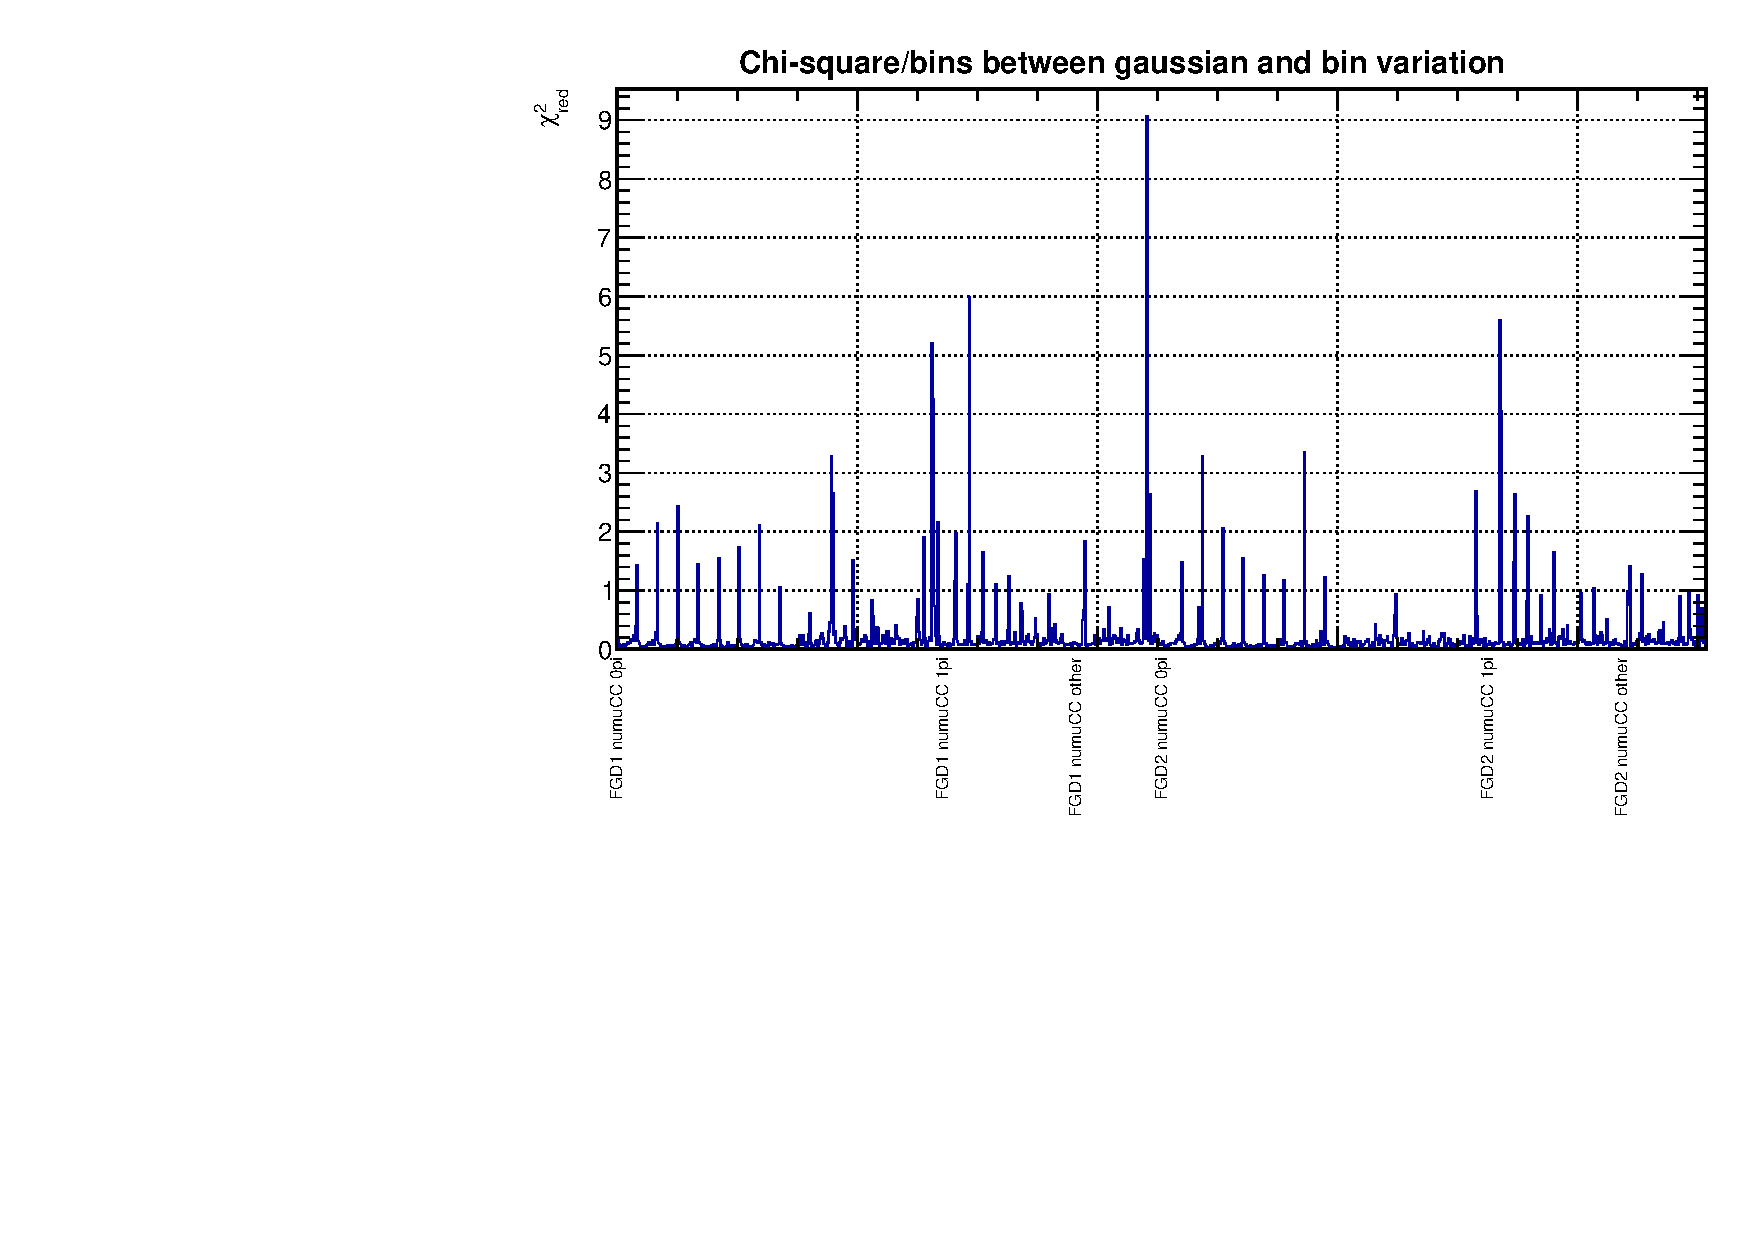
\includegraphics[width=\textwidth,page=1, trim={0mm 0mm 0mm 0mm}, clip]{figures/det/fhc_v7_chi2ndof}
		\caption{FHC}
	\end{subfigure}

	\begin{subfigure}[t]{0.7\textwidth}
		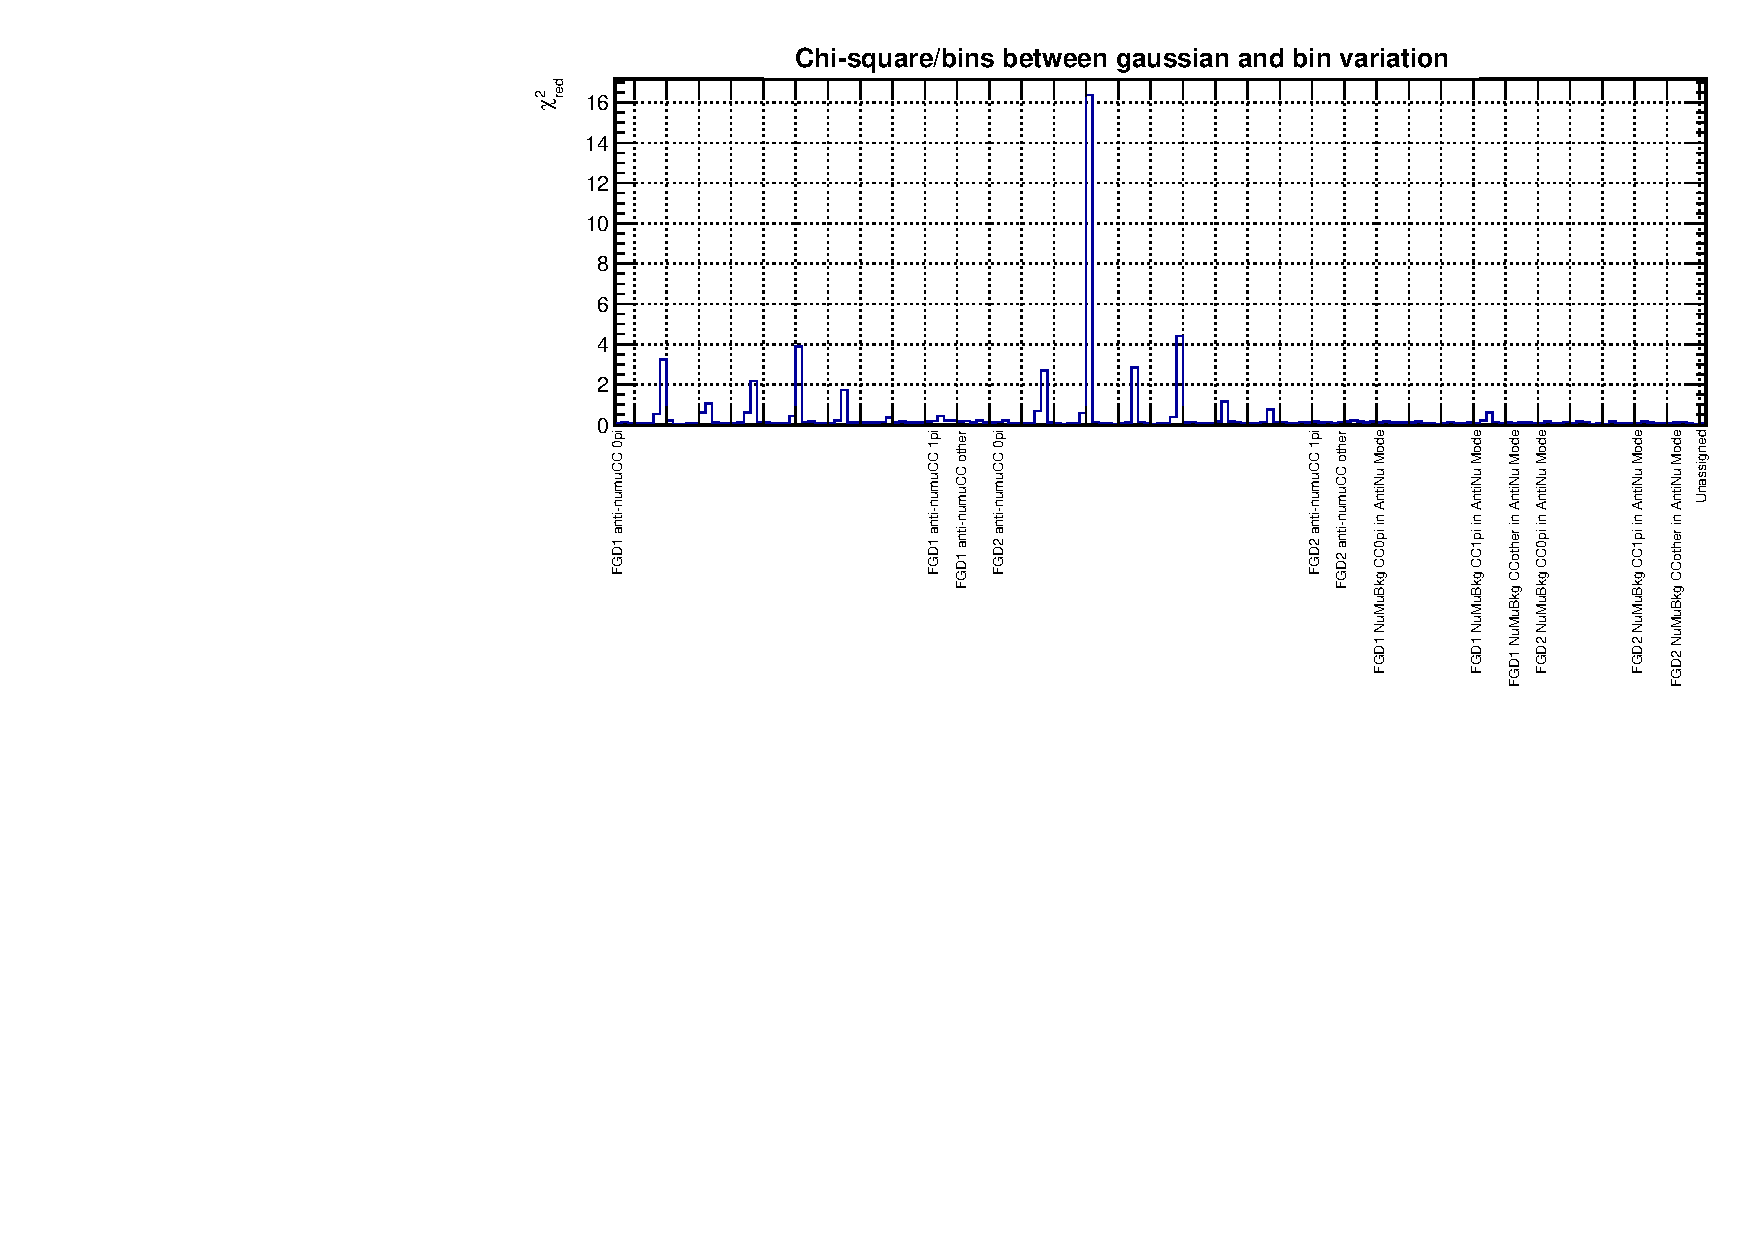
\includegraphics[width=\textwidth,page=1, trim={0mm 0mm 0mm 0mm}, clip]{figures/det/rhc_v7_chi2ndof}
		\caption{RHC}
	\end{subfigure}
\caption{$\chi^2/\text{nbins}$ for the reduced detector covariance matrix bins when fitting the bin's content distribution to a Gaussian}
\label{fig:det_chi2_ndof}
\end{figure}

\autoref{fig:det_binbybin} shows the event distributions for the three worst bins in \autoref{fig:det_chi2_ndof} (upper panel), which are all bimodal. We note all these cases to be low statistics (x-axis) so in reality have a low overall impact on the fit. The bottom panel shows a random selection of other bins which are better behaved.
\begin{figure}[h]
	\begin{subfigure}[t]{0.32\textwidth}
		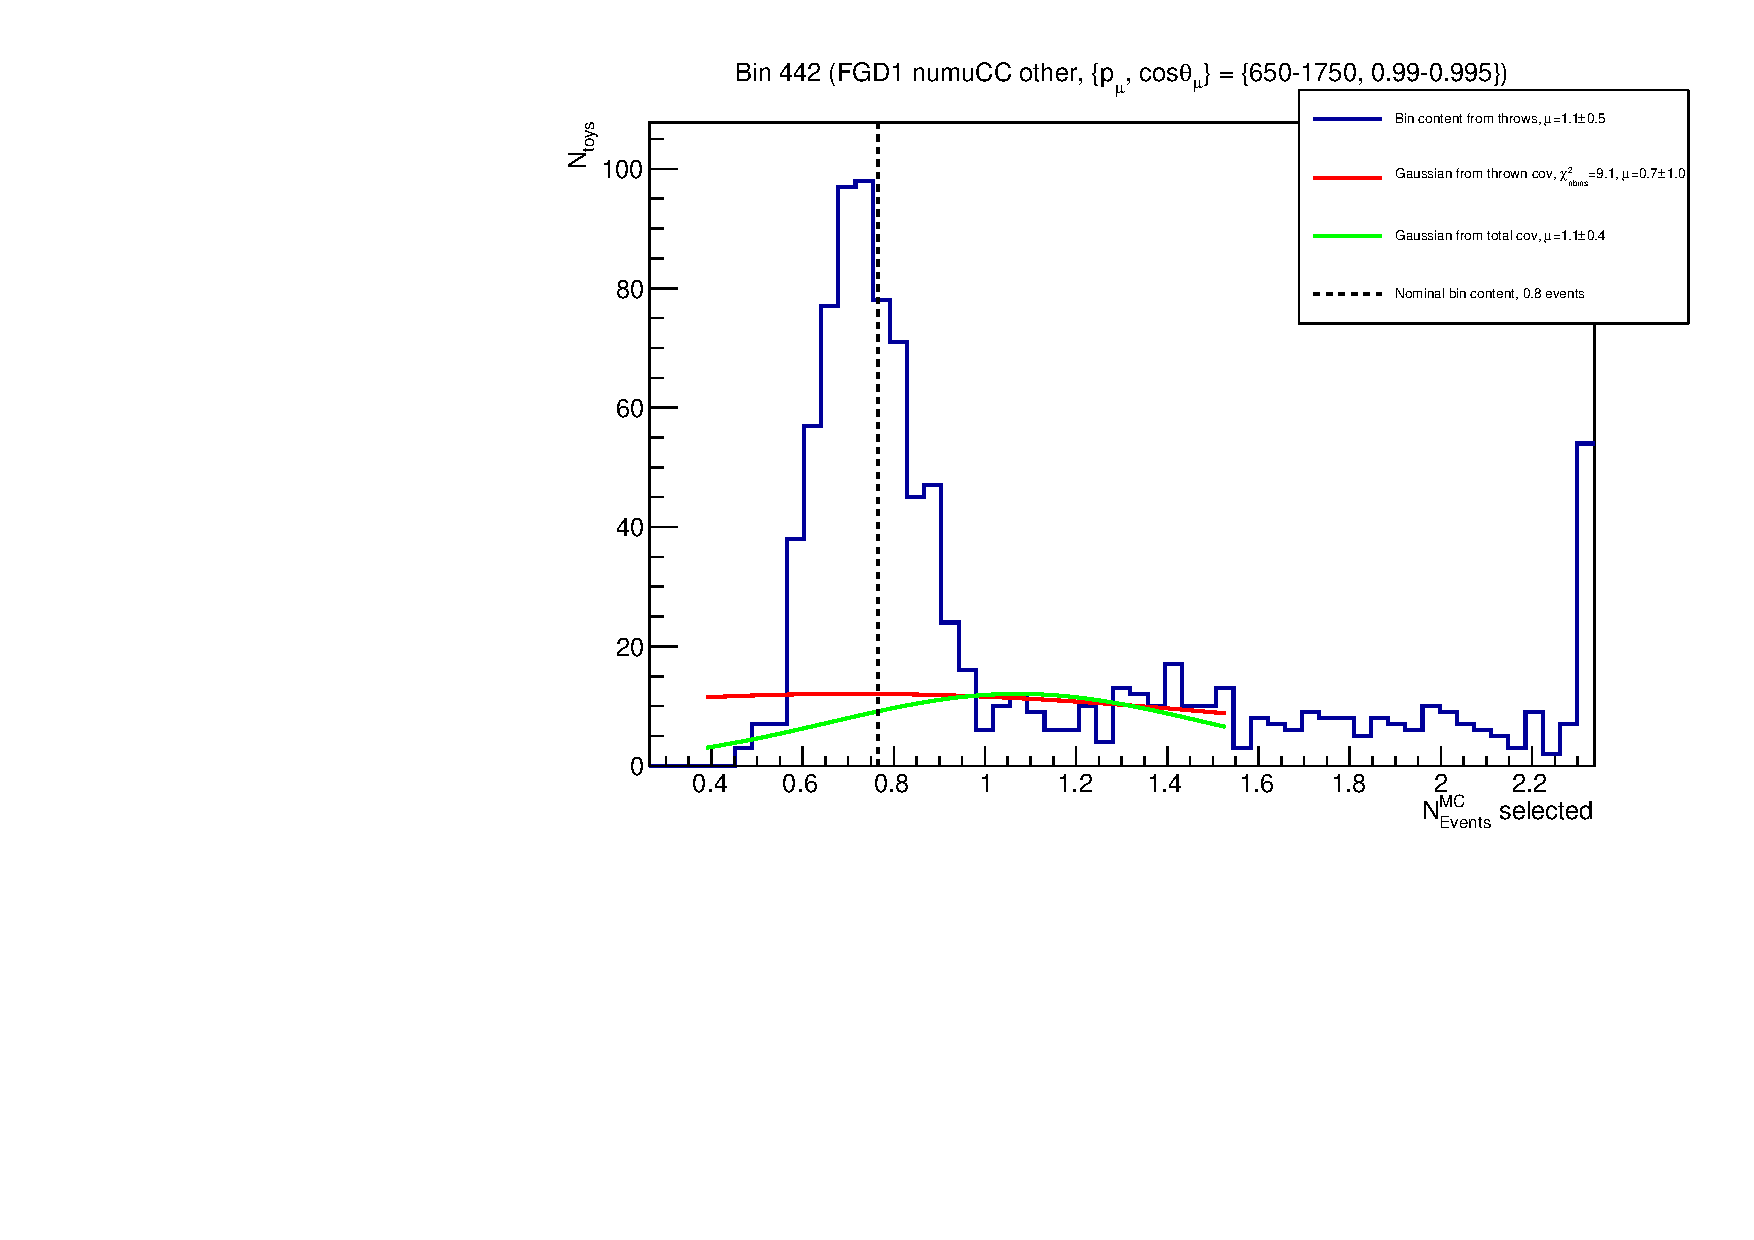
\includegraphics[width=\textwidth,page=1, trim={0mm 0mm 0mm 0mm}, clip]{figures/det/fdg1_numu_ccoth_bad}
	\end{subfigure}
	\begin{subfigure}[t]{0.32\textwidth}
		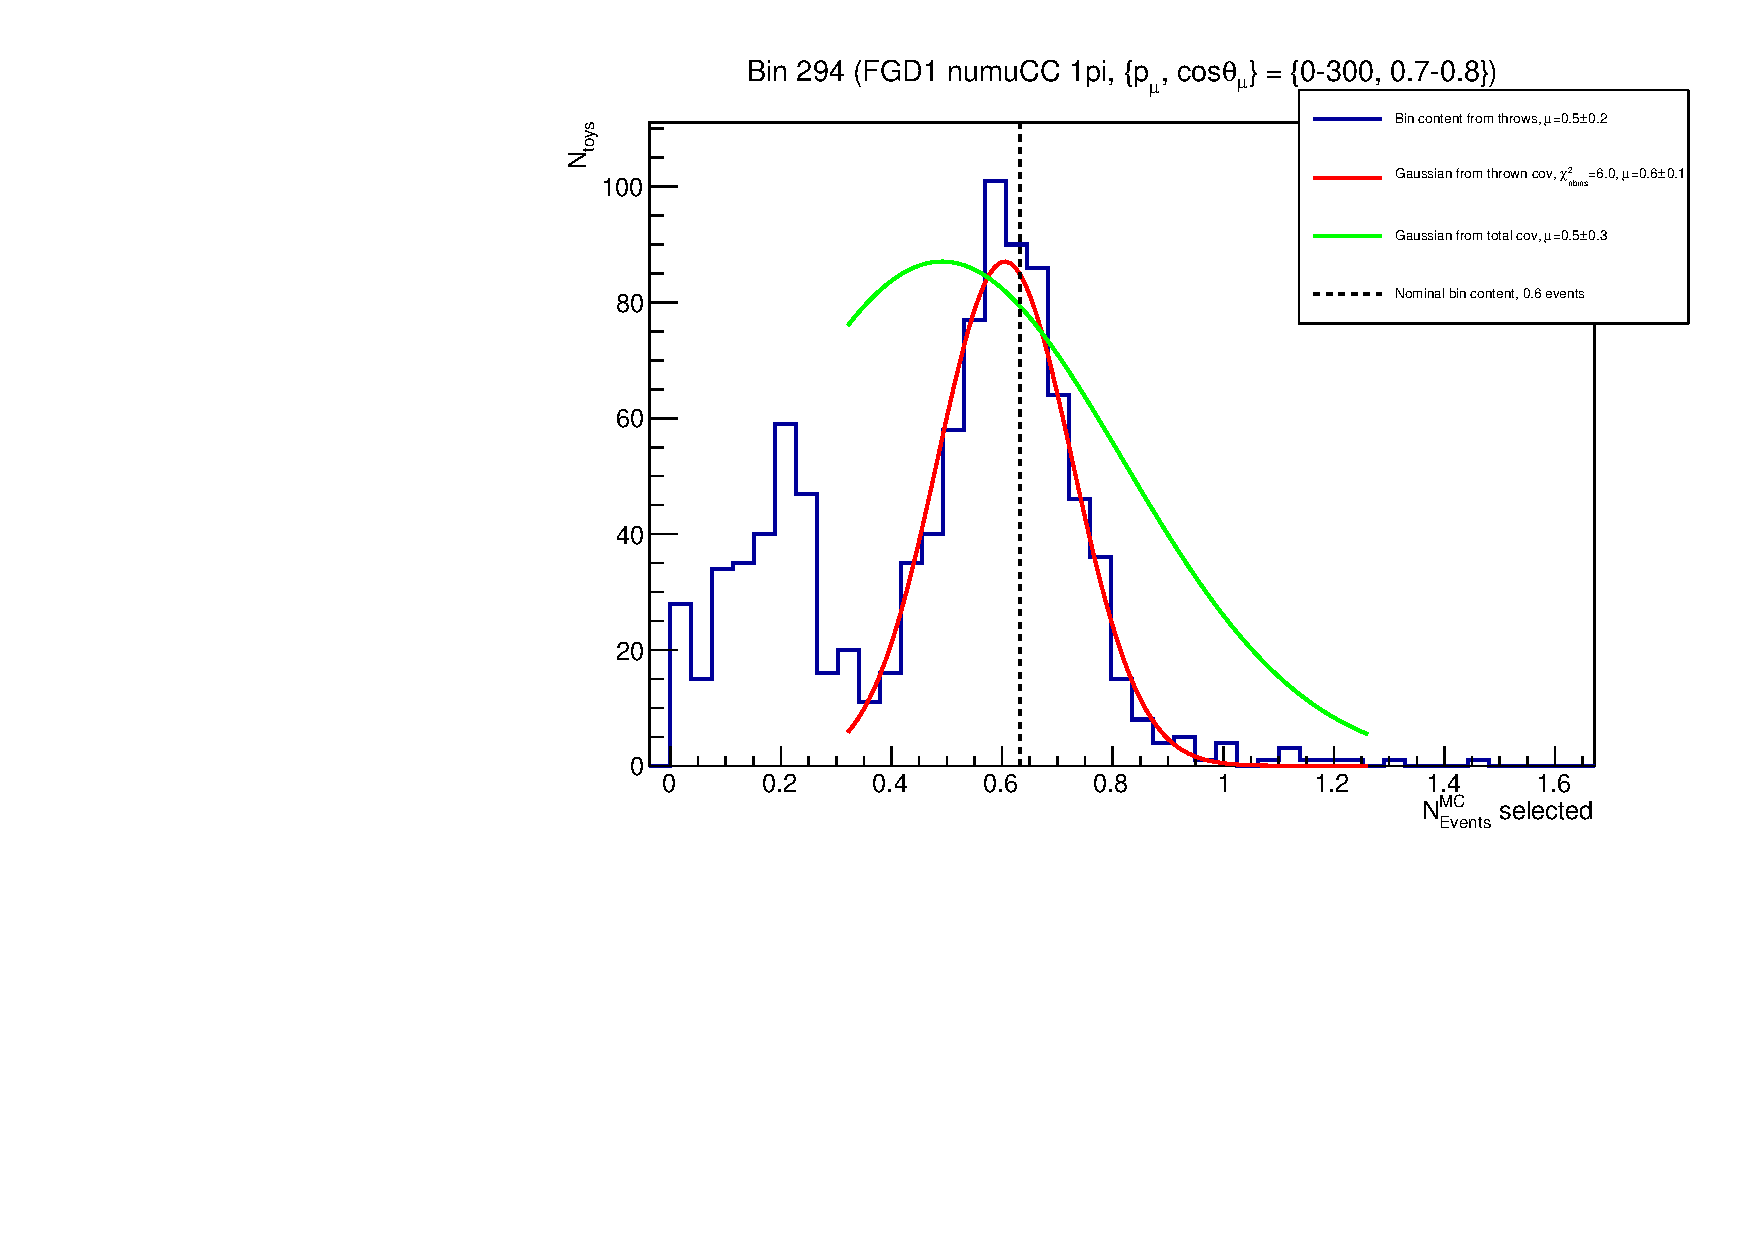
\includegraphics[width=\textwidth,page=1, trim={0mm 0mm 0mm 0mm}, clip]{figures/det/fgd1_numu_1pi_bad}
	\end{subfigure}
	\begin{subfigure}[t]{0.32\textwidth}
		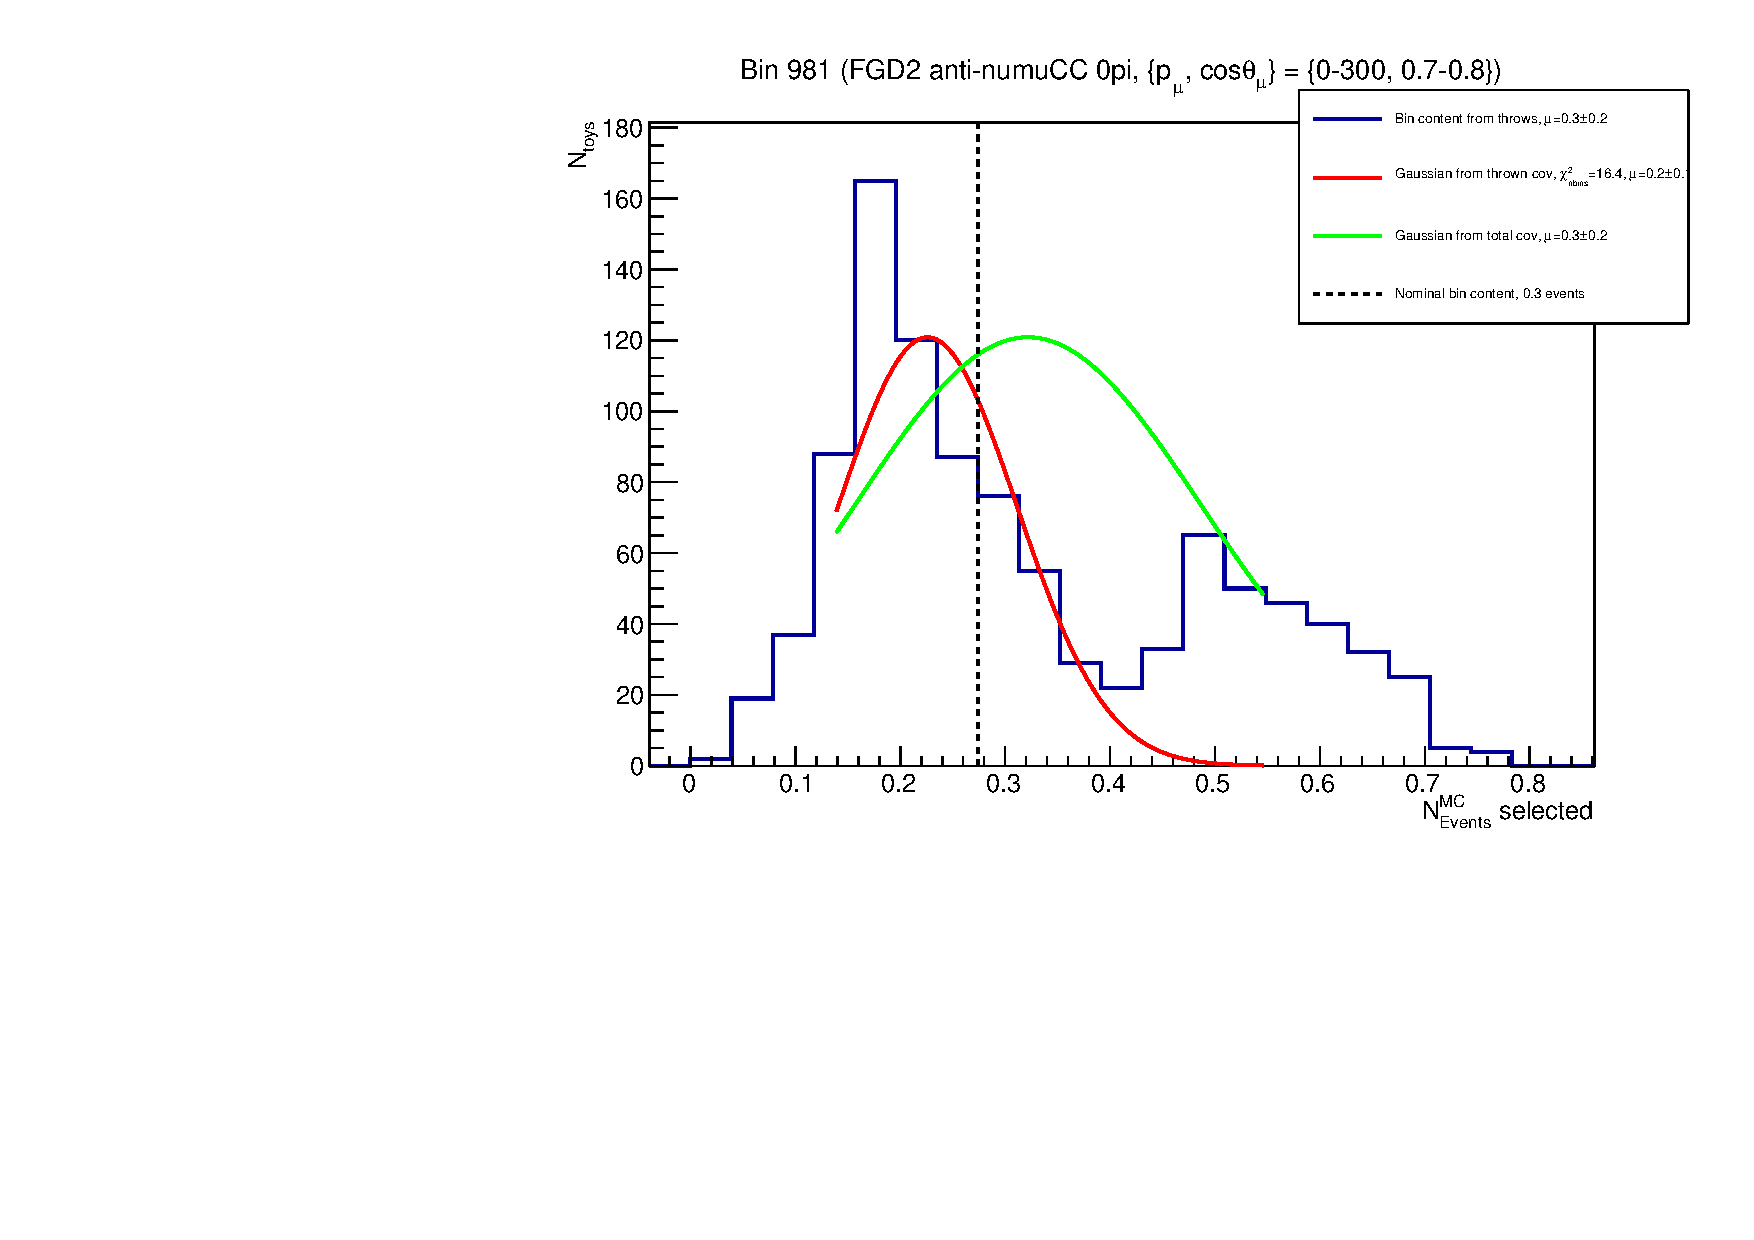
\includegraphics[width=\textwidth,page=1, trim={0mm 0mm 0mm 0mm}, clip]{figures/det/fgd2_numubar_0pi_bad}
	\end{subfigure}

	\begin{subfigure}[t]{0.32\textwidth}
		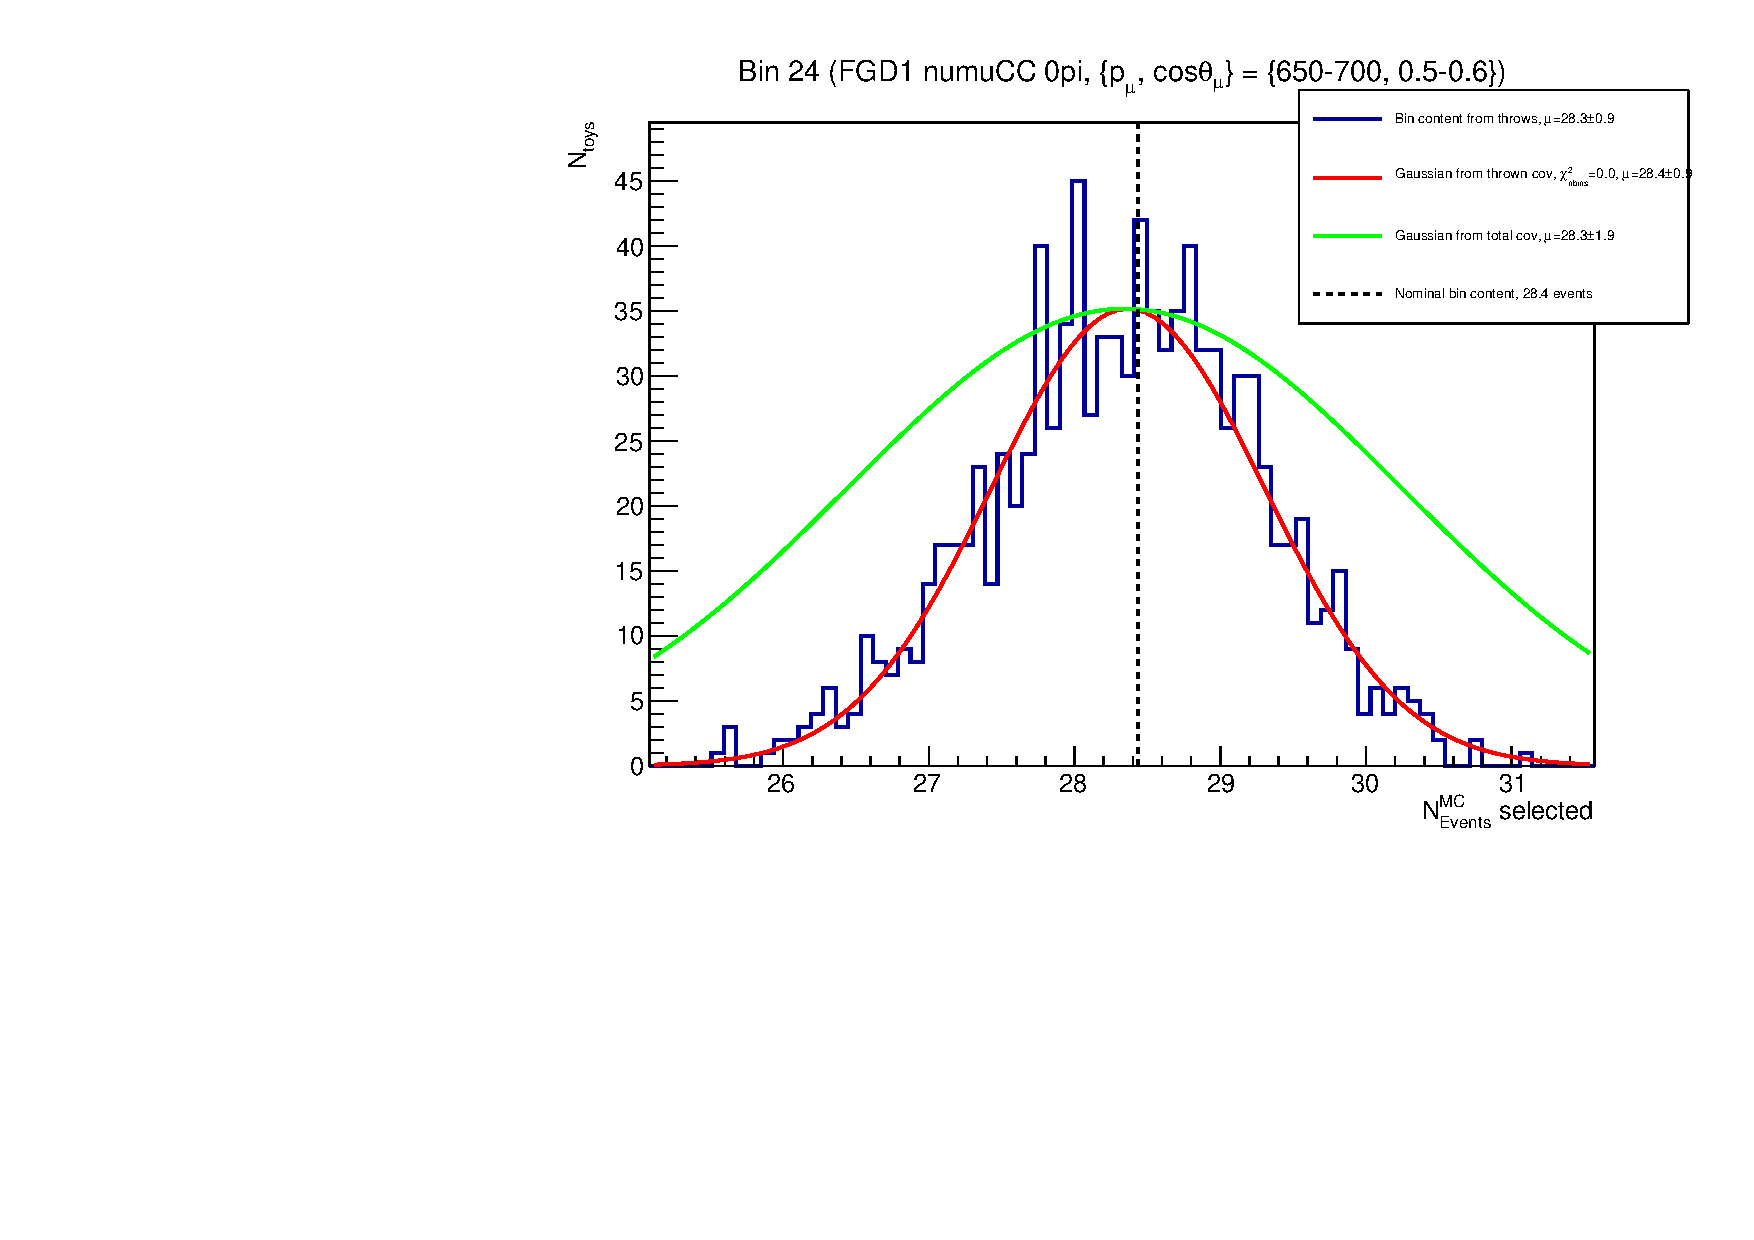
\includegraphics[width=\textwidth,page=1, trim={0mm 0mm 0mm 0mm}, clip]{figures/det/fgd1_numu_0pi_good}
	\end{subfigure}
	\begin{subfigure}[t]{0.32\textwidth}
		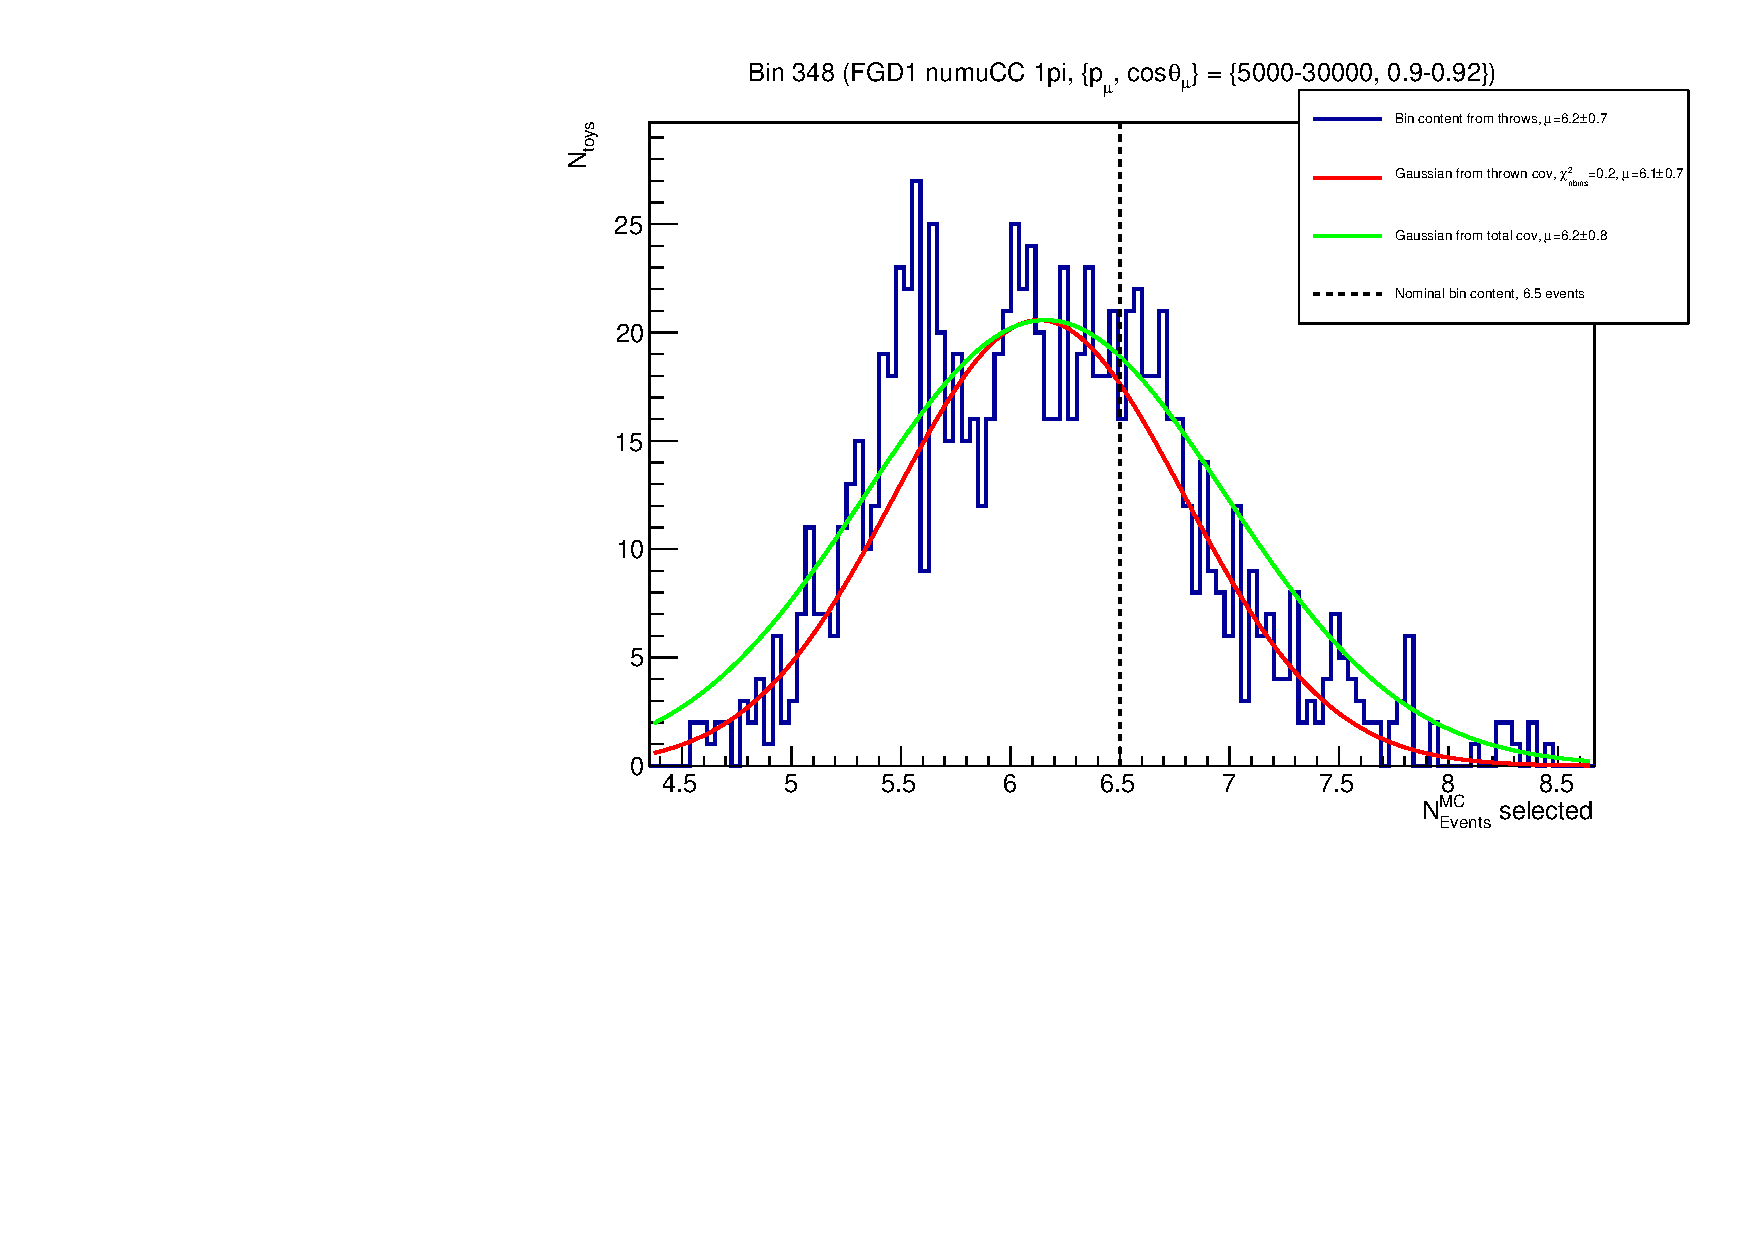
\includegraphics[width=\textwidth,page=1, trim={0mm 0mm 0mm 0mm}, clip]{figures/det/fgd1_numu_1pi_good}
	\end{subfigure}
	\begin{subfigure}[t]{0.32\textwidth}
		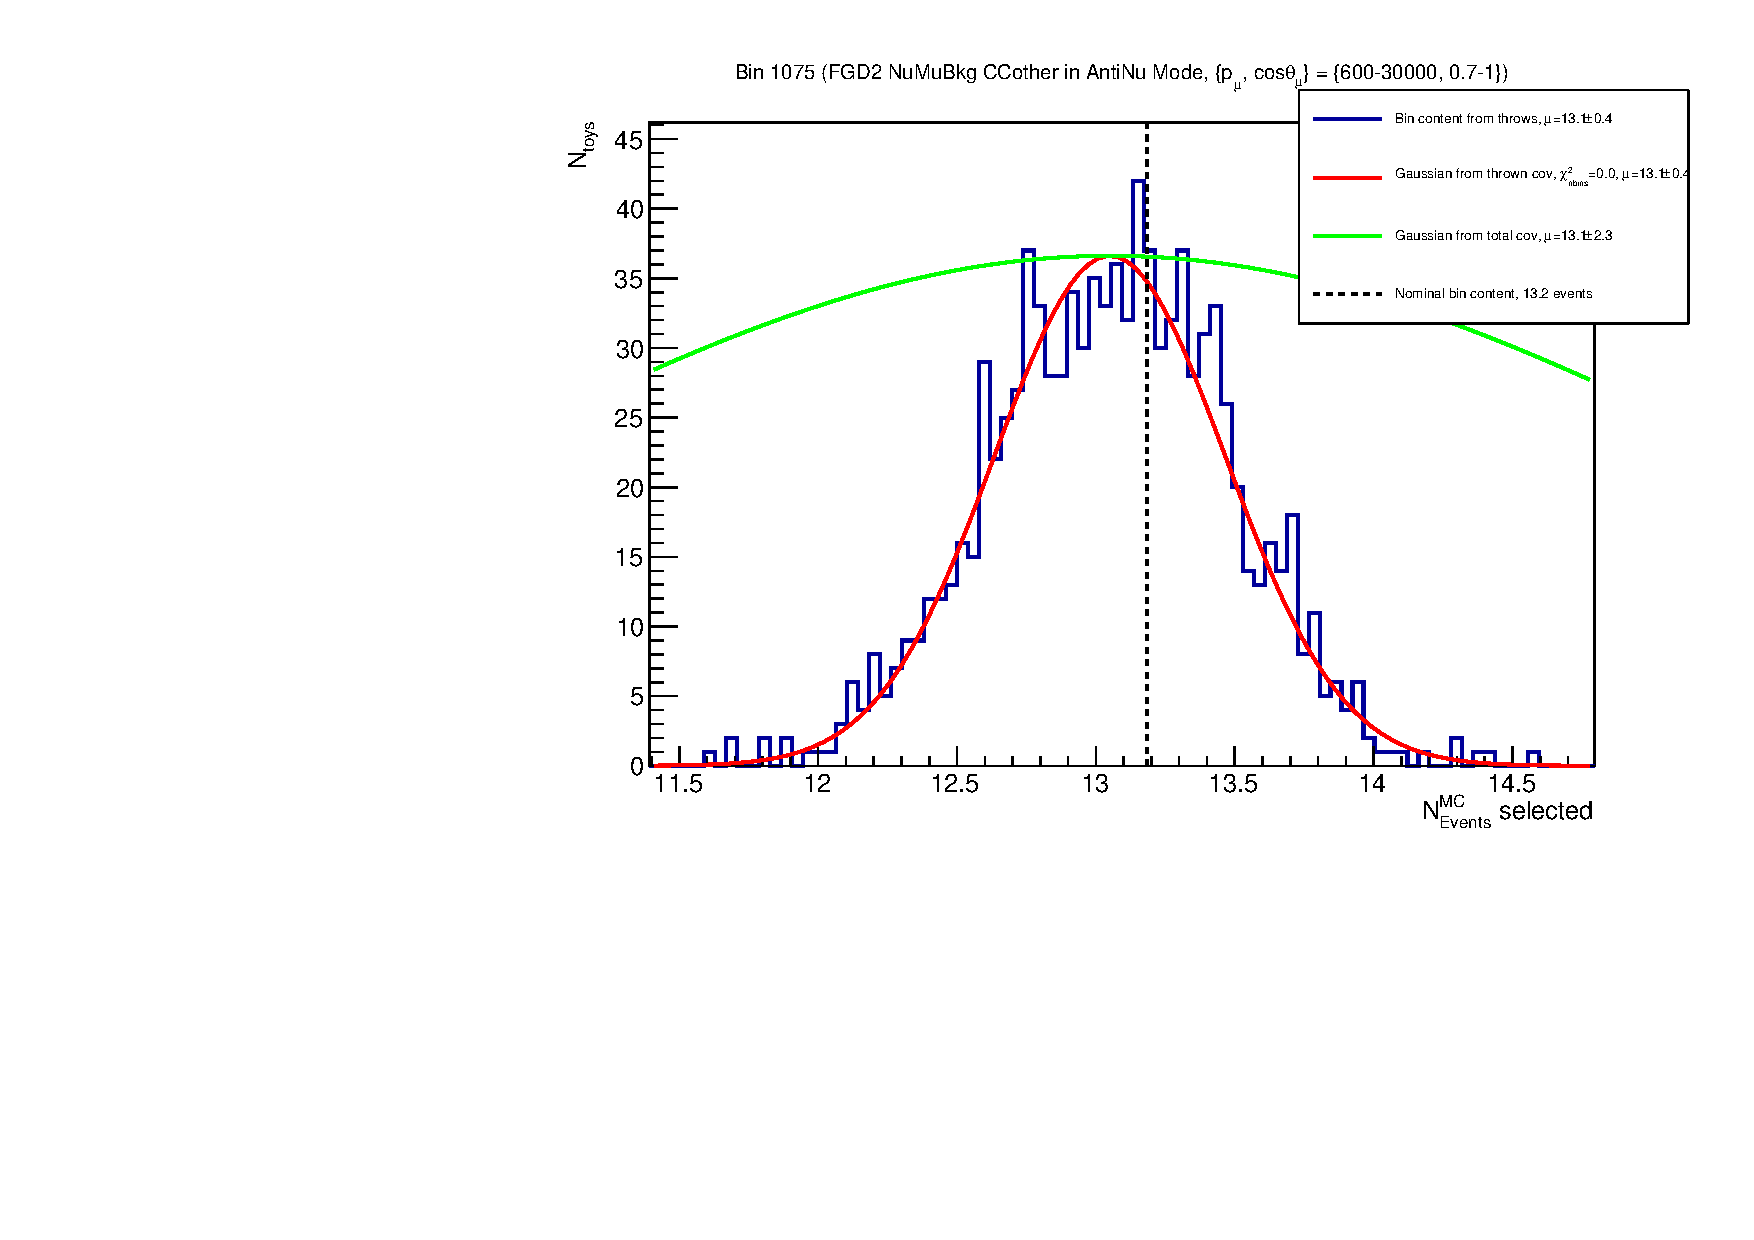
\includegraphics[width=\textwidth,page=1, trim={0mm 0mm 0mm 0mm}, clip]{figures/det/fgd2_numubkg_ccoth_good}
	\end{subfigure}
	\caption{Bin-by-bin event distributions with fitted Gaussians for the reduced ND280 systematic parameterisation}
	\label{fig:det_binbybin}
\end{figure}

The new ND280 covariance matrix is shown in \autoref{fig:nd280_cov_2018} and \autoref{fig:nd280_corr_2018}. Note: they are not directly comparable to the 2017 matrices in \autoref{fig:nd280_cov} and \autoref{fig:nd280_corr} because the dominant parameter switched from \pmu to \cosmu so parameters now run $\{\cos\theta_\mu^1,p_\mu^1\}, \{\cos\theta_\mu^1,p_\mu^2\},...\{\cos\theta_\mu^1,p_\mu^N\}$ instead of $\{\cos\theta_\mu^1,p_\mu^1\}, \{\cos\theta_\mu^2,p_\mu^1\},...\{\cos\theta_\mu^N,p_\mu^1\}$. However we note many similarities with 2017: the largest systematics are $\sim50\%$, notably in the high-momentum bins. FGD1 and FGD2 are correlated as expected, and the selections in each FGD is correlated more.
\begin{figure}[h]
	\includegraphics[width=0.7\textwidth,page=1, trim={0mm 0mm 0mm 0mm}, clip]{figures/det/2018_detmatrix}
	\caption{$\sqrt{\text{Covariance}}$ for the reduced ND280 parameterisation}
	\label{fig:nd280_cov_2018}
\end{figure}

\begin{figure}[h]
	\includegraphics[width=0.7\textwidth,page=4, trim={0mm 0mm 0mm 0mm}, clip]{figures/det/2018_detmatrix}
	\caption{Correlation for the reduced ND280 parameterisation}
	\label{fig:nd280_corr_2018}
\end{figure}

\subsection{The Neutrino-Matter Interaction}
The interaction systematics are similar to \autoref{subsec:syst_xsec} with two changes: a new FSI tune was developed, and an uncertainty on radiative corrections was applied.

\paragraph{Pion Final State Interactions}
The new FSI tune\cite{thesis_elder} did not change the underlying model, but applied a more robust fitting method, extending the scattering data to heavier targets such as oxygen, aluminium, iron and lead, including fresh data from the dedicated DUET experiment\cite{duet}. It was also decided to remove the high energy charge exchange pion final state parameter due to poor constraints from external data. The new constraints are shown in \autoref{tab:pion_fsi_2018}, and is a reduction for the quasi-elastic and charge exchange parameters, but is otherwise an inflation. The inelastic and quasi-elastic high energy probabilities double in uncertainty. The absorption and charge exchange central values move by $\sim1\sigma$ from the old recommendation. However, the correlations are now fully evaluated and the expectation is to reduce the systematics by $\sim50\%$.
\begin{table}[h]
	\begin{tabular}{l | c c}
		\hline
		\hline
		Parameter & 2017 value & Best-fit $\pm1\sigma$ \\
		\hline
		FEFQE & $1.0\pm0.41$ & $1.069\pm0.313$ \\
		FEFABS & $1.1\pm0.41$ & $1.404\pm0.432$ \\
		FEFCX & $1.0\pm0.57$ & $0.697\pm0.305$ \\
		FEFINEL & $1.0\pm0.50$ & $1.002\pm1.101$ \\
		FEFQEH & $1.8\pm0.34$ & $1.824\pm0.859$ \\
		\hline
		\hline
	\end{tabular}
\caption{New pion final state interaction central values and uncertainties introduced for 2018 analyses}
\label{tab:pion_fsi_2018}
\end{table}

\paragraph{Coulomb Corrections}
As the anti-neutrino statistics increased, a systematic was included to account for the Coulomb effect of a lepton leaving the interaction nucleon and nucleus. $\mu^+/e^+$ receive a repulsive force and $\mu^-/e^-$ an attractive force, and is simply modelled by shifting the true lepton momentum by a fixed amount, dependent on the target nucleus\cite{coulomb1, coulomb2}. The shifts are shown in \autoref{tab:coulomb_shifts}.
\begin{table}[h]
	\begin{tabular}{l | c c}
		$V_C$ (MeV) & $\mu^-$ & $\mu^+$ \\
		\hline
		$^{12}C$ & $-3.6$ & $+2.6$ \\
		$^{16}O$ & $-4.3$ & $+3.3$ \\
	\end{tabular}
		\caption{Lepton momentum shifts as a result of Coulomb corrections}
		\label{tab:coulomb_shifts}
\end{table}

Since the relative effect of the Coulomb shift is smaller at higher momentum, a correlated 3\% total (2\% on $\nu$, 1\% on $\bar{\nu}$ negatively correlated with each other) uncertainty on CC inclusive $\nu$ and $\bar{\nu}$ with $0.4 < E_\nu < 0.6 \text{ GeV}$ is applied.

\paragraph{Covariance Matrix}
The new covariance and correlation matrices for the interaction systematics are presented in \autoref{fig:xsec_cov_2018} and \autoref{fig:xsec_corr_2018}. As previously noted, the pion FSI parameters (upper right corner) are now fully correlated which gives rise to smaller overall pion FSI systematics. The new CC normalisation from uncertainties in the Coulomb correction is shown in the middle of the matrix.
\begin{figure}[h]
	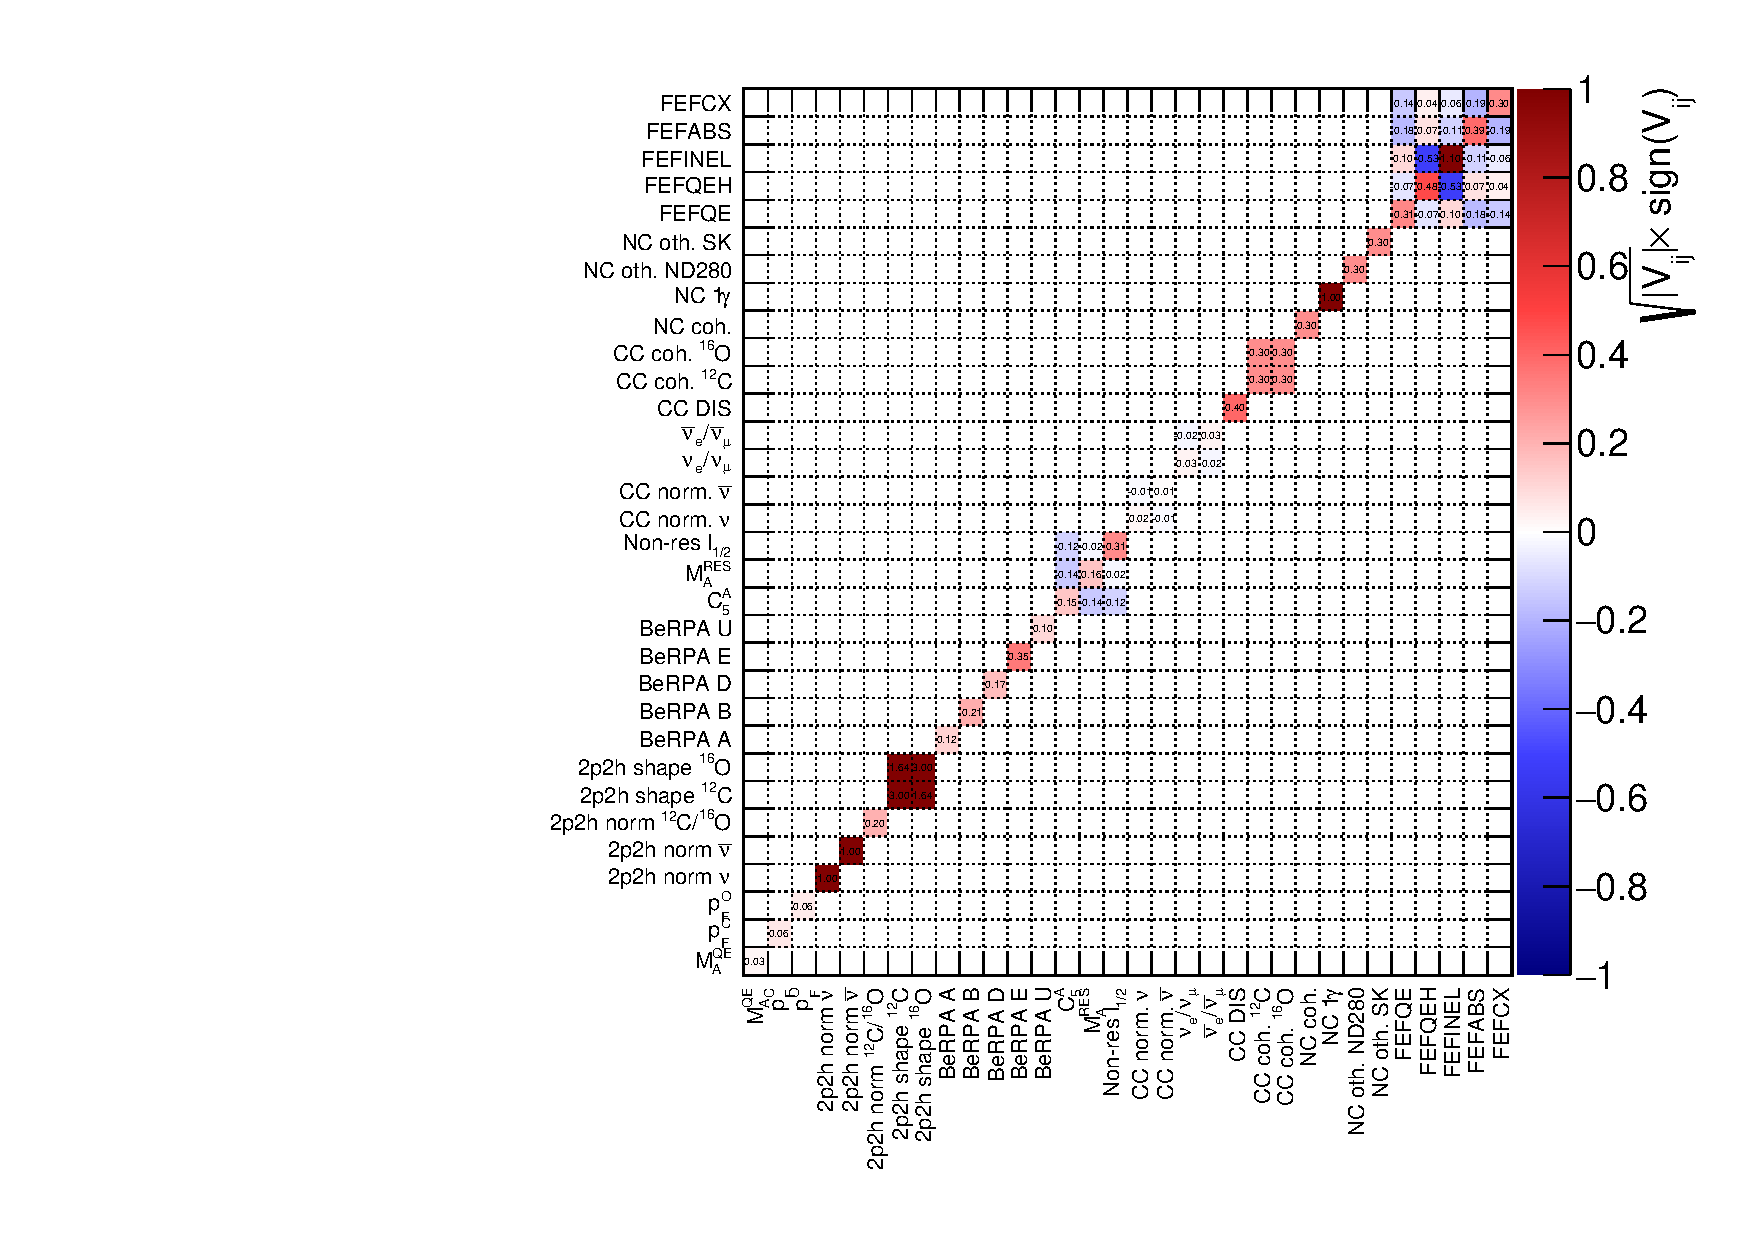
\includegraphics[width=0.7\textwidth,page=1, trim={0mm 0mm 0mm 0mm}, clip]{figures/niwg/xsec_covariance_2018a_NOMINAL_v11_xseccov}
	\caption{$\sqrt{\text{Covariance}}$ for the interaction parameters in 2018}
	\label{fig:xsec_cov_2018}
\end{figure}

\begin{figure}[h]
	\includegraphics[width=0.7\textwidth,page=2, trim={0mm 0mm 0mm 0mm}, clip]{figures/niwg/xsec_covariance_2018a_NOMINAL_v11_xseccov}
	\caption{Correlation for the interaction parameters in 2018}
	\label{fig:xsec_corr_2018}
\end{figure}

\clearpage
\section{Nominal Model Prediction}
Using the nominal model, applying the multiplicative nominal weights, the event rates in \autoref{tab:detailed_eventrate_2018} are obtained.

As expected from the large increase in POT detailed in \autoref{tab:pot_2018}, run 7 and 8 almost doubles the data for the FHC and RHC selections. There are now 67,000 FHC \numu, 13,000 RHC \numubar, and 5,000 RHC \numu CC0$\pi$ events, totalling at 82,000. The FGD1 and FGD2 equivalent selections are consistent, and we generally note CC0$\pi$ selections underestimated by 0-6\%, CC1$\pi$ overestimated by the same amount, and CCOther underestimated by 9-26\% for all FGDs and beam running modes. Averaging over all the selections the nominal model underestimates the data by 6\%.

% Full matrix
%\begin{table}[h]
%	\centering
%	\begin{tabular}{ l c c c }
%		\hline
 %       \hline
%		Sample & Data & Nominal MC & Data/MC \\
%		\hline
%		FGD1 0$\pi$       & 33553 & 31530.5  & 1.06 \\
%		FGD1 1$\pi$       & 7757  & 7997.96  & 0.97 \\
%		FGD1 Other        & 8068  & 6793.11  & 1.18 \\
%		\hline
%		FGD2 0$\pi$       & 33462 & 31736.7 & 1.05\\
%		FGD2 1$\pi$       & 6133  & 6419.23 & 0.96 \\
%		FGD2 Other        & 7664  & 6563.14 & 1.17 \\
%		\hline
%		FGD1 \numubar 0$\pi$       & 6368 & 6371.09  & 1.00 \\
%		FGD1 \numubar 1$\pi$       & 535  & 533.187  & 1.00 \\
%		FGD1 \numubar Other        & 1032 & 1023.2  & 1.01 \\
%		\hline
%		FGD2 \numubar 0$\pi$       & 6451 & 6284.65  & 1.03  \\
%		FGD2 \numubar 1$\pi$       & 465  & 483.469  & 0.96 \\
%		FGD2 \numubar Other        & 1032 & 944.175 & 1.09 \\
%		\hline
%		FGD1 \numu RHC 0$\pi$       & 2707 & 2497.71 & 1.08 \\
%		FGD1 \numu RHC 1$\pi$       & 847  & 860.675 & 0.98 \\
%		FGD1 \numu RHC Other        & 1015 & 797.499 & 1.27 \\
%		\hline
%		FGD2 \numu RHC 0$\pi$       & 2648 & 2553.51 & 1.04 \\
%		FGD2 \numu RHC 1$\pi$       & 693  & 679.99  & 1.02 \\
%		FGD2 \numu RHC Other        & 932  & 792.166 & 1.18 \\
 %               \hline
%		Total & 121432 & 114862 & 1.06 \\
%		Total x2017 & 1.87 & 1.80 & \\
%		\hline
%		\hline
%	\end{tabular}
 %       \caption{Based on full matrix hAdNOT heppc205 8 Apr and DsHVqI on heppc105}
%	\label{tab:detailed_eventrate_2018}
%\end{table}

% Reduced matrix,  fLrRiy on 205
\begin{table}[h]
  \begin{tabular}{l c c c }
  	\hline
  	\hline
  	Sample & Data & Nominal MC & Data/MC \\
  	\hline
    FGD1 0$\pi$          & 33553     & 31529.3 & 1.06  \\
    FGD1 1$\pi$          & 7757      & 7998.1  & 0.97 \\
    FGD1 other           & 8068      & 6793.68 & 1.18 \\
    \hline
    FGD2 0$\pi$          & 33462     & 31734   & 1.05 \\
    FGD2 1$\pi$          & 6133      & 6419.04 & 0.96 \\
    FGD2 other           & 7664      & 6562.75 & 1.17 \\
    \hline
    FGD1 \numubar 0$\pi$       & 6368      & 6371.34 & 1.00 \\
    FGD1 \numubar 1$\pi$       & 535       & 533.253 & 1.00 \\
    FGD1 \numubar other        & 1102      & 1023.36 & 1.08 \\
    \hline
    FGD2 \numubar 0$\pi$       & 6451      & 6283.35 & 1.03\\
    FGD2 \numubar 1$\pi$       & 465       & 483.508 & 0.96 \\
    FGD2 \numubar other        & 1032      & 943.956 & 1.09 \\
    \hline
    FGD1 \numu RHC 0$\pi$ 	   & 2707      & 2485.51 & 1.09 \\
    FGD1 \numu RHC 1$\pi$		& 847      & 855.911 & 0.99 \\
    FGD1 \numu RHC other 	   & 1015      & 804.647 & 1.26\\
    \hline
    FGD2 \numu RHC 0$\pi$ 		& 2648      & 2553.51 & 1.04 \\
    FGD2 \numu RHC 1$\pi$ 		& 693       & 679.99  & 1.02 \\
    FGD2 \numu RHC other 		& 932       & 792.166 & 1.18 \\
    \hline
    Total                       & 121432  	& 114847 & 1.06 \\
    Total x2017					& 1.87 		& 1.80 \\
    \hline
    \hline
  \end{tabular}
  \caption{Observed and predicted event rates for the different ND280 selections for the 2018 analysis}
  \label{tab:detailed_eventrate_2018}
\end{table}

\autoref{fig:nominal2D_FGD1numu_2018} shows the data and nominal model prediction for the FGD1 FHC selections. We see in the restricted plotting region (excluding highest momentum and most backward bins, normalising to bin width), the data is consistently higher than the prediction. The CC0$\pi$ selection looks overestimated at higher momentum between \cosmu=0.8-0.95. We also see some clear underestimates along lines of constant $Q^2$, between 0.07 and 0.15 $\text{GeV}^2$. For the CC1$\pi$ selection we see a similar overestimate at high \pmu and \cosmu=0.8-0.95. For the CCOther selection we see a clear underestimate in almost all bins below $Q^2=0.2\text{ GeV}^2$. In general, the distributions are compatible and similar to the 2017 equivalents in \autoref{fig:nominal2D_FGD1numu}.
\begin{figure}[h]
	\begin{subfigure}[t]{0.32\textwidth}
		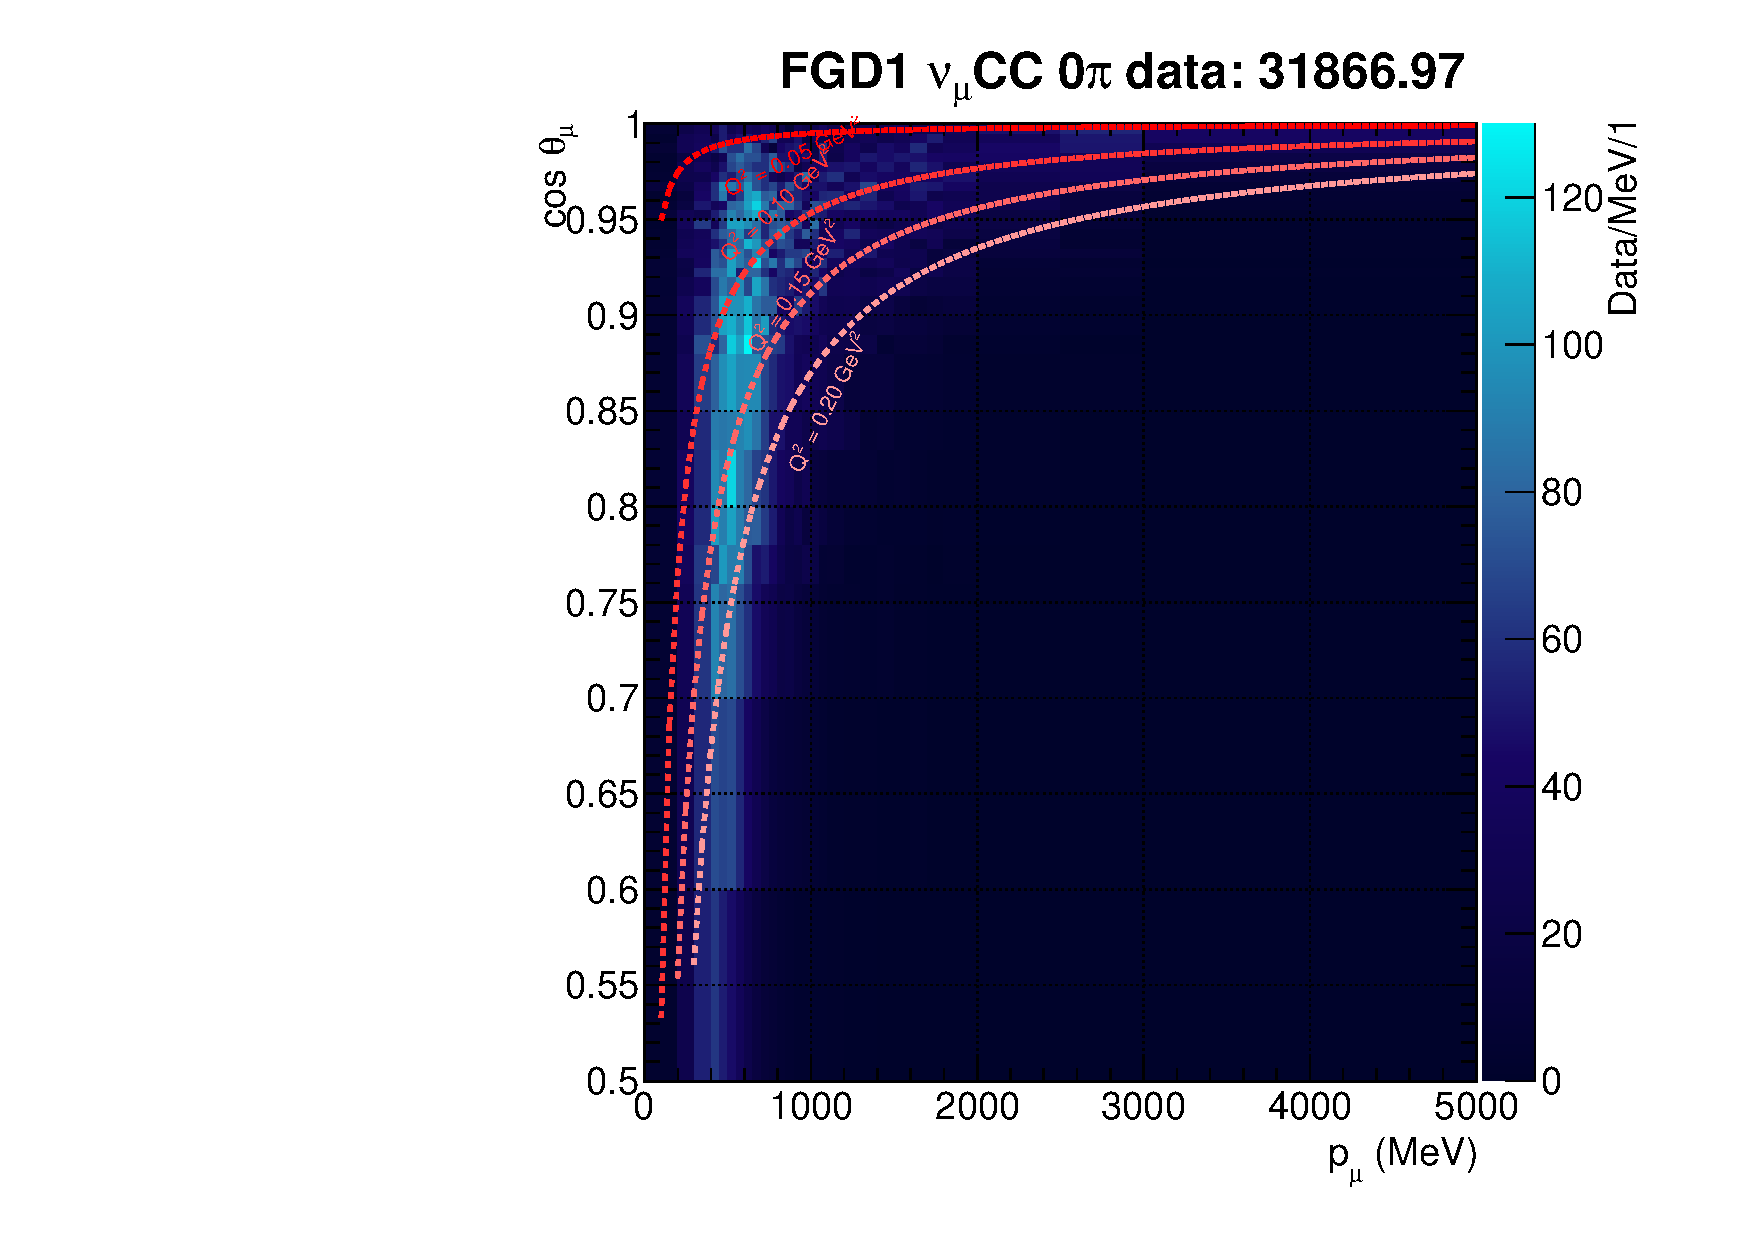
\includegraphics[width=\textwidth,page=1]{{figures/mach3/2018/Selection/2018_RedNDmatrix_rebin_verbose_may_noweights_ND280_nom}}
	\end{subfigure}
	\begin{subfigure}[t]{0.32\textwidth}
		\includegraphics[width=\textwidth,page=2]{{figures/mach3/2018/Selection/2018_RedNDmatrix_rebin_verbose_may_noweights_ND280_nom}}
	\end{subfigure}
	\begin{subfigure}[t]{0.32\textwidth}
		\includegraphics[width=\textwidth,page=3]{{figures/mach3/2018/Selection/2018_RedNDmatrix_rebin_verbose_may_noweights_ND280_nom}}
	\end{subfigure}
	
	\begin{subfigure}[t]{0.32\textwidth}
		\includegraphics[width=\textwidth,page=4]{{figures/mach3/2018/Selection/2018_RedNDmatrix_rebin_verbose_may_noweights_ND280_nom}}
	\end{subfigure}
	\begin{subfigure}[t]{0.32\textwidth}
		\includegraphics[width=\textwidth,page=5]{{figures/mach3/2018/Selection/2018_RedNDmatrix_rebin_verbose_may_noweights_ND280_nom}}
	\end{subfigure}
	\begin{subfigure}[t]{0.32\textwidth}
		\includegraphics[width=\textwidth,page=6]{{figures/mach3/2018/Selection/2018_RedNDmatrix_rebin_verbose_may_noweights_ND280_nom}}
	\end{subfigure}
	
	\begin{subfigure}[t]{0.32\textwidth}
		\includegraphics[width=\textwidth,page=7]{{figures/mach3/2018/Selection/2018_RedNDmatrix_rebin_verbose_may_noweights_ND280_nom}}
	\end{subfigure}
	\begin{subfigure}[t]{0.32\textwidth}
		\includegraphics[width=\textwidth,page=8]{{figures/mach3/2018/Selection/2018_RedNDmatrix_rebin_verbose_may_noweights_ND280_nom}}
	\end{subfigure}
	\begin{subfigure}[t]{0.32\textwidth}
		\includegraphics[width=\textwidth,page=9]{{figures/mach3/2018/Selection/2018_RedNDmatrix_rebin_verbose_may_noweights_ND280_nom}}
	\end{subfigure}
	
	\caption{Data and nominal MC distributions and the Data/MC ratio for FGD1 FHC selections. Lines of constant $Q^2_\text{reco}$ are shown. Bin content is normalised to bin width.}
	\label{fig:nominal2D_FGD1numu_2018}
\end{figure}

\autoref{fig:nominal2D_FGD2numu_2018} shows the nominal FHC \numu distributions for FGD2, with very similar behaviour to the FGD1 distributions.
\begin{figure}[h]
	\begin{subfigure}[t]{0.32\textwidth}
		\includegraphics[width=\textwidth,page=10]{{figures/mach3/2018/Selection/2018_RedNDmatrix_rebin_verbose_may_noweights_ND280_nom}}
	\end{subfigure}
	\begin{subfigure}[t]{0.32\textwidth}
		\includegraphics[width=\textwidth,page=11]{{figures/mach3/2018/Selection/2018_RedNDmatrix_rebin_verbose_may_noweights_ND280_nom}}
	\end{subfigure}
	\begin{subfigure}[t]{0.32\textwidth}
		\includegraphics[width=\textwidth,page=12]{{figures/mach3/2018/Selection/2018_RedNDmatrix_rebin_verbose_may_noweights_ND280_nom}}
	\end{subfigure}
	
	\begin{subfigure}[t]{0.32\textwidth}
		\includegraphics[width=\textwidth,page=13]{{figures/mach3/2018/Selection/2018_RedNDmatrix_rebin_verbose_may_noweights_ND280_nom}}
	\end{subfigure}
	\begin{subfigure}[t]{0.32\textwidth}
		\includegraphics[width=\textwidth,page=14]{{figures/mach3/2018/Selection/2018_RedNDmatrix_rebin_verbose_may_noweights_ND280_nom}}
	\end{subfigure}
	\begin{subfigure}[t]{0.32\textwidth}
		\includegraphics[width=\textwidth,page=15]{{figures/mach3/2018/Selection/2018_RedNDmatrix_rebin_verbose_may_noweights_ND280_nom}}
	\end{subfigure}
	
	\begin{subfigure}[t]{0.32\textwidth}
		\includegraphics[width=\textwidth,page=16]{{figures/mach3/2018/Selection/2018_RedNDmatrix_rebin_verbose_may_noweights_ND280_nom}}
	\end{subfigure}
	\begin{subfigure}[t]{0.32\textwidth}
		\includegraphics[width=\textwidth,page=17]{{figures/mach3/2018/Selection/2018_RedNDmatrix_rebin_verbose_may_noweights_ND280_nom}}
	\end{subfigure}
	\begin{subfigure}[t]{0.32\textwidth}
		\includegraphics[width=\textwidth,page=18]{{figures/mach3/2018/Selection/2018_RedNDmatrix_rebin_verbose_may_noweights_ND280_nom}}
	\end{subfigure}
	
	\caption{Data and nominal MC distributions and the Data/MC ratio for FGD2 FHC selections. Lines of constant $Q^2_\text{reco}$ are shown. Bin content is normalised to bin width.}
	\label{fig:nominal2D_FGD2numu_2018}
\end{figure}

\autoref{fig:nominal2D_FGD1numubar_2018} shows the first light for the new RHC CC0$\pi$, CC1$\pi$ and CCNTrack selections. The CC0$\pi$ selection is slightly over-estimated, but the nominal prediction looks more compatible with data than the FHC \numu distributions. The Data/MC ratio also doesn't appear to contain the same deficiency in $Q^2$. The CC1$\pi$ distribution is consistently underestimated in the most forward bin, and hints at an overestimation at low $Q^2$. The CCOther distribution looks similar to the FHC equivalents in that it is almost consistently underestimated.
\begin{figure}
	\begin{subfigure}[t]{0.32\textwidth}
		\includegraphics[width=\textwidth,page=19]{{figures/mach3/2018/Selection/2018_RedNDmatrix_rebin_verbose_may_noweights_ND280_nom}}
	\end{subfigure}
	\begin{subfigure}[t]{0.32\textwidth}
		\includegraphics[width=\textwidth,page=20]{{figures/mach3/2018/Selection/2018_RedNDmatrix_rebin_verbose_may_noweights_ND280_nom}}
	\end{subfigure}
	\begin{subfigure}[t]{0.32\textwidth}
		\includegraphics[width=\textwidth,page=21]{{figures/mach3/2018/Selection/2018_RedNDmatrix_rebin_verbose_may_noweights_ND280_nom}}
	\end{subfigure}
	
	\begin{subfigure}[t]{0.32\textwidth}
		\includegraphics[width=\textwidth,page=22]{{figures/mach3/2018/Selection/2018_RedNDmatrix_rebin_verbose_may_noweights_ND280_nom}}
	\end{subfigure}
	\begin{subfigure}[t]{0.32\textwidth}
		\includegraphics[width=\textwidth,page=23]{{figures/mach3/2018/Selection/2018_RedNDmatrix_rebin_verbose_may_noweights_ND280_nom}}
	\end{subfigure}
	\begin{subfigure}[t]{0.32\textwidth}
		\includegraphics[width=\textwidth,page=24]{{figures/mach3/2018/Selection/2018_RedNDmatrix_rebin_verbose_may_noweights_ND280_nom}}
	\end{subfigure}
	
	\begin{subfigure}[t]{0.32\textwidth}
		\includegraphics[width=\textwidth,page=25]{{figures/mach3/2018/Selection/2018_RedNDmatrix_rebin_verbose_may_noweights_ND280_nom}}
	\end{subfigure}
	\begin{subfigure}[t]{0.32\textwidth}
		\includegraphics[width=\textwidth,page=26]{{figures/mach3/2018/Selection/2018_RedNDmatrix_rebin_verbose_may_noweights_ND280_nom}}
	\end{subfigure}
	\begin{subfigure}[t]{0.32\textwidth}
		\includegraphics[width=\textwidth,page=27]{{figures/mach3/2018/Selection/2018_RedNDmatrix_rebin_verbose_may_noweights_ND280_nom}}
	\end{subfigure}
	\caption{Data and nominal MC distributions and the Data/MC ratio for FGD1 \numubar selections. Lines of constant $Q^2_\text{reco}$ are shown. Bin content is normalised to bin width.}
	\label{fig:nominal2D_FGD1numubar_2018}
\end{figure}

\autoref{fig:nominal2D_FGD2numubar_2018} shows the new RHC selections for FGD2. The CC0$\pi$ distribution is underestimated, in contrast to FGD1, and looks more similar to the FHC selections with patters of underestimation looking roughly constant in $Q^2$. The CC1$\pi$ distribution appears to underestimate in $Q^2$ rather than overestimate as was the case for FGD1. The CCOther distribution however largely looks compatible with the FGD1 case and is underestimated in general.
\begin{figure}
	\begin{subfigure}[t]{0.32\textwidth}
		\includegraphics[width=\textwidth,page=28]{{figures/mach3/2018/Selection/2018_RedNDmatrix_rebin_verbose_may_noweights_ND280_nom}}
	\end{subfigure}
	\begin{subfigure}[t]{0.32\textwidth}
		\includegraphics[width=\textwidth,page=29]{{figures/mach3/2018/Selection/2018_RedNDmatrix_rebin_verbose_may_noweights_ND280_nom}}
	\end{subfigure}
	\begin{subfigure}[t]{0.32\textwidth}
		\includegraphics[width=\textwidth,page=30]{{figures/mach3/2018/Selection/2018_RedNDmatrix_rebin_verbose_may_noweights_ND280_nom}}
	\end{subfigure}

	\begin{subfigure}[t]{0.32\textwidth}
		\includegraphics[width=\textwidth,page=31]{{figures/mach3/2018/Selection/2018_RedNDmatrix_rebin_verbose_may_noweights_ND280_nom}}
	\end{subfigure}
	\begin{subfigure}[t]{0.32\textwidth}
		\includegraphics[width=\textwidth,page=32]{{figures/mach3/2018/Selection/2018_RedNDmatrix_rebin_verbose_may_noweights_ND280_nom}}
	\end{subfigure}
	\begin{subfigure}[t]{0.32\textwidth}
		\includegraphics[width=\textwidth,page=33]{{figures/mach3/2018/Selection/2018_RedNDmatrix_rebin_verbose_may_noweights_ND280_nom}}
	\end{subfigure}
	
	\begin{subfigure}[t]{0.32\textwidth}
		\includegraphics[width=\textwidth,page=34]{{figures/mach3/2018/Selection/2018_RedNDmatrix_rebin_verbose_may_noweights_ND280_nom}}
	\end{subfigure}
	\begin{subfigure}[t]{0.32\textwidth}
		\includegraphics[width=\textwidth,page=35]{{figures/mach3/2018/Selection/2018_RedNDmatrix_rebin_verbose_may_noweights_ND280_nom}}
	\end{subfigure}
	\begin{subfigure}[t]{0.32\textwidth}
		\includegraphics[width=\textwidth,page=36]{{figures/mach3/2018/Selection/2018_RedNDmatrix_rebin_verbose_may_noweights_ND280_nom}}
	\end{subfigure}	
\caption{Data and nominal MC distributions and the Data/MC ratio for FGD2 \numubar selections. Lines of constant $Q^2_\text{reco}$ are shown. Bin content is normalised to bin width.}
\label{fig:nominal2D_FGD2numubar_2018}
\end{figure}

\autoref{fig:nominal2D_FGD1numurhc_2018} shows the new RHC \numu selections for FGD1. As expected, they are concentrated at higher $p_\mu$, owing to the neutrino parents producing neutrinos of higher $E_\nu$. The distributions are consistently underestimated, although the shapes are fairly well reproduced. The CC0$\pi$ distribution again looks underestimated in constant $Q^2$, similar to the FHC \numu and RHC \numubar selections. The CC1$\pi$ selection is also similar to the RHC \numubar equivalent and is underestimated at high \cosmu and high \pmu. The CCOther selection agrees well with the previous CCOther selections, being even more underestimated than for the others.
\begin{figure}[h]
	\begin{subfigure}[t]{0.32\textwidth}
		\includegraphics[width=\textwidth,page=37]{{figures/mach3/2018/Selection/2018_RedNDmatrix_rebin_verbose_may_noweights_ND280_nom}}
	\end{subfigure}
	\begin{subfigure}[t]{0.32\textwidth}
		\includegraphics[width=\textwidth,page=38]{{figures/mach3/2018/Selection/2018_RedNDmatrix_rebin_verbose_may_noweights_ND280_nom}}
	\end{subfigure}
	\begin{subfigure}[t]{0.32\textwidth}
		\includegraphics[width=\textwidth,page=39]{{figures/mach3/2018/Selection/2018_RedNDmatrix_rebin_verbose_may_noweights_ND280_nom}}
	\end{subfigure}

	\begin{subfigure}[t]{0.32\textwidth}
		\includegraphics[width=\textwidth,page=40]{{figures/mach3/2018/Selection/2018_RedNDmatrix_rebin_verbose_may_noweights_ND280_nom}}
	\end{subfigure}
	\begin{subfigure}[t]{0.32\textwidth}
		\includegraphics[width=\textwidth,page=41]{{figures/mach3/2018/Selection/2018_RedNDmatrix_rebin_verbose_may_noweights_ND280_nom}}
	\end{subfigure}
	\begin{subfigure}[t]{0.32\textwidth}
		\includegraphics[width=\textwidth,page=42]{{figures/mach3/2018/Selection/2018_RedNDmatrix_rebin_verbose_may_noweights_ND280_nom}}
	\end{subfigure}

	\begin{subfigure}[t]{0.32\textwidth}
		\includegraphics[width=\textwidth,page=43]{{figures/mach3/2018/Selection/2018_RedNDmatrix_rebin_verbose_may_noweights_ND280_nom}}
	\end{subfigure}
	\begin{subfigure}[t]{0.32\textwidth}
		\includegraphics[width=\textwidth,page=44]{{figures/mach3/2018/Selection/2018_RedNDmatrix_rebin_verbose_may_noweights_ND280_nom}}
	\end{subfigure}
	\begin{subfigure}[t]{0.32\textwidth}
		\includegraphics[width=\textwidth,page=45]{{figures/mach3/2018/Selection/2018_RedNDmatrix_rebin_verbose_may_noweights_ND280_nom}}
	\end{subfigure}
\caption{Data and nominal MC distributions and the Data/MC ratio for FGD1 \numu RHC selections. Lines of constant $Q^2_\text{reco}$ are shown. Bin content is normalised to bin width.}
\label{fig:nominal2D_FGD1numurhc_2018}
\end{figure}

The FGD2 \numu RHC distributions in \autoref{fig:nominal2D_FGD2numurhc_2018} are similarly underestimated throughout. For CC0$\pi$ there is consistent underestimation at high \pmu and \cosmu, which agrees with the FGD1 distribution. The data appears shifted towards higher momentum to the prediction, and have a larger spread. The CC1$\pi$ selection is similarly patchy and is difficult to draw conclusions from. CCOther is consistent with FGD1, being mostly underestimated, although overestimated at low momentum.
\begin{figure}[h]
	\begin{subfigure}[t]{0.32\textwidth}
		\includegraphics[width=\textwidth,page=46]{{figures/mach3/2018/Selection/2018_RedNDmatrix_rebin_verbose_may_noweights_ND280_nom}}
	\end{subfigure}
	\begin{subfigure}[t]{0.32\textwidth}
		\includegraphics[width=\textwidth,page=47]{{figures/mach3/2018/Selection/2018_RedNDmatrix_rebin_verbose_may_noweights_ND280_nom}}
	\end{subfigure}
	\begin{subfigure}[t]{0.32\textwidth}
		\includegraphics[width=\textwidth,page=48]{{figures/mach3/2018/Selection/2018_RedNDmatrix_rebin_verbose_may_noweights_ND280_nom}}
	\end{subfigure}
	
	\begin{subfigure}[t]{0.32\textwidth}
		\includegraphics[width=\textwidth,page=49]{{figures/mach3/2018/Selection/2018_RedNDmatrix_rebin_verbose_may_noweights_ND280_nom}}
	\end{subfigure}
	\begin{subfigure}[t]{0.32\textwidth}
		\includegraphics[width=\textwidth,page=50]{{figures/mach3/2018/Selection/2018_RedNDmatrix_rebin_verbose_may_noweights_ND280_nom}}
	\end{subfigure}
	\begin{subfigure}[t]{0.32\textwidth}
		\includegraphics[width=\textwidth,page=51]{{figures/mach3/2018/Selection/2018_RedNDmatrix_rebin_verbose_may_noweights_ND280_nom}}
	\end{subfigure}
	
	\begin{subfigure}[t]{0.32\textwidth}
		\includegraphics[width=\textwidth,page=52]{{figures/mach3/2018/Selection/2018_RedNDmatrix_rebin_verbose_may_noweights_ND280_nom}}
	\end{subfigure}
	\begin{subfigure}[t]{0.32\textwidth}
		\includegraphics[width=\textwidth,page=53]{{figures/mach3/2018/Selection/2018_RedNDmatrix_rebin_verbose_may_noweights_ND280_nom}}
	\end{subfigure}
	\begin{subfigure}[t]{0.32\textwidth}
		\includegraphics[width=\textwidth,page=54]{{figures/mach3/2018/Selection/2018_RedNDmatrix_rebin_verbose_may_noweights_ND280_nom}}
	\end{subfigure}
	\caption{Data and nominal MC distributions and the Data/MC ratio for FGD2 \numu RHC selections. Lines of constant $Q^2_\text{reco}$ are shown. Bin content is normalised to bin width.}
	\label{fig:nominal2D_FGD2numurhc_2018}
\end{figure}

Looking closer at the nominal distributions, we project onto \pmu and \cosmu separately and look at the mode contributions in the nominal model. The distributions for FGD1 FHC \numu selections are shown in \autoref{fig:nominal1D_pmu_fhc_2018}. For CC0$\pi$ we see the same behaviour as in 2017 (\autoref{fig:nominal1D_pmu}), with the low momentum on underestimated up until the event peak at 500 MeV, which after 1 GeV is mostly well modelled. The CC1$\pi$ distributions look marginally more consistent with data compared to 2017, but there is still a consistent overestimation in $0.5 < p_\mu < 1\text{ GeV}$, with a slight underestimation at the event peak. The CCOther distributions are again grossly underestimated throughout $p_\mu$ between 10 and 20\%. FGD2 looks particularly like a normalisation effect.
\begin{figure}[h]
	\begin{subfigure}[t]{0.20\textwidth}
		\includegraphics[width=\textwidth,page=55]{{figures/mach3/2018/Selection/2018_RedNDmatrix_rebin_verbose_may_noweights_ND280_nom}}
	\end{subfigure}

	\begin{subfigure}[t]{0.32\textwidth}
		\includegraphics[width=\textwidth,page=56]{{figures/mach3/2018/Selection/2018_RedNDmatrix_rebin_verbose_may_noweights_ND280_nom}}
	\end{subfigure}
	\begin{subfigure}[t]{0.32\textwidth}
		\includegraphics[width=\textwidth,page=58]{{figures/mach3/2018/Selection/2018_RedNDmatrix_rebin_verbose_may_noweights_ND280_nom}}
	\end{subfigure}
	\begin{subfigure}[t]{0.32\textwidth}
		\includegraphics[width=\textwidth,page=60]{{figures/mach3/2018/Selection/2018_RedNDmatrix_rebin_verbose_may_noweights_ND280_nom}}
	\end{subfigure}
	
	\begin{subfigure}[t]{0.32\textwidth}
		\includegraphics[width=\textwidth,page=62]{{figures/mach3/2018/Selection/2018_RedNDmatrix_rebin_verbose_may_noweights_ND280_nom}}
	\end{subfigure}
	\begin{subfigure}[t]{0.32\textwidth}
		\includegraphics[width=\textwidth,page=64]{{figures/mach3/2018/Selection/2018_RedNDmatrix_rebin_verbose_may_noweights_ND280_nom}}
	\end{subfigure}
	\begin{subfigure}[t]{0.32\textwidth}
		\includegraphics[width=\textwidth,page=66]{{figures/mach3/2018/Selection/2018_RedNDmatrix_rebin_verbose_may_noweights_ND280_nom}}
	\end{subfigure}

\caption{Data and nominal MC distributions for FHC \numu selections projected onto \pmu, showing contributions by interaction mode. Bin content is normalised to bin width.}
\label{fig:nominal1D_pmu_fhc_2018}
\end{figure}

The new RHC \numubar distributions' projections are shown in \autoref{fig:nominal1D_pmu_rhc_numubar_2018}, where the 0$\pi$ selection shows a similar pattern to the FHC \numu projections above and the 1Trk distributions from 2017. Namely, there is an underestimation at low $p_\mu$, which goes to an overestimation at $\sim0.5\text{ GeV}$, which returns to a satisfactory prediction above 1 GeV. FGD1 appears to see this more than FGD2, as was the case in 2017. For the 1$\pi$ selections, the prediction is mostly within 1$\sigma$ of the data (excluding systematic errors on the Monte Carlo). For the CCOther distributions there are hints of a consistent underestimation for both FGDs---particularly at lower momentum---but the majority of the prediction is still within statistical error of the data.
\begin{figure}[h]
	
	\begin{subfigure}[t]{0.32\textwidth}
		\includegraphics[width=\textwidth,page=68]{{figures/mach3/2018/Selection/2018_RedNDmatrix_rebin_verbose_may_noweights_ND280_nom}}
	\end{subfigure}
	\begin{subfigure}[t]{0.32\textwidth}
		\includegraphics[width=\textwidth,page=70]{{figures/mach3/2018/Selection/2018_RedNDmatrix_rebin_verbose_may_noweights_ND280_nom}}
	\end{subfigure}
	\begin{subfigure}[t]{0.32\textwidth}
		\includegraphics[width=\textwidth,page=72]{{figures/mach3/2018/Selection/2018_RedNDmatrix_rebin_verbose_may_noweights_ND280_nom}}
	\end{subfigure}

	\begin{subfigure}[t]{0.32\textwidth}
		\includegraphics[width=\textwidth,page=74]{{figures/mach3/2018/Selection/2018_RedNDmatrix_rebin_verbose_may_noweights_ND280_nom}}
	\end{subfigure}
	\begin{subfigure}[t]{0.32\textwidth}
		\includegraphics[width=\textwidth,page=76]{{figures/mach3/2018/Selection/2018_RedNDmatrix_rebin_verbose_may_noweights_ND280_nom}}
	\end{subfigure}
	\begin{subfigure}[t]{0.32\textwidth}
		\includegraphics[width=\textwidth,page=78]{{figures/mach3/2018/Selection/2018_RedNDmatrix_rebin_verbose_may_noweights_ND280_nom}}
	\end{subfigure}
\caption{Data and nominal MC distributions for RHC \numubar selections projected onto \pmu, showing contributions by interaction mode. Bin content is normalised to bin width.}
\label{fig:nominal1D_pmu_rhc_numubar_2018}
\end{figure}

Turning to the \pmu projections of the RHC \numu distributions in \autoref{fig:nominal1D_pmu_rhc_numu_2018}, we see a consistent underestimation of the FGD1 CC0$\pi$ selection, with FGD2 overestimation the lowest momentum bin and two adjacent bins at 700 MeV. The CC1$\pi$ distributions are compatible across the two FGDs, where the low momentum bin is slightly overestimated and the two next bins underestimated, which isn't compatible with the \numubar 1$\pi$ selections. However, the CCQE and 2p2h contributions are high at low momentum for the \numu selection, and barely present for the \numubar selection. The CCOther selection---which we noted contains more \numubar CCOther than \numu CCOther---verifies the consistent picture of grossly underestimating the data, constant with \pmu at 10-25\%.
\begin{figure}
\begin{subfigure}[t]{0.32\textwidth}
	\includegraphics[width=\textwidth,page=80]{{figures/mach3/2018/Selection/2018_RedNDmatrix_rebin_verbose_may_noweights_ND280_nom}}
\end{subfigure}
\begin{subfigure}[t]{0.32\textwidth}
	\includegraphics[width=\textwidth,page=82]{{figures/mach3/2018/Selection/2018_RedNDmatrix_rebin_verbose_may_noweights_ND280_nom}}
\end{subfigure}
\begin{subfigure}[t]{0.32\textwidth}
	\includegraphics[width=\textwidth,page=84]{{figures/mach3/2018/Selection/2018_RedNDmatrix_rebin_verbose_may_noweights_ND280_nom}}
\end{subfigure}

\begin{subfigure}[t]{0.32\textwidth}
	\includegraphics[width=\textwidth,page=86]{{figures/mach3/2018/Selection/2018_RedNDmatrix_rebin_verbose_may_noweights_ND280_nom}}
\end{subfigure}
\begin{subfigure}[t]{0.32\textwidth}
	\includegraphics[width=\textwidth,page=88]{{figures/mach3/2018/Selection/2018_RedNDmatrix_rebin_verbose_may_noweights_ND280_nom}}
\end{subfigure}
\begin{subfigure}[t]{0.32\textwidth}
	\includegraphics[width=\textwidth,page=90]{{figures/mach3/2018/Selection/2018_RedNDmatrix_rebin_verbose_may_noweights_ND280_nom}}
\end{subfigure}
\caption{Data and nominal MC distributions for RHC \numu selections projected onto \pmu, showing contributions by interaction mode. Bin content is normalised to bin width.}
\label{fig:nominal1D_pmu_rhc_numu_2018}
\end{figure}

Turning attention to the \cosmu projections of the FHC \numu selections in \autoref{fig:nominal1D_cosmu_fhc_2018}, the additional data and bins compared to 2017 highlights the underestimation of much of the high-angle data: all the way until $\cos\theta_\mu\sim0.85$ for both FGDs. The overestimation is almost present in every bin above that and outside the statistical error of the data. The small overestimation from 2017 when $0.8 < \cos\theta_\mu < 0.93$ appears gone. The 1$\pi$ selections repeats the wavy Data/MC pattern of 2017 in both FGDs, with overestimates at high-angles and underestimates the most forward going angles. As was the case for the \pmu projections, the CCOther \cosmu distributions are grossly underestimated throughout \cosmu, between 10-30\%.
\begin{figure}[h]
	\begin{subfigure}[t]{0.32\textwidth}
		\includegraphics[width=\textwidth,page=57]{{figures/mach3/2018/Selection/2018_RedNDmatrix_rebin_verbose_may_noweights_ND280_nom}}
	\end{subfigure}
	\begin{subfigure}[t]{0.32\textwidth}
		\includegraphics[width=\textwidth,page=59]{{figures/mach3/2018/Selection/2018_RedNDmatrix_rebin_verbose_may_noweights_ND280_nom}}
	\end{subfigure}
	\begin{subfigure}[t]{0.32\textwidth}
		\includegraphics[width=\textwidth,page=61]{{figures/mach3/2018/Selection/2018_RedNDmatrix_rebin_verbose_may_noweights_ND280_nom}}
	\end{subfigure}
	
	\begin{subfigure}[t]{0.32\textwidth}
		\includegraphics[width=\textwidth,page=63]{{figures/mach3/2018/Selection/2018_RedNDmatrix_rebin_verbose_may_noweights_ND280_nom}}
	\end{subfigure}
	\begin{subfigure}[t]{0.32\textwidth}
		\includegraphics[width=\textwidth,page=65]{{figures/mach3/2018/Selection/2018_RedNDmatrix_rebin_verbose_may_noweights_ND280_nom}}
	\end{subfigure}
	\begin{subfigure}[t]{0.32\textwidth}
		\includegraphics[width=\textwidth,page=67]{{figures/mach3/2018/Selection/2018_RedNDmatrix_rebin_verbose_may_noweights_ND280_nom}}
	\end{subfigure}
	
	\caption{Data and nominal MC distributions for FHC \numu selections projected onto \cosmu, showing contributions by interaction mode. Bin content is normalised to bin width.}
	\label{fig:nominal1D_cosmu_fhc_2018}
\end{figure}

The RHC \numubar selection's \cosmu projections are shown in \autoref{fig:nominal1D_cosmu_rhc_numubar_2018}, where the CC0$\pi$ echoes the \numu equivalent: underestimation at high angles up to \cosmu=0.85, above which FGD1 oscillates between over and under estimate, and FGD2 consistently underestimates at 10\%, just within the statistical error of the data. As for the \pmu projection, the 1$\pi$ selections are mostly within statistical error except for the most forward-going bin, which sees an underestimate for FGD1 and an overestimate for FGD2. The CCOther distributions are both almost consistently underestimated with the exception of three bins in total, although each of the three are within statistical error of the data. 
\begin{figure}[h]
	\begin{subfigure}[t]{0.32\textwidth}
		\includegraphics[width=\textwidth,page=69]{{figures/mach3/2018/Selection/2018_RedNDmatrix_rebin_verbose_may_noweights_ND280_nom}}
	\end{subfigure}
	\begin{subfigure}[t]{0.32\textwidth}
		\includegraphics[width=\textwidth,page=71]{{figures/mach3/2018/Selection/2018_RedNDmatrix_rebin_verbose_may_noweights_ND280_nom}}
	\end{subfigure}
	\begin{subfigure}[t]{0.32\textwidth}
		\includegraphics[width=\textwidth,page=73]{{figures/mach3/2018/Selection/2018_RedNDmatrix_rebin_verbose_may_noweights_ND280_nom}}
	\end{subfigure}
	
	\begin{subfigure}[t]{0.32\textwidth}
		\includegraphics[width=\textwidth,page=75]{{figures/mach3/2018/Selection/2018_RedNDmatrix_rebin_verbose_may_noweights_ND280_nom}}
	\end{subfigure}
	\begin{subfigure}[t]{0.32\textwidth}
		\includegraphics[width=\textwidth,page=77]{{figures/mach3/2018/Selection/2018_RedNDmatrix_rebin_verbose_may_noweights_ND280_nom}}
	\end{subfigure}
	\begin{subfigure}[t]{0.32\textwidth}
		\includegraphics[width=\textwidth,page=79]{{figures/mach3/2018/Selection/2018_RedNDmatrix_rebin_verbose_may_noweights_ND280_nom}}
	\end{subfigure}
	\caption{Data and nominal MC distributions for RHC \numubar selections projected onto \cosmu, showing contributions by interaction mode. Bin content is normalised to bin width.}
	\label{fig:nominal1D_cosmu_rhc_numubar_2018}
\end{figure}

Finally the RHC \numu \cosmu projections are shown in \autoref{fig:nominal1D_cosmu_rhc_numu_2018}, where we note a large 1$\pi$ and multi-$\pi$ contribution to the 0$\pi$ selection, especially in the forward-going region. The data is underestimated above \cosmu=0.9, similar to what was seen in the RHC \numubar and FHC \numu distributions, compatible with 2017. The 1$\pi$ selection is harder to draw conclusions from, although both FGDs are mostly consistent in underestimating the most forward-going bins and overestimating the high-angle and backwards. The CCOther distributions are again consistent with the other CCOther selections: constant underestimation of the data between 10-30\%.
\begin{figure}
	\begin{subfigure}[t]{0.32\textwidth}
		\includegraphics[width=\textwidth,page=81]{{figures/mach3/2018/Selection/2018_RedNDmatrix_rebin_verbose_may_noweights_ND280_nom}}
	\end{subfigure}
	\begin{subfigure}[t]{0.32\textwidth}
		\includegraphics[width=\textwidth,page=83]{{figures/mach3/2018/Selection/2018_RedNDmatrix_rebin_verbose_may_noweights_ND280_nom}}
	\end{subfigure}
	\begin{subfigure}[t]{0.32\textwidth}
		\includegraphics[width=\textwidth,page=85]{{figures/mach3/2018/Selection/2018_RedNDmatrix_rebin_verbose_may_noweights_ND280_nom}}
	\end{subfigure}
	
	\begin{subfigure}[t]{0.32\textwidth}
		\includegraphics[width=\textwidth,page=87]{{figures/mach3/2018/Selection/2018_RedNDmatrix_rebin_verbose_may_noweights_ND280_nom}}
	\end{subfigure}
	\begin{subfigure}[t]{0.32\textwidth}
		\includegraphics[width=\textwidth,page=89]{{figures/mach3/2018/Selection/2018_RedNDmatrix_rebin_verbose_may_noweights_ND280_nom}}
	\end{subfigure}
	\begin{subfigure}[t]{0.32\textwidth}
		\includegraphics[width=\textwidth,page=91]{{figures/mach3/2018/Selection/2018_RedNDmatrix_rebin_verbose_may_noweights_ND280_nom}}
	\end{subfigure}
	\caption{Data and nominal MC distributions for RHC \numu selections projected onto \cosmu, showing contributions by interaction mode. Bin content is normalised to bin width.}
	\label{fig:nominal1D_cosmu_rhc_numu_2018}
\end{figure}

Summarising the mode contributions for each selection, we look at \autoref{tab:nominal_mode_afterscale_2018}. The mode contributions are very similar to the 2017 results for FHC \numu selections. The RHC \numubar 0$\pi$ selection has 3\% less CCQE events, likely due to the change in the muon likelihood cut, and has a larger contamination of 1$\pi$, multi-$\pi$ and DIS events. The NC contribution is largest for the new RHC \numubar CCOther selections at 13.5\%. Generally, the selections perform satisfactorily at targeting the appropriate interaction modes, reaching above 55\% throughout.
\begin{table}[h]
	\centering
	\begin{tabular}{l | c c c c c c c }
		\hline
		\hline
		Sample	      & CCQE & 2p2h & CC1$\pi^{\pm,0}$ 	& CC coh 	& CC multi-$\pi$ & CC DIS  	& NC \\
		\hline
                FGD1 $0\pi$     & \textbf{56.7} & \textbf{9.9} & 19.5 & 0.3 & 4.6 & 5.2 & 3.7 \\
                FGD2 0$\pi$     & \textbf{54.8} & \textbf{9.3} & 21.6 & 0.3 & 5.0 & 5.3 & 3.7 \\
		\hline
                FGD1 $1\pi$     & 6.2 & 1.0 & \textbf{48.1} & \textbf{2.8} & \textbf{17.7} & 17.4 & 6.8 \\
                FGD2 1$\pi$     & 5.7 & 0.8 & \textbf{47.7} & \textbf{2.8} & \textbf{18.1} & 18.1 & 6.8 \\
		\hline
                FGD1 Other      & 5.0 & 1.0 & 14.9 & 0.4 & \textbf{25.6} & \textbf{44.8} & 8.3 \\
                FGD2 Other      & 5.1 & 1.0 & 15.4 & 0.4 & \textbf{25.1} & \textbf{45.0} & 8.0 \\
		\hline
                FGD1 \numubar $0\pi$  & \textbf{61.5} & \textbf{10.1} & 15.6 & 0.8 & 3.3 & 3.2 & 5.5 \\
                FGD2 \numubar 0$\pi$  & \textbf{61.7} & \textbf{9.8} & 15.8 & 0.7 & 3.6 & 3.3 & 5.1 \\
		\hline
                FGD1 \numubar $1\pi$  & 3.8 & 0.8 & \textbf{44.4} & \textbf{8.7} & \textbf{15.3} & 18.7 & 8.3 \\
                FGD2 \numubar 1$\pi$  & 5.5 & 0.6 & \textbf{42.2} & \textbf{7.8} & \textbf{15.7} & 18.9 & 9.3 \\
		\hline
                FGD1 \numubar Other   &9.4 & 1.5 & 19.8 & 1.4 & \textbf{22.4} & \textbf{32.0} & 13.5 \\
                FGD2 \numubar Other   &8.7 & 1.5 & 19.4 & 1.4 & \textbf{22.3} & \textbf{33.4} & 13.3 \\
                \hline

                FGD1 \numu RHC $0\pi$  & \textbf{42.3} & \textbf{8.7} & 24.1 & 0.7 & 7.8 & 8.3 & 8.1 \\
                FGD2 \numu RHC 0$\pi$  & \textbf{40.2} & \textbf{8.2} & 26.2 & 0.7 & 8.8 & 8.7 & 7.2 \\
		\hline
                FGD1 \numu RHC $1\pi$  & 6.7 & 1.1 & \textbf{45.1} & \textbf{3.8} & \textbf{20.3} & 15.7 & 7.3 \\
                FGD2 \numu RHC 1$\pi$  &6.4 & 0.8 & \textbf{44.7} & \textbf{3.9} & \textbf{21.5} & 16.8 & 5.9 \\
		\hline
                FGD1 \numu RHC Other   &4.9 & 1.0 & 14.2 & 0.8 & \textbf{26.3} & \textbf{44.7} & 8.1 \\
                FGD2 \numu RHC Other   &4.6 & 0.9 & 15.2 & 0.6 & \textbf{25.9} & \textbf{44.5} & 8.3 \\

		\hline
		\hline
	\end{tabular}
	\caption{Percentage mode breakdown for the binned nominal \textbf{scaled} Monte-Carlo samples, \textbf{boldface} indicates interactions targeted by specific selections. Directly comparable to 2017 results in \autoref{tab:nominal_mode_afterscale}.}
	\label{tab:nominal_mode_afterscale_2018}
\end{table}

\autoref{tab:detailed_eventrate_2018} shows the effect on the overall event rate in applying the different classes of weights.
\begin{sidewaystable}
  \resizebox{\textwidth}{!}{%
    \begin{tabular}{ l | c | c | c | c | c | c | c }
    \hline
    \hline
      Sample  & MC  & POT  & Flux  & Xsec & Det & ND280 Cov  & All \\
      \hline
      FGD1 0$\pi$ & 470176 & 31464.6 & 34153.7 & 30106.3 & 30298 & 31487.9  & 31529.3\\
      FGD1 1$\pi$ & 119835 & 8059.92 & 9106.99 & 7496.3 & 7690.07 & 7959.59  & 7998.1 \\
      FGD1 Other & 92630 & 6224.1 & 7389.73 & 6096.03 & 5917.31 & 6144.95  & 6793.68 \\
      FGD2 0$\pi$ & 471140 & 31215.4 & 33881.4 & 30017.8 & 30361.4 & 31198.7  & 31734 \\
      FGD2 1$\pi$ & 95498 & 6303.05 & 7148.91 & 5919.55 & 6121.38 & 6184.34  & 6419.04 \\
      FGD2 Other & 87931 & 5839.17 & 6933.53 & 5723.31 & 5697.16 & 5773.49  & 6562.75 \\

      FGD1 \numubar 0$\pi$ & 96602 & 6784.14 & 6983.08 & 6247.83 & 6723.77 & 6794.13 & 6371.34 \\
      FGD1 \numubar 1$\pi$ & 9133 & 639.595 & 658.426 & 536.293 & 623.687 & 635.372 & 533.253 \\
      FGD1 \numubar Other & 15046 & 1066.91 & 1113.12 & 1012.08 & 1044.37 & 1055.12 & 1023.36 \\

      FGD2 \numubar 0$\pi$ & 95597 & 6692.82 & 6897.34 & 6185.55 & 6578.7 & 6715.93 & 6283.35 \\
      FGD2 \numubar 1$\pi$ & 8165 & 568.917 & 587.274 & 491.61 & 553.376 & 557.22 & 483.508 \\
      FGD2 \numubar Other & 13849 & 970.796 & 1015.05 & 927.283 & 954.657 & 961.134 & 943.956 \\

      FGD1 \numu RHC 0$\pi$ & 34950 & 2457.88 & 2646.97 & 2392.37 & 2379.95 & 2449.2 & 2485.51 \\
      FGD1 \numu RHC 1$\pi$ & 12352 & 871.792 & 952.669 & 814.909 & 838.532 & 871.141 & 855.911 \\
      FGD1 \numu RHC Other & 10894 & 764.374 & 854.448 & 750.775 & 733.571 & 764.374 & 804.647 \\

      FGD2 \numu RHC 0$\pi$ & 35180 & 2458.01 & 2645.96 & 2408.41 & 2419.07 & 2458.01 & 2553.51 \\
      FGD2 \numu RHC 1$\pi$ & 9714 & 676.737 & 740.521 & 632.743 & 662.563 & 676.737 & 679.99 \\
      FGD2 \numu RHC Other & 10421 & 732.441 & 819.628 & 718.565 & 720.726 & 732.441 & 792.166 \\
      \hline
      Total & 1689110 & 113791 & 124529 & 108478 & 110318 & 113420 & 114847 \\
      \hline
      \hline
    \end{tabular}
        }
        \caption{Event rates broken by type of weight applied}
  \label{tab:detailed_eventrate_2018}
\end{sidewaystable}

\section{Fitting Asimov Data}
\label{sec:asimov_2018}
In this section we use the nominal model predictions outlined above and set it to the data to perform closure tests and expected sensitivity studies, as was done in \autoref{sec:asimov} for the 2017 analysis.

\subsection{Log-Likelihood Scans}
For the likelihood scans we set the data to be the nominal model prediction and vary each parameter one at a time, resetting it to the nominal when one parameter scan is complete. It follows the identical method to in the 2017 analysis, but includes the new multi-$\pi$ RHC selections and run 7 and 8 data. Hence we expect relatively large increases in sensitivity for many parameter, primarily those driven by the sample likelihood contribution rather than the prior.

\autoref{fig:beam_asimov_llh_2018} shows the same beam parameters as \autoref{fig:beam_asimov_llh} with the new selections and data. We note a significantly stronger constraint on the sample likelihoods, with no change to the prior, as expected. The ND280 FHC \numu 0.6-0.7 GeV parameter moves from a sample $-2\ln\mathcal{L}$ contribution of $\sim175$ to $\sim350$, and we note a Gaussian response for all the flux parameters.
\begin{figure}[h]
	\centering
	\begin{subfigure}[t]{0.32\textwidth}
		\includegraphics[width=\textwidth, trim={0mm 0mm 0mm 11mm}, clip,page=5]{figures/mach3/2018/llh/tryBinningNumber6_after_fit_asimov_asimov_ND280logL_scan}
		\caption{ND280 FHC \numu 0.6-0.7 GeV}
	\end{subfigure}
	\begin{subfigure}[t]{0.32\textwidth}
		\includegraphics[width=\textwidth, trim={0mm 0mm 0mm 11mm}, clip,page=13]{figures/mach3/2018/llh/tryBinningNumber6_after_fit_asimov_asimov_ND280logL_scan}
		\caption{ND280 FHC \numubar 0.7-1.0 GeV}
	\end{subfigure}
	\begin{subfigure}[t]{0.32\textwidth}
		\includegraphics[width=\textwidth, trim={0mm 0mm 0mm 11mm}, clip,page=30]{figures/mach3/2018/llh/tryBinningNumber6_after_fit_asimov_asimov_ND280logL_scan}
		\caption{ND280 RHC \numubar 0.5-0.6 GeV}
	\end{subfigure}
	
	\begin{subfigure}[t]{0.32\textwidth}
		\includegraphics[width=\textwidth, trim={0mm 0mm 0mm 11mm}, clip,page=18]{figures/mach3/2018/llh/tryBinningNumber6_after_fit_asimov_asimov_ND280logL_scan}
		\caption{ND280 FHC \nue 0.5-0.7 GeV}
	\end{subfigure}
	\begin{subfigure}[t]{0.32\textwidth}
		\includegraphics[width=\textwidth, trim={0mm 0mm 0mm 11mm}, clip,page=45]{figures/mach3/2018/llh/tryBinningNumber6_after_fit_asimov_asimov_ND280logL_scan}
		\caption{ND280 RHC \nuebar 0.5-0.7 GeV}
	\end{subfigure}
	\begin{subfigure}[t]{0.32\textwidth}
		\includegraphics[width=\textwidth, trim={0mm 0mm 0mm 11mm}, clip,page=55]{figures/mach3/2018/llh/tryBinningNumber6_after_fit_asimov_asimov_ND280logL_scan}
		\caption{SK FHC \numu 0.6-0.7 GeV}
	\end{subfigure}
	\caption{Asimov likelihood scans for selected beam parameters}
	\label{fig:beam_asimov_llh_2018}
\end{figure}

\autoref{fig:xsec_asimov_llh_2018} shows the likelihood scans for the same interaction parameters as \autoref{fig:xsec_asimov_llh}, where we again note large increases in the likelihood responses for many parameters. Notably $M_A^{QE}$ almost doubles in sensitivity, as does 2p2h shape and the non-resonant $I_{1/2}$ single pion parameter.
\begin{figure}[h]
	\centering
	\begin{subfigure}[t]{0.32\textwidth}
		\includegraphics[width=\textwidth,page=105, trim={0mm 0mm 0mm 9mm}, clip]{figures/mach3/2018/llh/tryBinningNumber6_after_fit_asimov_asimov_ND280logL_scan}
		\caption{$M_A^{QE}$}
	\end{subfigure}
	\begin{subfigure}[t]{0.32\textwidth}
		\includegraphics[width=\textwidth,page=108, trim={0mm 0mm 0mm 9mm}, clip]{figures/mach3/2018/llh/tryBinningNumber6_after_fit_asimov_asimov_ND280logL_scan}
		\caption{2p2h norm $\nu$}
	\end{subfigure}
	\begin{subfigure}[t]{0.32\textwidth}
		\includegraphics[width=\textwidth,page=111, trim={0mm 0mm 0mm 9mm}, clip]{figures/mach3/2018/llh/tryBinningNumber6_after_fit_asimov_asimov_ND280logL_scan}
		\caption{2p2h shape C}
	\end{subfigure}

	\begin{subfigure}[t]{0.32\textwidth}
		\includegraphics[width=\textwidth,page=116, trim={0mm 0mm 0mm 9mm}, clip]{figures/mach3/2018/llh/tryBinningNumber6_after_fit_asimov_asimov_ND280logL_scan}
		\caption{BeRPA E}
	\end{subfigure}
	\begin{subfigure}[t]{0.32\textwidth}
		\includegraphics[width=\textwidth,page=120, trim={0mm 0mm 0mm 9mm}, clip]{figures/mach3/2018/llh/tryBinningNumber6_after_fit_asimov_asimov_ND280logL_scan}
		\caption{$I_{1/2}^\text{bkg}$}
	\end{subfigure}
	\begin{subfigure}[t]{0.32\textwidth}
		\includegraphics[width=\textwidth,page=104, trim={0mm 0mm 0mm 9mm}, clip]{figures/mach3/2018/llh/tryBinningNumber6_after_fit_asimov_asimov_ND280logL_scan}
		\caption{FSI CEX LO}
	\end{subfigure}
	\caption{Asimov likelihood scans for selected cross-section parameters}
	\label{fig:xsec_asimov_llh_2018}
\end{figure}

To facilitate direct comparisons between 2017 and 2018 analyses, the likelihood response for some of the parameters with the largest improvement are compared in \autoref{fig:llh_2017_vs_2018}. We see that all the listed interaction parameters increase by a factor $1.5\sim2.0$, whereas the flux parameters don't improve more than 25\%.
\begin{figure}[h]
	\centering
	\begin{subfigure}[t]{0.32\textwidth}
		\includegraphics[width=\textwidth,page=1, trim={0mm 0mm 0mm 9mm}, clip]{figures/mach3/2018/llh/MultiPi_vs_MultiTrack_TotalLLH_2017vs2018}
		\caption{ND280 FHC \numu 0.7-1.0 GeV}
	\end{subfigure}
	\begin{subfigure}[t]{0.32\textwidth}
		\includegraphics[width=\textwidth,page=10, trim={0mm 0mm 0mm 9mm}, clip]{figures/mach3/2018/llh/MultiPi_vs_MultiTrack_TotalLLH_2017vs2018}
		\caption{$M_A^{QE}$}
	\end{subfigure}
	\begin{subfigure}[t]{0.32\textwidth}
		\includegraphics[width=\textwidth,page=16, trim={0mm 0mm 0mm 9mm}, clip]{figures/mach3/2018/llh/MultiPi_vs_MultiTrack_TotalLLH_2017vs2018}
		\caption{2p2h shape C}
	\end{subfigure}
	
	\begin{subfigure}[t]{0.32\textwidth}
		\includegraphics[width=\textwidth,page=18, trim={0mm 0mm 0mm 9mm}, clip]{figures/mach3/2018/llh/MultiPi_vs_MultiTrack_TotalLLH_2017vs2018}
		\caption{BeRPA A}
	\end{subfigure}
	\begin{subfigure}[t]{0.32\textwidth}
		\includegraphics[width=\textwidth,page=23, trim={0mm 0mm 0mm 9mm}, clip]{figures/mach3/2018/llh/MultiPi_vs_MultiTrack_TotalLLH_2017vs2018}
		\caption{$C_5^A$}
	\end{subfigure}
	\begin{subfigure}[t]{0.32\textwidth}
		\includegraphics[width=\textwidth,page=26, trim={0mm 0mm 0mm 9mm}, clip]{figures/mach3/2018/llh/MultiPi_vs_MultiTrack_TotalLLH_2017vs2018}
		\caption{CC DIS}
	\end{subfigure}
	\caption{Asimov likelihood scans for 2017 and 2018 analyses}
	\label{fig:llh_2017_vs_2018}
\end{figure}

Finally we compare the effect coming from the new data alone versus the new data with rebinning and new RHC multi-$\pi$ in \autoref{fig:llh_multitrack_vs_multipi}. The flux parameters all varied less than 5\%, whereas many interaction parameters see large changes. 

Most of the parameter change by approximately only a normalisation whereas the pion final state parameters and 2p2h shape parameters change shape. A clear example of this is the pion final-state-interaction parameters in \autoref{fig:llh_multitrack_vs_multipi_fsi}. They all see the largest increase in response, often with a complex shape. This is somewhat expected since the RHC selections in 2017 only had one selection per FGD with reconstructed pions (NTrack) but had two per FGD for the FHC selections (1$\pi$ and Other). Many of the FSI parameters get stronger constraints from using both $\pi^+$ and $\pi^-$ data, which is better satisfied with the new RHC selections.
\begin{figure}[h]
	\centering
	\begin{subfigure}[t]{0.32\textwidth}
		\includegraphics[width=\textwidth,page=1, trim={0mm 0mm 0mm 9mm}, clip]{figures/mach3/2018/llh/MultiPi_vs_MultiTrack_TotalLLH}
		\caption{$M_A^{QE}$}
	\end{subfigure}
	\begin{subfigure}[t]{0.32\textwidth}
		\includegraphics[width=\textwidth,page=4, trim={0mm 0mm 0mm 9mm}, clip]{figures/mach3/2018/llh/MultiPi_vs_MultiTrack_TotalLLH}
		\caption{2p2h shape C}
	\end{subfigure}
	\begin{subfigure}[t]{0.32\textwidth}
		\includegraphics[width=\textwidth,page=6, trim={0mm 0mm 0mm 9mm}, clip]{figures/mach3/2018/llh/MultiPi_vs_MultiTrack_TotalLLH}
		\caption{BeRPA D}
	\end{subfigure}
\caption{Asimov likelihood scans for multi-$\pi$ and rebinned samples versus the unchanged multi-track sample from 2017 with run 2 to 8 statistics}
\label{fig:llh_multitrack_vs_multipi}
\end{figure}

\begin{figure}[h]
	\centering
	\begin{subfigure}[t]{0.32\textwidth}
		\includegraphics[width=\textwidth,page=7, trim={0mm 0mm 0mm 9mm}, clip]{figures/mach3/2018/llh/MultiPi_vs_MultiTrack_TotalLLH}
		\caption{Quasi-elastic}
	\end{subfigure}
	\begin{subfigure}[t]{0.32\textwidth}
		\includegraphics[width=\textwidth,page=9, trim={0mm 0mm 0mm 9mm}, clip]{figures/mach3/2018/llh/MultiPi_vs_MultiTrack_TotalLLH}
		\caption{Inelastic}
	\end{subfigure}
	\begin{subfigure}[t]{0.32\textwidth}
		\includegraphics[width=\textwidth,page=11, trim={0mm 0mm 0mm 9mm}, clip]{figures/mach3/2018/llh/MultiPi_vs_MultiTrack_TotalLLH}
		\caption{Charge exchange}
	\end{subfigure}
	\caption{Asimov likelihood scans for multi-$\pi$ and rebinned samples versus the unchanged multi-track sample from 2017 with run 2 to 8 statistics, for some pion FSI rescaterring parameters}
	\label{fig:llh_multitrack_vs_multipi_fsi}
\end{figure}

\subsection{Prior Predictive Spectrum}
As was done in \autoref{sec:Asimov_prior} we perform a closure test checking the prior's predictive power on the Asimov data set. We expect the predictive spectrum to largely agree with the Asimov data and produce large uncertainties and thereby p-values around 0.5.

The \pmu \cosmu prior predictive spectrum is made using 20,000 correlated throws of the systematics, and the two-dimensional p-value is calculated for each of the 20,000 throws. The p-value compares the test-statistic from the samples of the drawn parameter variation with the Asimov data to the test-statistic of the drawn parameter variation to a statistical fluctuation of the drawn parameter variation. The fraction of draws in which the former is smaller than the latter constitute the p-value.

\autoref{fig:prior_predictive_asimov_2018} shows the resulting two-dimensional p-value, agreeing with the expectation. Comparing to 2017 where the p-value was 0.572, it's clear the p-value increases this year. In the case of skewed correlated parameter throws---coming from missing parameter correlations---we'd expect something similar to this when the case where we increase the statistics. This is because the x-axis in \autoref{fig:prior_predictive_asimov_2018} is likely to be squeeze when the statistics increase, whereas they y-axis would not because the systematics are unchanged changed.
\begin{figure}[h]
	\begin{subfigure}[t]{0.49\textwidth}
		\includegraphics[width=\textwidth, trim={0mm 0mm 0mm 11mm}, clip,page=1]{figures/mach3/2018/asimov/pred/17May_MultiPi_CovFix_Final_pospred_PriorPred_procs.pdf}
	\end{subfigure}
	\begin{subfigure}[t]{0.49\textwidth}
		\includegraphics[width=\textwidth, trim={0mm 0mm 0mm 11mm}, clip,page=2]{figures/mach3/2018/asimov/pred/17May_MultiPi_CovFix_Final_pospred_PriorPred_procs.pdf}
	\end{subfigure}
	\caption{Prior predictive p-values for the Asimov data in 2018}
	\label{fig:prior_predictive_asimov_2018}
\end{figure}

\autoref{tab:asimov_prior_pred_2018} shows the event rates after making correlated throws of the systematics with the test-statistic to Asimov data. Comparing to the 2017 equivalent in \autoref{tab:asimov_prior_pred} we see a similar level of uncertainty, as expected. As in 2017, the prior predictive on Asimov data produces an 11\% uncertainty on the total event rate, with 13\% on the CC0$\pi$, 11\% on CC1$\pi$ and 13\% on CCOther. As in 2017, we see a consistent skew in the prior predictive ``best-fit'' where it overestimates the Asimov data set, likely due to missing covariance matrices between cross-section, flux and ND280 parameters. The contribution to the test-statistic is much larger too compared to 2017, primarily due to many more bins in each selection.
\begin{table}
	\begin{tabular} {l | c c | c}
		\hline
		\hline
		Sample 			& Nominal	& Prior Pred.	& $-2\log\mathcal{L}_S$ \\
		\hline
		FGD1 0$\pi$             & 31529.3   & $32347.8\pm4135.7$  & 26.1   \\
		FGD1 1$\pi$             & 7998.1    & $8106.6\pm8899.4$   & 2.1   \\
		FGD1 Other              & 6793.7   & $6894.1\pm858.4$   & 3.1 \\
		\hline
		FGD2 0$\pi$             & 31734.1  & $32572.8\pm4012.8$  & 26.5   \\
		FGD2 1$\pi$             & 6419.0   & $6511.2\pm702.4$   & 2.0    \\
		FGD2 Other              & 6562.8   & $6652.8\pm786.4$    & 3.0   \\
		\hline
		FGD1 \numubar 0$\pi$    & 6371.3   & $6541.9\pm847.5$   & 7.7   \\
		FGD1 \numubar 1$\pi$    & 533.3   	& $530.5\pm115.5$    & 4.6  \\
		FGD1 \numubar Other     & 1023.4   & $1037.4\pm191.1$    & 0.8   \\
		\hline
		FGD2 \numubar 0$\pi$    & 6283.4   & $6444.7\pm830.5$   & 8.4   \\
		FGD2 \numubar 1$\pi$    & 483.5   	& $486.8\pm102.3$    & 0.6  \\
		FGD2 \numubar Other     & 944.0   	& $953.2\pm204.1$    & 0.6   \\
		\hline
		FGD1 \numu RHC 0$\pi$   & 2485.5   & $2543.8\pm429.5$   & 3.3   \\
		FGD1 \numu RHC 1$\pi$   & 855.9   	& $861.9\pm107.7$     & 0.5  \\
		FGD1 \numu RHC Other    & 804.7   	& $790.9\pm159.8$     & 1.9  \\
		\hline
		FGD2 \numu RHC 0$\pi$   & 2553.5   & $2503.5\pm395.5$   & 6.3  \\
		FGD2 \numu RHC 1$\pi$   & 680.0    & $687.3\pm88.1$     & 0.8  \\
		FGD2 \numu RHC Other    & 792.2   	& $780.4\pm136.5$     & 1.9  \\
		\hline
		Total                   & 114834    & $117541.9\pm12383.0$  & 100.2 \\
		% Updated
		\hline
		\hline
	\end{tabular}
	\caption{Prior predictive event rates for the Asimov data}
	\label{tab:asimov_prior_pred_2018}
\end{table}

\subsection{Fitting to Asimov Data}
\label{sec:asimov_fit_2018}
We now fit the model to the Asimov data defined as the model at nominal to estimate the sensitivity and as a closure test. We also perform some test-fits using different ND280 covariance matrices, comparing results using the nominal binned multi-track to the binned multi-$\pi$ RHC selections, and fitting without any detector parameters.

The MCMC parameter obtained for the different studies are shown in \autoref{tab:mcmc_asimov_2018}. The primary reason behind the low acceptance for the ``Full cov'' (full ND280 covariance matrix used) is the 4368 parameters being fit simultaneously.
\begin{table}[h]
	\begin{tabular}{l | c c c}
		\hline
		\hline
		Name		&	Step length & Acceptance & Accepted steps \\
		\hline
		Nominal cov	& 	3,900,000	& 12.1\%	 & 471,900 \\
		Full cov	& 	1,367,502	& 5.8\%		 & 79,315 \\
		Multi-track & 	3,000,000	& 10.8\%	 & 324,272 \\
		No det		& 	3,900,000	& 24.3\%	 & 947,700 \\
		\hline
		\hline
	\end{tabular}
	\caption{Markov Chain parameters for the various Asimov fits in \autoref{sec:asimov_fit_2018}}
	\label{tab:mcmc_asimov_2018}
\end{table}

\subsubsection{Full and Reduced ND280 Detector Systematics Parameterisation}
Simultaneous with checking the performance of the parameterisation, we compare a fit to Asimov data using the reduced ND280 covariance matrix with 1076 ND280 detector parameters, and one using the full ND280 covariance matrix without any bin merging with 4238 ND280 detector parameters.

\autoref{fig:asimov_fit_2018_full_red_beam_fhc} and \autoref{fig:asimov_fit_2018_full_red_beam_rhc} show the flux parameters after the fit to Asimov data using the two matrices. There is a consistent bias in all flux parameters for both ND280 and SK, which appear to be a normalisation offset by 1-2\% for the reduced parameterisation, and 5\% for the full parameterisation. The ND280 and SK follow the same pattern throughout, and the uncertainties are approximately halved compared to the prior, similar to the 2017 fit to Asimov data.

\begin{figure}[h]
	\centering
	\begin{subfigure}[t]{0.10\textwidth}
		\includegraphics[width=\textwidth,page=1, trim={0mm 0mm 0mm 9mm}, clip]{figures/mach3/2018/asimov/2018a_FixedCov_FullCov_Mpi_Asimov_merg_2018a_FixedCov_RedCov_Mpi_Asimov_merge}
	\end{subfigure}

\begin{subfigure}[t]{\textwidth}
	\begin{subfigure}[t]{0.24\textwidth}
		\includegraphics[width=\textwidth,page=2, trim={0mm 0mm 0mm 9mm}, clip]{figures/mach3/2018/asimov/2018a_FixedCov_FullCov_Mpi_Asimov_merg_2018a_FixedCov_RedCov_Mpi_Asimov_merge}
	\end{subfigure}
	\begin{subfigure}[t]{0.24\textwidth}
		\includegraphics[width=\textwidth,page=3, trim={0mm 0mm 0mm 9mm}, clip]{figures/mach3/2018/asimov/2018a_FixedCov_FullCov_Mpi_Asimov_merg_2018a_FixedCov_RedCov_Mpi_Asimov_merge}
	\end{subfigure}
	\begin{subfigure}[t]{0.24\textwidth}
		\includegraphics[width=\textwidth,page=4, trim={0mm 0mm 0mm 9mm}, clip]{figures/mach3/2018/asimov/2018a_FixedCov_FullCov_Mpi_Asimov_merg_2018a_FixedCov_RedCov_Mpi_Asimov_merge}
	\end{subfigure}
	\begin{subfigure}[t]{0.24\textwidth}
		\includegraphics[width=\textwidth,page=5, trim={0mm 0mm 0mm 9mm}, clip]{figures/mach3/2018/asimov/2018a_FixedCov_FullCov_Mpi_Asimov_merg_2018a_FixedCov_RedCov_Mpi_Asimov_merge}
	\end{subfigure}
\caption{ND280}
\end{subfigure}

\begin{subfigure}[t]{\textwidth}
\begin{subfigure}[t]{0.24\textwidth}
	\includegraphics[width=\textwidth,page=10, trim={0mm 0mm 0mm 9mm}, clip]{figures/mach3/2018/asimov/2018a_FixedCov_FullCov_Mpi_Asimov_merg_2018a_FixedCov_RedCov_Mpi_Asimov_merge}
\end{subfigure}
\begin{subfigure}[t]{0.24\textwidth}
	\includegraphics[width=\textwidth,page=11, trim={0mm 0mm 0mm 9mm}, clip]{figures/mach3/2018/asimov/2018a_FixedCov_FullCov_Mpi_Asimov_merg_2018a_FixedCov_RedCov_Mpi_Asimov_merge}
\end{subfigure}
\begin{subfigure}[t]{0.24\textwidth}
	\includegraphics[width=\textwidth,page=12, trim={0mm 0mm 0mm 9mm}, clip]{figures/mach3/2018/asimov/2018a_FixedCov_FullCov_Mpi_Asimov_merg_2018a_FixedCov_RedCov_Mpi_Asimov_merge}
\end{subfigure}
\begin{subfigure}[t]{0.24\textwidth}
	\includegraphics[width=\textwidth,page=13, trim={0mm 0mm 0mm 9mm}, clip]{figures/mach3/2018/asimov/2018a_FixedCov_FullCov_Mpi_Asimov_merg_2018a_FixedCov_RedCov_Mpi_Asimov_merge}
\end{subfigure}
\caption{SK}
\end{subfigure}
	\caption{FHC flux parameters, comparing Asimov fits with full and reduced ND280 covariance matrices}
	\label{fig:asimov_fit_2018_full_red_beam_fhc}
\end{figure}

\begin{figure}[h]
	\centering
	\begin{subfigure}[t]{\textwidth}
\begin{subfigure}[t]{0.24\textwidth}
	\includegraphics[width=\textwidth,page=6, trim={0mm 0mm 0mm 9mm}, clip]{figures/mach3/2018/asimov/2018a_FixedCov_FullCov_Mpi_Asimov_merg_2018a_FixedCov_RedCov_Mpi_Asimov_merge}
\end{subfigure}
\begin{subfigure}[t]{0.24\textwidth}
	\includegraphics[width=\textwidth,page=7, trim={0mm 0mm 0mm 9mm}, clip]{figures/mach3/2018/asimov/2018a_FixedCov_FullCov_Mpi_Asimov_merg_2018a_FixedCov_RedCov_Mpi_Asimov_merge}
\end{subfigure}
\begin{subfigure}[t]{0.24\textwidth}
	\includegraphics[width=\textwidth,page=8, trim={0mm 0mm 0mm 9mm}, clip]{figures/mach3/2018/asimov/2018a_FixedCov_FullCov_Mpi_Asimov_merg_2018a_FixedCov_RedCov_Mpi_Asimov_merge}
\end{subfigure}
\begin{subfigure}[t]{0.24\textwidth}
	\includegraphics[width=\textwidth,page=9, trim={0mm 0mm 0mm 9mm}, clip]{figures/mach3/2018/asimov/2018a_FixedCov_FullCov_Mpi_Asimov_merg_2018a_FixedCov_RedCov_Mpi_Asimov_merge}
\end{subfigure}
\caption{ND280}
\end{subfigure}

\begin{subfigure}[t]{\textwidth}
	\begin{subfigure}[t]{0.24\textwidth}
		\includegraphics[width=\textwidth,page=14, trim={0mm 0mm 0mm 9mm}, clip]{figures/mach3/2018/asimov/2018a_FixedCov_FullCov_Mpi_Asimov_merg_2018a_FixedCov_RedCov_Mpi_Asimov_merge}
	\end{subfigure}
	\begin{subfigure}[t]{0.24\textwidth}
		\includegraphics[width=\textwidth,page=15, trim={0mm 0mm 0mm 9mm}, clip]{figures/mach3/2018/asimov/2018a_FixedCov_FullCov_Mpi_Asimov_merg_2018a_FixedCov_RedCov_Mpi_Asimov_merge}
	\end{subfigure}
	\begin{subfigure}[t]{0.24\textwidth}
		\includegraphics[width=\textwidth,page=16, trim={0mm 0mm 0mm 9mm}, clip]{figures/mach3/2018/asimov/2018a_FixedCov_FullCov_Mpi_Asimov_merg_2018a_FixedCov_RedCov_Mpi_Asimov_merge}
	\end{subfigure}
	\begin{subfigure}[t]{0.24\textwidth}
		\includegraphics[width=\textwidth,page=17, trim={0mm 0mm 0mm 9mm}, clip]{figures/mach3/2018/asimov/2018a_FixedCov_FullCov_Mpi_Asimov_merg_2018a_FixedCov_RedCov_Mpi_Asimov_merge}
	\end{subfigure}
\caption{SK}
\end{subfigure}
	\caption{RHC flux parameters, comparing Asimov fits with full and reduced ND280 covariance matrices}
	\label{fig:asimov_fit_2018_full_red_beam_rhc}
\end{figure}

Looking at the cross-section parameters after the fit to Asimov data in \autoref{fig:asimov_fit_2018_full_red_xsec}, the pattern is much the same as in 2017. $p_F$, 2p2h normalisation $\bar{\nu}$, 2p2h shape, BeRPA A and BeRPA E appear biased from the Asimov parameter value, whereas the rest seem to find it satisfactorily. 

The reduction in parameter uncertainties from the doubling of data is particularly noticeable for 2p2h normalisation $\nu$, which is reduced to 10\% from 20\%, $M_A^{QE}$ which now has a similar uncertainty to fits from bubble chamber data, the 2p2h shape parameters which now have 20\% uncertainty, and the BeRPA B parameter, whose uncertainty more than halves compared to the prior. We also see small uncertainties on the single pion parameters. The ND280 fit also brings down the uncertainties on the pion rescattering probabilities, by between 1/2 to 1/4 of the prior.

The two ND280 covariance matrices are compatible for the interaction parameters.
\begin{figure}[h]
	\centering
	\begin{subfigure}[t]{0.49\textwidth}
		\includegraphics[width=\textwidth,page=18, trim={0mm 0mm 0mm 9mm}, clip]{figures/mach3/2018/asimov/2018a_FixedCov_FullCov_Mpi_Asimov_merg_2018a_FixedCov_RedCov_Mpi_Asimov_merge}
	\end{subfigure}
	\begin{subfigure}[t]{0.49\textwidth}
		\includegraphics[width=\textwidth,page=19, trim={0mm 0mm 0mm 9mm}, clip]{figures/mach3/2018/asimov/2018a_FixedCov_FullCov_Mpi_Asimov_merg_2018a_FixedCov_RedCov_Mpi_Asimov_merge}
	\end{subfigure}

	\begin{subfigure}[t]{0.49\textwidth}
		\includegraphics[width=\textwidth,page=20, trim={0mm 0mm 0mm 9mm}, clip]{figures/mach3/2018/asimov/2018a_FixedCov_FullCov_Mpi_Asimov_merg_2018a_FixedCov_RedCov_Mpi_Asimov_merge}
	\end{subfigure}
	\begin{subfigure}[t]{0.49\textwidth}
		\includegraphics[width=\textwidth,page=21, trim={0mm 0mm 0mm 9mm}, clip]{figures/mach3/2018/asimov/2018a_FixedCov_FullCov_Mpi_Asimov_merg_2018a_FixedCov_RedCov_Mpi_Asimov_merge}
	\end{subfigure}
	\caption{Interaction parameters, comparing Asimov fits with Full and reduced ND280 covariance matrices}
	\label{fig:asimov_fit_2018_full_red_xsec}
\end{figure}

\subsubsection{Comparing to the Multi-Track Selection}
As with the likelihood scan, we now compare results from using the update selections for the 2018 analysis versus the selection and binning of 2017 (RHC multi-track, no rebinning) whilst including the new run 7 and 8 data.

In the light of the biases in the flux parameters from using the multi-$\pi$ samples, and the biases observed in the 2017 analysis' Asimov study (\autoref{sec:asimov_fit}), it is particularly interesting to see the flux parameters largely unbiased for the multi-track selection in \autoref{fig:asimov_fit_2018_mpi_mtrack_fhc} and \autoref{fig:asimov_fit_2018_mpi_mtrack_rhc}. The two selections follow a similar pattern, although the fit using the multi-$\pi$ is offset by 1-2\%. The ND280 and SK parameters echo each other and are compatible.

Comparing the size of the errors from the two selections, we note a marginally smaller error for the multi-$\pi$ selection for the flux parameters, although barely discernible.
\begin{figure}[h]
	\centering
	\begin{subfigure}[t]{0.10\textwidth}
		\includegraphics[width=\textwidth,page=1, trim={0mm 0mm 0mm 9mm}, clip]{figures/mach3/2018/asimov/2018a_FixedCov_RedCov_Mpi_Asimov_merg_2018a_NewDetMatrix_OrderSwitched_Data2to8_merge}
	\end{subfigure}
	
	\begin{subfigure}[t]{\textwidth}
	\begin{subfigure}[t]{0.24\textwidth}
		\includegraphics[width=\textwidth,page=2, trim={0mm 0mm 0mm 9mm}, clip]{figures/mach3/2018/asimov/2018a_FixedCov_RedCov_Mpi_Asimov_merg_2018a_NewDetMatrix_OrderSwitched_Data2to8_merge}
	\end{subfigure}
	\begin{subfigure}[t]{0.24\textwidth}
		\includegraphics[width=\textwidth,page=3, trim={0mm 0mm 0mm 9mm}, clip]{figures/mach3/2018/asimov/2018a_FixedCov_RedCov_Mpi_Asimov_merg_2018a_NewDetMatrix_OrderSwitched_Data2to8_merge}
	\end{subfigure}
	\begin{subfigure}[t]{0.24\textwidth}
		\includegraphics[width=\textwidth,page=4, trim={0mm 0mm 0mm 9mm}, clip]{figures/mach3/2018/asimov/2018a_FixedCov_RedCov_Mpi_Asimov_merg_2018a_NewDetMatrix_OrderSwitched_Data2to8_merge}
	\end{subfigure}
	\begin{subfigure}[t]{0.24\textwidth}
		\includegraphics[width=\textwidth,page=5, trim={0mm 0mm 0mm 9mm}, clip]{figures/mach3/2018/asimov/2018a_FixedCov_RedCov_Mpi_Asimov_merg_2018a_NewDetMatrix_OrderSwitched_Data2to8_merge}
	\end{subfigure}
\caption{ND280}
\end{subfigure}

	\begin{subfigure}[t]{\textwidth}
\begin{subfigure}[t]{0.24\textwidth}
\includegraphics[width=\textwidth,page=10, trim={0mm 0mm 0mm 9mm}, clip]{figures/mach3/2018/asimov/2018a_FixedCov_RedCov_Mpi_Asimov_merg_2018a_NewDetMatrix_OrderSwitched_Data2to8_merge}
\end{subfigure}
\begin{subfigure}[t]{0.24\textwidth}
\includegraphics[width=\textwidth,page=11, trim={0mm 0mm 0mm 9mm}, clip]{figures/mach3/2018/asimov/2018a_FixedCov_RedCov_Mpi_Asimov_merg_2018a_NewDetMatrix_OrderSwitched_Data2to8_merge}
\end{subfigure}
\begin{subfigure}[t]{0.24\textwidth}
\includegraphics[width=\textwidth,page=12, trim={0mm 0mm 0mm 9mm}, clip]{figures/mach3/2018/asimov/2018a_FixedCov_RedCov_Mpi_Asimov_merg_2018a_NewDetMatrix_OrderSwitched_Data2to8_merge}
\end{subfigure}
\begin{subfigure}[t]{0.24\textwidth}
\includegraphics[width=\textwidth,page=13, trim={0mm 0mm 0mm 9mm}, clip]{figures/mach3/2018/asimov/2018a_FixedCov_RedCov_Mpi_Asimov_merg_2018a_NewDetMatrix_OrderSwitched_Data2to8_merge}
\end{subfigure}
\caption{SK}
\end{subfigure}
	\caption{FHC flux parameters, comparing Asimov fits with rebinned multi-$\pi$ to 2017 binned multi-track}
	\label{fig:asimov_fit_2018_mpi_mtrack_fhc}
\end{figure}

\begin{figure}[h]
	\centering
		\begin{subfigure}[t]{\textwidth}
	\begin{subfigure}[t]{0.24\textwidth}
		\includegraphics[width=\textwidth,page=6, trim={0mm 0mm 0mm 9mm}, clip]{figures/mach3/2018/asimov/2018a_FixedCov_RedCov_Mpi_Asimov_merg_2018a_NewDetMatrix_OrderSwitched_Data2to8_merge}
	\end{subfigure}
	\begin{subfigure}[t]{0.24\textwidth}
		\includegraphics[width=\textwidth,page=7, trim={0mm 0mm 0mm 9mm}, clip]{figures/mach3/2018/asimov/2018a_FixedCov_RedCov_Mpi_Asimov_merg_2018a_NewDetMatrix_OrderSwitched_Data2to8_merge}
	\end{subfigure}
	\begin{subfigure}[t]{0.24\textwidth}
		\includegraphics[width=\textwidth,page=8, trim={0mm 0mm 0mm 9mm}, clip]{figures/mach3/2018/asimov/2018a_FixedCov_RedCov_Mpi_Asimov_merg_2018a_NewDetMatrix_OrderSwitched_Data2to8_merge}
	\end{subfigure}
	\begin{subfigure}[t]{0.24\textwidth}
		\includegraphics[width=\textwidth,page=9, trim={0mm 0mm 0mm 9mm}, clip]{figures/mach3/2018/asimov/2018a_FixedCov_RedCov_Mpi_Asimov_merg_2018a_NewDetMatrix_OrderSwitched_Data2to8_merge}
	\end{subfigure}
\caption{ND280}
\end{subfigure}

	\begin{subfigure}[t]{\textwidth}
	\begin{subfigure}[t]{0.24\textwidth}
		\includegraphics[width=\textwidth,page=14, trim={0mm 0mm 0mm 9mm}, clip]{figures/mach3/2018/asimov/2018a_FixedCov_RedCov_Mpi_Asimov_merg_2018a_NewDetMatrix_OrderSwitched_Data2to8_merge}
	\end{subfigure}
	\begin{subfigure}[t]{0.24\textwidth}
		\includegraphics[width=\textwidth,page=15, trim={0mm 0mm 0mm 9mm}, clip]{figures/mach3/2018/asimov/2018a_FixedCov_RedCov_Mpi_Asimov_merg_2018a_NewDetMatrix_OrderSwitched_Data2to8_merge}
	\end{subfigure}
	\begin{subfigure}[t]{0.24\textwidth}
		\includegraphics[width=\textwidth,page=16, trim={0mm 0mm 0mm 9mm}, clip]{figures/mach3/2018/asimov/2018a_FixedCov_RedCov_Mpi_Asimov_merg_2018a_NewDetMatrix_OrderSwitched_Data2to8_merge}
	\end{subfigure}
	\begin{subfigure}[t]{0.24\textwidth}
		\includegraphics[width=\textwidth,page=17, trim={0mm 0mm 0mm 9mm}, clip]{figures/mach3/2018/asimov/2018a_FixedCov_RedCov_Mpi_Asimov_merg_2018a_NewDetMatrix_OrderSwitched_Data2to8_merge}
	\end{subfigure}
\caption{SK}
\end{subfigure}
	\caption{RHC flux parameters, comparing Asimov fits with rebinned multi-$\pi$ to 2017 binned multi-track}
	\label{fig:asimov_fit_2018_mpi_mtrack_rhc}
\end{figure}

The interaction parameters in \autoref{fig:asimov_fit_2018_mpi_mtrack_xsec} are entirely compatible and neither of the two fits show unexpected biases. Comparing the size of the errors on the parameters the multi-$\pi$ selection and rebinning has a larger impact than on the flux parameters. Many parameters reduce by as much as 20-30\%, as expected from the earlier likelihood scans. The 2p2h and pion FSI parameters see the largest reductions.
\begin{figure}[h]
	\centering
	\begin{subfigure}[t]{0.49\textwidth}
		\includegraphics[width=\textwidth,page=18, trim={0mm 0mm 0mm 9mm}, clip]{figures/mach3/2018/asimov/2018a_FixedCov_RedCov_Mpi_Asimov_merg_2018a_NewDetMatrix_OrderSwitched_Data2to8_merge}
	\end{subfigure}
	\begin{subfigure}[t]{0.49\textwidth}
		\includegraphics[width=\textwidth,page=19, trim={0mm 0mm 0mm 9mm}, clip]{figures/mach3/2018/asimov/2018a_FixedCov_RedCov_Mpi_Asimov_merg_2018a_NewDetMatrix_OrderSwitched_Data2to8_merge}
	\end{subfigure}
	
	\begin{subfigure}[t]{0.49\textwidth}
		\includegraphics[width=\textwidth,page=20, trim={0mm 0mm 0mm 9mm}, clip]{figures/mach3/2018/asimov/2018a_FixedCov_RedCov_Mpi_Asimov_merg_2018a_NewDetMatrix_OrderSwitched_Data2to8_merge}
	\end{subfigure}
	\begin{subfigure}[t]{0.49\textwidth}
		\includegraphics[width=\textwidth,page=21, trim={0mm 0mm 0mm 9mm}, clip]{figures/mach3/2018/asimov/2018a_FixedCov_RedCov_Mpi_Asimov_merg_2018a_NewDetMatrix_OrderSwitched_Data2to8_merge}
	\end{subfigure}
	\caption{Interaction parameters, comparing Asimov fits with rebinned multi-$\pi$ to 2017 binned multi-track}
	\label{fig:asimov_fit_2018_mpi_mtrack_xsec}
\end{figure}

\subsubsection{Asimov Without Varying ND280 Detector Parameters}
To investigate the biases in the flux parameters seen in the fit to Asimov data for both the new ND280 covariance matrices for the multi-$\pi$ selections, we perform a fit to the asimov data without varying the ND280 parameters. This should help answer if there are issues related to dimensionality in the new fit, since we're fitting approximately double the number of parameters (1307 vs 781) with a large increase in number of bins (4238 vs 1624).

\autoref{fig:asimov_fit_2018_nodet_fhc} shows the FHC flux parameters without varying the ND280 systematics, showing the central values and errors evaluated with the arithmetic mean, a Gaussian fit and the highest-posterior-density. All of the biases seen in the previous Asimov fit are gone. The uncertainties are reduced due to the marginalisation over the ND280 systematics are essentially delta functions at the nominal values. Looking at the RHC parameters in \autoref{fig:asimov_fit_2018_nodet_rhc} the same holds true.
\begin{figure}[h]
	\centering
	\begin{subfigure}[t]{0.10\textwidth}
		\includegraphics[width=\textwidth,page=1, trim={0mm 0mm 0mm 9mm}, clip]{figures/mach3/2018/asimov/2018a_MultiPi_Binningv6_NewCov_Asimov_NoDet_merge_drawPar}
	\end{subfigure}
	
	\begin{subfigure}[t]{\textwidth}
	\begin{subfigure}[t]{0.24\textwidth}
		\includegraphics[width=\textwidth,page=2, trim={0mm 0mm 0mm 9mm}, clip]{figures/mach3/2018/asimov/2018a_MultiPi_Binningv6_NewCov_Asimov_NoDet_merge_drawPar}
	\end{subfigure}
	\begin{subfigure}[t]{0.24\textwidth}
		\includegraphics[width=\textwidth,page=3, trim={0mm 0mm 0mm 9mm}, clip]{figures/mach3/2018/asimov/2018a_MultiPi_Binningv6_NewCov_Asimov_NoDet_merge_drawPar}
	\end{subfigure}
	\begin{subfigure}[t]{0.24\textwidth}
		\includegraphics[width=\textwidth,page=4, trim={0mm 0mm 0mm 9mm}, clip]{figures/mach3/2018/asimov/2018a_MultiPi_Binningv6_NewCov_Asimov_NoDet_merge_drawPar}
	\end{subfigure}
	\begin{subfigure}[t]{0.24\textwidth}
		\includegraphics[width=\textwidth,page=5, trim={0mm 0mm 0mm 9mm}, clip]{figures/mach3/2018/asimov/2018a_MultiPi_Binningv6_NewCov_Asimov_NoDet_merge_drawPar}
	\end{subfigure}
\caption{ND280}
\end{subfigure}

	\begin{subfigure}[t]{\textwidth}
\begin{subfigure}[t]{0.24\textwidth}
	\includegraphics[width=\textwidth,page=10, trim={0mm 0mm 0mm 9mm}, clip]{figures/mach3/2018/asimov/2018a_MultiPi_Binningv6_NewCov_Asimov_NoDet_merge_drawPar}
\end{subfigure}
\begin{subfigure}[t]{0.24\textwidth}
	\includegraphics[width=\textwidth,page=11, trim={0mm 0mm 0mm 9mm}, clip]{figures/mach3/2018/asimov/2018a_MultiPi_Binningv6_NewCov_Asimov_NoDet_merge_drawPar}
\end{subfigure}
\begin{subfigure}[t]{0.24\textwidth}
	\includegraphics[width=\textwidth,page=12, trim={0mm 0mm 0mm 9mm}, clip]{figures/mach3/2018/asimov/2018a_MultiPi_Binningv6_NewCov_Asimov_NoDet_merge_drawPar}
\end{subfigure}
\begin{subfigure}[t]{0.24\textwidth}
	\includegraphics[width=\textwidth,page=13, trim={0mm 0mm 0mm 9mm}, clip]{figures/mach3/2018/asimov/2018a_MultiPi_Binningv6_NewCov_Asimov_NoDet_merge_drawPar}
\end{subfigure}

\caption{SK}
\end{subfigure}
	\caption{FHC flux parameters, fitting to Asimov without varying detector parameters}
	\label{fig:asimov_fit_2018_nodet_fhc}
\end{figure}

\begin{figure}[h]
	\centering
		\begin{subfigure}[t]{\textwidth}
	\begin{subfigure}[t]{0.24\textwidth}
		\includegraphics[width=\textwidth,page=6, trim={0mm 0mm 0mm 9mm}, clip]{figures/mach3/2018/asimov/2018a_MultiPi_Binningv6_NewCov_Asimov_NoDet_merge_drawPar}
	\end{subfigure}
	\begin{subfigure}[t]{0.24\textwidth}
		\includegraphics[width=\textwidth,page=7, trim={0mm 0mm 0mm 9mm}, clip]{figures/mach3/2018/asimov/2018a_MultiPi_Binningv6_NewCov_Asimov_NoDet_merge_drawPar}
	\end{subfigure}
	\begin{subfigure}[t]{0.24\textwidth}
		\includegraphics[width=\textwidth,page=8, trim={0mm 0mm 0mm 9mm}, clip]{figures/mach3/2018/asimov/2018a_MultiPi_Binningv6_NewCov_Asimov_NoDet_merge_drawPar}
	\end{subfigure}
	\begin{subfigure}[t]{0.24\textwidth}
		\includegraphics[width=\textwidth,page=9, trim={0mm 0mm 0mm 9mm}, clip]{figures/mach3/2018/asimov/2018a_MultiPi_Binningv6_NewCov_Asimov_NoDet_merge_drawPar}
	\end{subfigure}
\caption{ND280}
\end{subfigure}

	\begin{subfigure}[t]{\textwidth}
	\begin{subfigure}[t]{0.24\textwidth}
		\includegraphics[width=\textwidth,page=14, trim={0mm 0mm 0mm 9mm}, clip]{figures/mach3/2018/asimov/2018a_MultiPi_Binningv6_NewCov_Asimov_NoDet_merge_drawPar}
	\end{subfigure}
	\begin{subfigure}[t]{0.24\textwidth}
		\includegraphics[width=\textwidth,page=15, trim={0mm 0mm 0mm 9mm}, clip]{figures/mach3/2018/asimov/2018a_MultiPi_Binningv6_NewCov_Asimov_NoDet_merge_drawPar}
	\end{subfigure}
	\begin{subfigure}[t]{0.24\textwidth}
		\includegraphics[width=\textwidth,page=16, trim={0mm 0mm 0mm 9mm}, clip]{figures/mach3/2018/asimov/2018a_MultiPi_Binningv6_NewCov_Asimov_NoDet_merge_drawPar}
	\end{subfigure}
	\begin{subfigure}[t]{0.24\textwidth}
		\includegraphics[width=\textwidth,page=17, trim={0mm 0mm 0mm 9mm}, clip]{figures/mach3/2018/asimov/2018a_MultiPi_Binningv6_NewCov_Asimov_NoDet_merge_drawPar}
	\end{subfigure}
\caption{SK}
\end{subfigure}
	\caption{RHC flux parameters, fitting to Asimov without varying detector parameters}
	\label{fig:asimov_fit_2018_nodet_rhc}
\end{figure}

The interaction parameters in \autoref{fig:asimov_fit_2018_nodet_xsec} are similarly less biased than in the full fit, although the effect is less extreme than for the flux parameters.
\begin{figure}[h]
	\centering
	\begin{subfigure}[t]{0.49\textwidth}
		\includegraphics[width=\textwidth,page=18, trim={0mm 0mm 0mm 9mm}, clip]{figures/mach3/2018/asimov/2018a_MultiPi_Binningv6_NewCov_Asimov_NoDet_merge_drawPar}
	\end{subfigure}
	\begin{subfigure}[t]{0.49\textwidth}
		\includegraphics[width=\textwidth,page=19, trim={0mm 0mm 0mm 9mm}, clip]{figures/mach3/2018/asimov/2018a_MultiPi_Binningv6_NewCov_Asimov_NoDet_merge_drawPar}
	\end{subfigure}
	
	\begin{subfigure}[t]{0.49\textwidth}
		\includegraphics[width=\textwidth,page=20, trim={0mm 0mm 0mm 9mm}, clip]{figures/mach3/2018/asimov/2018a_MultiPi_Binningv6_NewCov_Asimov_NoDet_merge_drawPar}
	\end{subfigure}
	\begin{subfigure}[t]{0.49\textwidth}
		\includegraphics[width=\textwidth,page=21, trim={0mm 0mm 0mm 9mm}, clip]{figures/mach3/2018/asimov/2018a_MultiPi_Binningv6_NewCov_Asimov_NoDet_merge_drawPar}
	\end{subfigure}
	\caption{Interaction parameters, fitting to Asimov without varying detector parameters}
	\label{fig:asimov_fit_2018_nodet_xsec}
\end{figure}

In conclusion, it appears that the bias in the flux parameters come from the ND280 parameters. 

\subsection{Covariance Matrix from the Asimov Fit}
Using the results from the fit to Asimov data we here look at the parameter correlations.

\autoref{fig:asimov_full_corr_2018} shows the full $\sqrt{}$ covariance and correlation matrix for the flux (bottom left corner) and cross-section (upper right corner) parameters. Many patterns are repeated from the 2017 case (\autoref{fig:asimov_full_corr}): the flux parameters are highly internally correlated where the cross-section parameters are mostly separated into categories of correlations (e.g. CC0$\pi$-CC0$\pi$ correlations are strong, CC0$\pi$-CC1$\pi$ are not).
\begin{figure}[h]
	\begin{subfigure}[t]{0.49\textwidth}
		\includegraphics[width=\textwidth, trim={0mm 0mm 0mm 0mm}, clip,page=2]{figures/mach3/2018/asimov/corr/2018a_MultiPi_Binningv6_NewCov_Asimov_merge_drawCorr}
		\caption{$\sqrt{\mathbf{V}_{i,j}}$}
	\end{subfigure}
	\begin{subfigure}[t]{0.49\textwidth}
		\includegraphics[width=\textwidth, trim={0mm 0mm 0mm 0mm}, clip,page=3]{figures/mach3/2018/asimov/corr/2018a_MultiPi_Binningv6_NewCov_Asimov_merge_drawCorr}
		\caption{$\rho_{i,j}$}
	\end{subfigure}
	\caption{$\sqrt{\mathbf{V}_{i,j}}$ and correlation matrix for the Asimov post-fit, showing the full flux and cross-section parameters}
	\label{fig:asimov_full_corr_2018}
\end{figure}

Looking at the more digestible version, excluding the SK flux parameters, in \autoref{fig:asimov_nd_corr_2018}, the strongest correlations between the flux and interaction parameters are for the CC DIS parameter and the $M_A^{QE}$, BeRPA A, BeRPA B and $C_5^A$ parameter in which the latter group are especially strong around the flux peak.

For the flux parameters, the largest uncertainties are seen for the high energy wrong-sign \nue parameters, since there barely is any data to constrain it. Furthermore, the production processes leading to such neutrinos are only weakly correlated with the lower energy right-sign processes, which is why it is weakly constrained by the prior covariance.

The largest interaction uncertainties are on 2p2h normalisations, BeRPA E, CC coherent normalisations and the NC parameters, which again is expected since the lack of data of such processes and $Q^2$, and it is compatible with the 2017 fit.
\begin{figure}[h]
	\begin{subfigure}[t]{0.49\textwidth}
		\includegraphics[width=\textwidth, trim={0mm 0mm 0mm 0mm}, clip,page=5]{figures/mach3/2018/asimov/corr/2018a_MultiPi_Binningv6_NewCov_Asimov_merge_drawCorr}
	\end{subfigure}
	\begin{subfigure}[t]{0.49\textwidth}
		\includegraphics[width=\textwidth, trim={0mm 0mm 0mm 0mm}, clip,page=6]{figures/mach3/2018/asimov/corr/2018a_MultiPi_Binningv6_NewCov_Asimov_merge_drawCorr}
	\end{subfigure}
	\caption{$\sqrt{\mathbf{V}_{i,j}}$ and correlation matrix for the Asimov post-fit, showing ND280 flux and cross-section parameters}
	\label{fig:asimov_nd_corr_2018}
\end{figure}

Comparing the flux covariances before and after the fit in \autoref{fig:asimov_flux_corr_2018}, it's clear that ND280 reduces the uncertainty but maintains the parameters correlations. However, four of the ND280 and SK \nuebar parameters appear weakly negatively correlated (-0.15), which is not present in the prefit covariance.
\begin{figure}[h]
	\begin{subfigure}[t]{\textwidth}
		\begin{subfigure}[t]{0.49\textwidth}
			\includegraphics[width=\textwidth, trim={0mm 0mm 0mm 0mm}, clip,page=8]{figures/mach3/2018/asimov/corr/2018a_MultiPi_Binningv6_NewCov_Asimov_merge_drawCorr}
		\end{subfigure}
		\begin{subfigure}[t]{0.49\textwidth}
			\includegraphics[width=\textwidth, trim={0mm 0mm 0mm 0mm}, clip,page=9]{figures/mach3/2018/asimov/corr/2018a_MultiPi_Binningv6_NewCov_Asimov_merge_drawCorr}
		\end{subfigure}
		\caption{Post-fit}
	\end{subfigure}
	
	\begin{subfigure}[t]{\textwidth}
		\begin{subfigure}[t]{0.49\textwidth}
			\includegraphics[width=\textwidth, trim={0mm 0mm 0mm 0mm}, clip,page=2]{figures/mach3/inputs/flux_covariance_banff_13av2.pdf}
		\end{subfigure}
		\begin{subfigure}[t]{0.49\textwidth}
			\includegraphics[width=\textwidth, trim={0mm 0mm 0mm 0mm}, clip,page=3]{figures/mach3/inputs/flux_covariance_banff_13av2.pdf}
		\end{subfigure}
		\caption{Pre-fit}
	\end{subfigure}
	\caption{$\sqrt{\mathbf{V}_{i,j}}$ and correlation matrix for the flux parameters pre and post-fit to Asimov data}
	\label{fig:asimov_flux_corr_2018}
\end{figure}

Finally comparing the cross-section correlation matrix from the fit to Asimov data from 2017 to the 2018 results in \autoref{fig:asimov_xsec_corr_2017_vs_2018} we generally see very small changes. The CC0$\pi$ parameters (bottom left corner) are unchanged, and the single pion parameters are correlating marginally more with the coherent parameters. The single pion and 2p2h normalisation correlations are slightly reduced, possibly due to the new RHC \numubar samples. The pion FSI parameters (upper right corner) are clearly less correlated in 2018, owing to the updated covariance matrix.
\begin{figure}[h]
	\begin{subfigure}[t]{0.49\textwidth}
		\includegraphics[width=\textwidth, trim={0mm 0mm 0mm 0mm}, clip,page=12]{figures/mach3/Asimov/2017b_NewDet_NewData_Asimov_Long_0_drawCorr.pdf}
		\caption{2017}
	\end{subfigure}
	\begin{subfigure}[t]{0.49\textwidth}
		\includegraphics[width=\textwidth, trim={0mm 0mm 0mm 0mm}, clip,page=12]{figures/mach3/2018/asimov/corr/2018a_MultiPi_Binningv6_NewCov_Asimov_merge_drawCorr}
		\caption{2018}
	\end{subfigure}
	\caption{Correlation matrix for the Asimov post-fit, showing cross-section parameters for 2017 and 2018 fits}
	\label{fig:asimov_xsec_corr_2017_vs_2018}
\end{figure}

\subsection{Posterior Predictive Spectrum}
The posterior predictive \pmu \cosmu spectrum and p-values are calculated using the MCMC with the reduced covariance matrix outlined above. The calculation proceeds the same as in \autoref{sec:asimov_pospred} using 20,000 randomly chosen steps after a conservative 1/4 burn-in (corresponding to 975,000 steps). 

For the posterior predictive p-values we expect values close to 1.0 since we're expecting a relatively tight post-fit constraints relative statistical fluctuations, as was the case in the 2017 analysis. \autoref{fig:postpred_asimov_2018} shows the two p-values, which both are exactly 1.0. 
\begin{figure}[h]
	\begin{subfigure}[t]{0.49\textwidth}
		\includegraphics[width=\textwidth, trim={0mm 0mm 0mm 11mm}, clip,page=1]{figures/mach3/2018/asimov/pred/2018a_MultiPi_Binningv6_NewCov_Asimov_merge_PostPredStore_SampLLH_procs}
	\end{subfigure}
	\begin{subfigure}[t]{0.49\textwidth}
		\includegraphics[width=\textwidth, trim={0mm 0mm 0mm 11mm}, clip,page=2]{figures/mach3/2018/asimov/pred/2018a_MultiPi_Binningv6_NewCov_Asimov_merge_PostPredStore_SampLLH_procs}
	\end{subfigure}
	\caption{Posterior predictive p-values for the Asimov data in 2018}
	\label{fig:postpred_asimov_2018}
\end{figure}

Moving attention to the posterior predictive spectrum's event rates in \autoref{tab:asimov_posterior_pred_2018}, we again see a very large reduction in the post-fit event rate compared to the prior predictive: from 12411.1 to 340.9 overall, 4245.4 to 168.3 for CC0$\pi$, 891.8 to 76.6 for CC1$\pi$ and 827.6 to 76.2 for CCOther. The reduction in uncertainty is comparable to 2017, and overall doubling the statistics has the effect of moving the percentage uncertainty from 0.40\% to 0.30\%, agreeing with the $1/\sqrt{2}$ expectation. The CC0$\pi$ uncertainty moves from 0.70\% to 0.53\%, CC1$\pi$ from 1.3\% to 0.96\%, CCOther from 1.4\% to 1.1\%. The anti-neutrino selections CC0$\pi$ moves from 1.5\% to 1.1\%, and NTrack moves from 2.0\% to 3.9\% 1$\pi$ and 2.9\% for Other: the increase coming from splitting the NTrk sample into lower statistics samples.
\begin{table}[h]
	\begin{tabular} {l | c c | c}
		\hline
		\hline
		Sample 			& Nominal	& Pos. Pred.	& $-2\log\mathcal{L}_S$ \\
		\hline
                FGD1 0$\pi$             & 31529.3   & $31545.3\pm168.3$   & 1.22   \\
                FGD1 1$\pi$             & 7998.1    & $8015.68\pm76.6$   & 0.70  \\
                FGD1 Other              & 6793.68   & $6804.29\pm76.2$   & 0.48  \\
\hline
                FGD2 0$\pi$             & 31734     & $31713.9\pm166.9$   & 0.99  \\
                FGD2 1$\pi$             & 6419.04   & $6428.7\pm68.2$    & 0.44  \\
                FGD2 Other              & 6562.75   & $6554.53\pm71.9$   & 0.38  \\
\hline
                FGD1 \numubar 0$\pi$    & 6371.34   & $6369.71\pm71.4$   & 0.56  \\
                FGD1 \numubar 1$\pi$    & 533.25   &  $537.87\pm20.8$   & 0.12  \\
                FGD1 \numubar Other     & 1023.36   & $1027.79\pm29.3$   & 0.05 \\
\hline
                FGD2 \numubar 0$\pi$    & 6283.35   & $6287.51\pm71.2$   & 0.47  \\
                FGD2 \numubar 1$\pi$    & 483.51   & $487.22\pm20.7$   & 0.04 \\
                FGD2 \numubar Other     & 943.96   & $946.53\pm28.1$   & 0.04 \\
\hline
                FGD1 \numu RHC 0$\pi$   & 2485.51   & $2513.19\pm42.1$   & 0.47  \\
                FGD1 \numu RHC 1$\pi$   & 855.91   & $844.85\pm13.7$   & 0.22  \\
                FGD1 \numu RHC Other    & 804.65   & $795.18\pm13.3$   & 0.14   \\
\hline
                FGD2 \numu RHC 0$\pi$   & 2553.51   & $2529.72\pm32.2$   & 0.35  \\
                FGD2 \numu RHC 1$\pi$   & 679.99    & $669.64\pm9.8$   & 0.18    \\
                FGD2 \numu RHC Other    & 792.17   & $783.53\pm13.1$   & 0.12  \\
                \hline
                Total					& 114847	& $114855.4\pm340.9$ & 6.98 \\
		\hline
		\hline
\end{tabular}
\caption{Posterior predictive event rates after fitting to the Asimov data}
\label{tab:asimov_posterior_pred_2018}
\end{table}

\section{Fitting Real Data}
\label{sec:data_2018}
The Asimov fit stumbled upon one main issue: the 1-2\% flux normalisation bias when using the multi-$\pi$ selection. With this in mind we keep the multi-track selection (which showed no bias) and perform data fits with it, the multi-$\pi$ selection with the reduced ND280 covariance matrix, and the multi-$\pi$ selection with the full ND280 covariance matrix.

The details for the MCMC that were obtained for the different fits are shown in \autoref{tab:mcmc_data_2018}. As for the Asimov case, the lower acceptance probability is a direct result of the number of ND280 parameters being fit: the multi-track fit has 556, the nominal covariance has 1076 and the full covariance has 4238. All chains were monitored for stability and often converged within 1/8th of the total steps requested. For the parameter plots we again use the conservative burn-in of 1/4.
\begin{table}[h]
	\begin{tabular}{l | c c c}
		\hline
		\hline
		Name		&	Step length & Acceptance & Accepted steps \\
		\hline
		Nominal cov	& 	3,900,000	& 12.2\%	 & 470,956 \\
		Full cov	& 	5,869,504	& 6.1\%		 & 358,039 \\
		Multi-track & 	1,500,000	& 17.1\%	 & 257,439 \\
		\hline
		\hline
	\end{tabular}
	\caption{Markov Chain parameters for the various data fits in \autoref{sec:data_2018}}
	\label{tab:mcmc_data_2018}
\end{table}

The summary for the data predictive distributions are shown in \autoref{tab:postfit_eventrate_2018} using the reduced ND280 covariance matrix. In contrast to the 2017 analysis, the prior predictive distribution predicts the RHC 1$\pi$ and Other distributions relatively well. This is reflected in the only marginal decrease in the test-statistic, e.g. 42.7 to 40.0 for FGD2 \numubar $1\pi$. For the same distribution we barely see a change in the prediction from the prefit to the postfit ($542.7\pm127.2$ to $542.9\pm21.6$). However, the prior predictive distributions do a poor job at predicting the central values of the data of the high statistics FHC distributions, although often inside the 1$\sigma$ uncertainties from the priors.

Inspecting the test-statistic, the total $-2\log\mathcal{L}_S/\text{nBins}$ goes from 1.50 to 1.12, a deterioration from the 2017 value of 1.07. The fit is driven by the FHC 0$\pi$ distributions (35.9\% of statistic) and the 1$\pi$, Other and RHC 0$\pi$ making up between 10-15\% for both FGDs. The new RHC 1$\pi$ and Other distributions have a small contribution to the statistic in total. Interestingly, the test statistics of FGD1 \numubar 1$\pi$ and Other both increase by one unit after the fit.
\begin{sidewaystable}
	\centering
	\begin{tabular}{ l | c c c | c c }
		\hline
		\hline
		Sample 			& \multicolumn{3}{c|}{Event rate} & \multicolumn{2}{c}{$-2\ln\mathcal{L}_S$} \\
		& Data	& Prior & Posterior & Prior & Posterior \\
		\hline
		FGD1 0$\pi$ 	& 33553	& $32149.5\pm3905.0$ 	& $33622.9\pm172.8$ & 1094.4  & 833.9 	\\ 
		FGD1 1$\pi$ 	& 7757 	& $8086.0\pm862.5$	& $7971.4\pm76.3$  & 408.9  & 310.5 	\\ 
		FGD1 Other 		& 8068 	& $6882.7\pm838.0$	& $7855.6\pm79.8$  & 714.6  & 458.6 	\\ 
		\hline
		FGD2 0$\pi$ 	& 33462 & $32348.0\pm3813.5$	& $33402.4\pm172.8$ & 1158.3  & 866.2 	\\ 
		FGD2 1$\pi$ 	& 6133 	& $6466.7\pm665.5$	& $6282.8\pm67.4$  & 412.2 & 303.9 	\\ 
		FGD2 Other 		& 7664 	& $6636.2\pm768.7$	& $7473.9\pm76.3$  & 653.9  & 414.1 	\\ 
		\hline
		FGD1 \numubar 0$\pi$ 	& 6368 	& $6541.7\pm839.8$	& $6337.3\pm70.2$  & 409.8  & 358.9 	\\ 
		FGD1 \numubar 1$\pi$ 	& 535 	& $540.1\pm124.8$	& $544.3\pm22.0$  & 53.7  & 54.8 	\\ 
		FGD1 \numubar Other 	& 1102 	& $1017.1\pm166.2$	& $1089.6\pm30.0$  & 87.0  &  87.0	\\ 
		\hline
		FGD2 \numubar 0$\pi$ 	& 6451  & $6389.3\pm781.9$	& $6452.2\pm70.0$ & 441.7  & 406.3	\\ 
		FGD2 \numubar 1$\pi$ 	& 465 	& $474.3\pm93.3$	& $471.7\pm20.8$  & 42.7 & 40.0 	\\ 
		FGD2 \numubar Other 	& 1032 	& $932.5\pm183.0$	& $1036.9\pm30.6$  & 118.3  & 104.0 	\\ 
		\hline
		FGD1 \numu RHC 0$\pi$ 	& 2707 	& $2481.0\pm391.1$	& $2693.8\pm46.5$  & 185.5  & 126.5 	\\ 
		FGD1 \numu RHC 1$\pi$ 	& 847 	& $857.0\pm103.3$	& $863.9\pm25.3$  & 60.7  & 52.3 	\\ 
		FGD1 \numu RHC Other 	& 1015 	& $800.4\pm166.3$	& $1006.9\pm30.6$  & 153.8  & 63.4 	\\ 
		\hline
		FGD2 \numu RHC 0$\pi$ 	& 2648  & $2540.6\pm413.3$	& $2697.1\pm46.9$ & 187.6  & 136.5 	\\ 
		FGD2 \numu RHC 1$\pi$ 	& 693 	& $684.7\pm85.6$	& $690.6\pm22.7$  & 80.0 & 66.5 	\\ 
		FGD2 \numu RHC Other 	& 932 	& $787.3\pm138.7$	& $937.6\pm28.6$  & 90.7  & 53.1 	\\ 
		\hline
		Total 				& 121432 & $116575.3\pm11548.9$	& $121431.3\pm349.1$ & 6353.6 & 4736.61 \\
		% Prior predictive updated, posterior also
		\hline
		\hline
	\end{tabular}
	\caption{Event rate and test-statistic for data, pre-fit MC and post-fit MC broken by sample, using the reduced ND280 covariance matrix}
	\label{tab:postfit_eventrate_2018}
\end{sidewaystable}

\autoref{tab:2018_syst_uncertain} shows the fit uncertainties broken down by sample and systematic source. As in 2017, the fit reduces the uncertainties on the total event rate by almost two orders of magnitude; from 9.9\% to 0.3\% for the total, 11.7\% to 0.5\% for 0$\pi$, 1.7\% to 1.0\% for 1$\pi$, 12.2\% to 1.0\% for Other. For the new RHC selections we see reductions of 12.9\% to 1.1\% for 0$\pi$, 23.1\% to 4.0\% for 1$\pi$ and 16.3\% to 2.8\% for Other. 

Comparing to the 2017 result in \autoref{tab:postfit_eventrate}, the overall uncertainty on the event rate moves from 0.39\% to 0.3\% for the total event rate, 0.7\% to 0.5\% for FGD1 0$\pi$, 1.3\% to 1.0\% for 1$\pi$ and 1.4\% to 1.0\% for Other. This largely agrees with the $1/\sqrt{2}$ expectation from doubling the data.

The largest systematic for the FHC selections is flux and interactions at 8-10\%, which generally agrees with cross-section measurements (e.g. \cite{MIN_pion_2016,miniboone_nu_ccqe}). After the fit to ND280 data the impact on the uncertainty of the event rate more than halves. For the RHC selections with one or more pions, the detector systematics are the dominant systematic in the prior model: e.g. for FGD1 \numubar 1$\pi$ the prior detector uncertainty is 21\% whereas the FHC equivalent is 5.3\%. This is primarily due to the larger wrong-sign background in RHC and the proton background in selecting the lepton candidate. After the fit these selections are still dominated by detector systematics, albeit it at a 5\% level. For the FHC selections the ND280 uncertainties lay around 1.5-3\%, and are instead controlled equally by flux and interaction systematics.
\begin{table}
	\begin{tabular}{l | c c | c c | c c | c c}
		\hline
		\hline 
		Sample & \multicolumn{8}{c}{$\delta N/N (\%)$} \\
		& \multicolumn{2}{c|}{Flux} & \multicolumn{2}{c|}{ND280} & \multicolumn{2}{c|}{Interaction} & \multicolumn{2}{c}{All} \\
		& Pre & Post & Pre & Post & Pre & Post & Pre & Post \\
		\hline
		FGD1 0$\pi$ & 8.0 & 3.6 & 3.3 & 1.7 & 9.9 & 3.4 & 11.7 & 0.5\\
		FGD1 1$\pi$ & 7.6 & 3.1 & 5.3 & 2.2 & 6.5 & 2.8 & 10.7 & 1.0 \\
		FGD1 Other & 8.1 & 3.4 & 6.6 & 2.4 & 7.7 & 2.9 & 12.2 & 1.0 \\
		FGD2 0$\pi$ & 8.0 & 3.6 & 2.8 & 1.4 & 9.6 & 3.3 & 11.8 & 0.5 \\
		FGD2 1$\pi$ & 7.6 & 3.1 & 4.8 & 2.4 & 6.6 & 2.8 & 10.3 & 1.1 \\
		FGD2 Other & 8.1 & 3.4 & 5.5 & 2.4 & 7.8 & 2.9 & 11.6 & 1.0 \\
		\hline
		FGD1 \numubar 0$\pi$ & 7.7 & 4.4 & 6.3 & 2.5 & 9.5 & 3.5 & 12.9 & 1.1 \\
		FGD1 \numubar 1$\pi$ & 6.8 & 4.6 & 21.0 & 5.2 & 7.1 & 3.2 & 23.1 & 4.0 \\
		FGD1 \numubar Other & 6.8 & 4.5 & 15.2 & 3.8 & 7.4 & 2.9 & 16.3 & 2.8 \\
		FGD2 \numubar 0$\pi$ & 7.6 & 4.3 &  6.7 & 2.4 & 9.3 & 3.6 & 12.2 & 1.1 \\
		FGD2 \numubar 1$\pi$ & 6.8 & 3.8 & 19.3 & 5.1 & 7.3 & 3.3 & 19.7 & 4.4 \\
		FGD2 \numubar Other & 6.8 & 4.4 & 19.0 & 4.0 & 7.6 & 2.9 & 19.6 & 3.0 \\
		\hline
		FGD1 \numu RHC 0$\pi$ & 7.1 & 4.3 & 14.3 & 3.1 & 8.4 & 3.2 & 15.8 & 1.7 \\
		FGD1 \numu RHC 1$\pi$ & 7.2 & 3.9 & 8.7 & 4.1 & 6.4 & 2.8 & 12.1 & 2.9 \\
		FGD1 \numu RHC Other & 7.7 & 4.4 & 19.3 & 4.4 & 7.3 & 2.8 & 20.8 & 3.0 \\
		FGD2 \numu RHC 0$\pi$ & 7.1 & 4.2 & 14.9 & 3.0 & 8.3 & 3.0 & 16.3 & 1.7 \\
		FGD2 \numu RHC 1$\pi$ & 7.2 & 4.2 & 9.2 & 4.2 & 6.8 & 2.9 & 12.5 & 3.3 \\
		FGD2 \numu RHC Other & 7.7 & 4.3 & 16.1 & 4.6 & 7.3 & 2.8 & 17.6 & 3.1 \\
		\hline
		Total & 7.5 & 4.6 & 3.4 & 2.1 & 7.2 & 3.0 & 9.9 & 0.3 \\
		\hline
		\hline
	\end{tabular}
	\caption{Event rate uncertainties from the prior and posterior model broken down by selection and systematic types}
	\label{tab:2018_syst_uncertain}
\end{table}

Finally, varying the combined full parameter set has a much greater impact on the event rate uncertainties de to the very strong correlations between the flux, interaction and ND280 parameters: e.g. the FGD1 FHC 0$\pi$ event rate uncertainty from the flux is 3.6\%, ND280 is 1.7\% and interaction is 3.4\% but put together they amount to 0.5\%.

\subsection{Full and Reduced ND280 Systematic Parameterisation}
As for the Asimov case in \autoref{sec:asimov_fit_2018}, we here compare the data fit results using the full and reduced ND280 covariance. We expect similar results for the two fits, as only small difference were found in the fit to Asimov data.

\autoref{fig:data_full_red_rhc} shows the FHC flux parameters for the two fits, in which we note compatibility for the two fits, similar to that seen in the Asimov. The divergence happens at higher energies, where it's likely that the reduced covariance matrix (which was binned to mostly ignore shapes at higher energies) is missing freedom to vary events which the full ND280 matrix fit has.

Looking at the shape of the FHC flux parameters, there is a tendency towards the nominal at higher energies and the majority of the shape change happens below 1 GeV. The shape below 1 GeV is to increase the flux by 10\% below 0.5 GeV, sitting at nominal at the flux peak of 0.6 GeV, to then decrease the flux by 7\% at 0.7 GeV up until 1.5 GeV. A similar shape was observed in the 2017 analysis in \autoref{fig:flux_data_fhc}, although these results are slightly shifted upwards.
\begin{figure}[h]
	\centering
	\begin{subfigure}[t]{0.10\textwidth}
		\includegraphics[width=\textwidth,page=1, trim={0mm 0mm 0mm 9mm}, clip]{figures/mach3/2018/data/2018a_FixedCov_FullCov_Mpi_Data_merg_2018a_FixedCov_RedCov_Mpi_Data_merge}
	\end{subfigure}
	
	\begin{subfigure}[t]{\textwidth}
	\begin{subfigure}[t]{0.24\textwidth}
		\includegraphics[width=\textwidth,page=2, trim={0mm 0mm 0mm 9mm}, clip]{figures/mach3/2018/data/2018a_FixedCov_FullCov_Mpi_Data_merg_2018a_FixedCov_RedCov_Mpi_Data_merge}
	\end{subfigure}
	\begin{subfigure}[t]{0.24\textwidth}
		\includegraphics[width=\textwidth,page=3, trim={0mm 0mm 0mm 9mm}, clip]{figures/mach3/2018/data/2018a_FixedCov_FullCov_Mpi_Data_merg_2018a_FixedCov_RedCov_Mpi_Data_merge}
	\end{subfigure}
	\begin{subfigure}[t]{0.24\textwidth}
		\includegraphics[width=\textwidth,page=4, trim={0mm 0mm 0mm 9mm}, clip]{figures/mach3/2018/data/2018a_FixedCov_FullCov_Mpi_Data_merg_2018a_FixedCov_RedCov_Mpi_Data_merge}
	\end{subfigure}
	\begin{subfigure}[t]{0.24\textwidth}
		\includegraphics[width=\textwidth,page=5, trim={0mm 0mm 0mm 9mm}, clip]{figures/mach3/2018/data/2018a_FixedCov_FullCov_Mpi_Data_merg_2018a_FixedCov_RedCov_Mpi_Data_merge}
	\end{subfigure}
\caption{ND280}
\end{subfigure}

	\begin{subfigure}[t]{\textwidth}
\begin{subfigure}[t]{0.24\textwidth}
	\includegraphics[width=\textwidth,page=10, trim={0mm 0mm 0mm 9mm}, clip]{figures/mach3/2018/data/2018a_FixedCov_FullCov_Mpi_Data_merg_2018a_FixedCov_RedCov_Mpi_Data_merge}
\end{subfigure}
\begin{subfigure}[t]{0.24\textwidth}
	\includegraphics[width=\textwidth,page=11, trim={0mm 0mm 0mm 9mm}, clip]{figures/mach3/2018/data/2018a_FixedCov_FullCov_Mpi_Data_merg_2018a_FixedCov_RedCov_Mpi_Data_merge}
\end{subfigure}
\begin{subfigure}[t]{0.24\textwidth}
	\includegraphics[width=\textwidth,page=12, trim={0mm 0mm 0mm 9mm}, clip]{figures/mach3/2018/data/2018a_FixedCov_FullCov_Mpi_Data_merg_2018a_FixedCov_RedCov_Mpi_Data_merge}
\end{subfigure}
\begin{subfigure}[t]{0.24\textwidth}
	\includegraphics[width=\textwidth,page=13, trim={0mm 0mm 0mm 9mm}, clip]{figures/mach3/2018/data/2018a_FixedCov_FullCov_Mpi_Data_merg_2018a_FixedCov_RedCov_Mpi_Data_merge}
\end{subfigure}
\caption{SK}
\end{subfigure}
	\caption{FHC flux parameters, fitting to data with different ND280 matrices}
	\label{fig:data_full_red_fhc}
\end{figure}

For the RHC flux parameters in \autoref{fig:data_full_red_rhc} we again note good agreement using the two covariance matrices. However, we see an entirely different shape of the flux to the FHC case, in which the low energy normalisation is nominal, falling to 95\% below 0.5 GeV and then sharply increasing to 10\% above 1 GeV, which then sink to nominal at 3 GeV. The wrong-sign flux is however increased at low energies, similar to the FHC flux parameters.

Additionally, ND280 and SK see a slightly different behaviour around 2 GeV, where ND280 prefers a 10\% increased normalisation and the SK parameter sits at nominal. Otherwise the parameters are well mirrored.

The two detector parametrisations are only visually different for the \nuebar portion of the flux and the 0.7-1.0 GeV \numubar bin.
\begin{figure}[h]
	\centering
		\begin{subfigure}[t]{\textwidth}
	\begin{subfigure}[t]{0.24\textwidth}
		\includegraphics[width=\textwidth,page=6, trim={0mm 0mm 0mm 9mm}, clip]{figures/mach3/2018/data/2018a_FixedCov_FullCov_Mpi_Data_merg_2018a_FixedCov_RedCov_Mpi_Data_merge}
	\end{subfigure}
	\begin{subfigure}[t]{0.24\textwidth}
		\includegraphics[width=\textwidth,page=7, trim={0mm 0mm 0mm 9mm}, clip]{figures/mach3/2018/data/2018a_FixedCov_FullCov_Mpi_Data_merg_2018a_FixedCov_RedCov_Mpi_Data_merge}
	\end{subfigure}
	\begin{subfigure}[t]{0.24\textwidth}
		\includegraphics[width=\textwidth,page=8, trim={0mm 0mm 0mm 9mm}, clip]{figures/mach3/2018/data/2018a_FixedCov_FullCov_Mpi_Data_merg_2018a_FixedCov_RedCov_Mpi_Data_merge}
	\end{subfigure}
	\begin{subfigure}[t]{0.24\textwidth}
		\includegraphics[width=\textwidth,page=9, trim={0mm 0mm 0mm 9mm}, clip]{figures/mach3/2018/data/2018a_FixedCov_FullCov_Mpi_Data_merg_2018a_FixedCov_RedCov_Mpi_Data_merge}
	\end{subfigure}
\caption{ND280}
\end{subfigure}

	\begin{subfigure}[t]{\textwidth}
	\begin{subfigure}[t]{0.24\textwidth}
		\includegraphics[width=\textwidth,page=14, trim={0mm 0mm 0mm 9mm}, clip]{figures/mach3/2018/data/2018a_FixedCov_FullCov_Mpi_Data_merg_2018a_FixedCov_RedCov_Mpi_Data_merge}
	\end{subfigure}
	\begin{subfigure}[t]{0.24\textwidth}
		\includegraphics[width=\textwidth,page=15, trim={0mm 0mm 0mm 9mm}, clip]{figures/mach3/2018/data/2018a_FixedCov_FullCov_Mpi_Data_merg_2018a_FixedCov_RedCov_Mpi_Data_merge}
	\end{subfigure}
	\begin{subfigure}[t]{0.24\textwidth}
		\includegraphics[width=\textwidth,page=16, trim={0mm 0mm 0mm 9mm}, clip]{figures/mach3/2018/data/2018a_FixedCov_FullCov_Mpi_Data_merg_2018a_FixedCov_RedCov_Mpi_Data_merge}
	\end{subfigure}
	\begin{subfigure}[t]{0.24\textwidth}
		\includegraphics[width=\textwidth,page=17, trim={0mm 0mm 0mm 9mm}, clip]{figures/mach3/2018/data/2018a_FixedCov_FullCov_Mpi_Data_merg_2018a_FixedCov_RedCov_Mpi_Data_merge}
	\end{subfigure}
\caption{SK}
\end{subfigure}
	\caption{RHC flux parameters, fitting to data with different ND280 matrices}
	\label{fig:data_full_red_rhc}
\end{figure}

\autoref{fig:data_full_red_xsec} shows the interaction parameters, in which we again note mostly compatibility. Interestingly, $M_A^{QE}$ is pulled even further than in 2017, now fully compatible with bubble chamber results ($M_A^{QE}=1.04\pm0.06$). The 2p2h $\nu$ normalisation parameter is decreased to 2017 ($1.64\pm0.21$ to $1.31\pm0.17$), whereas the $\bar{\nu}$ parameter increases ($0.80\pm0.26$ to $0.91\pm0.23$). Importantly, the 2p2h normalisation parameter for $\bar{\nu}$ is the largest difference in using the two ND280 covariance matrices, just outside of each other's $1\sigma$ uncertainty. The 2p2h shape parameters now fit very similar values for $^{12}C$ and $^{16}O$ and are not pushed towards any boundaries. The BeRPA A parameter after the fit is much closer to the nominal compared to the 2017 result, although the opposite is true for BeRPA B, which now sits 2-3$\sigma$ from the prior central value.

The single pion parameters largely agree with 2017 albeit with smaller parameter errors. $C_5^A$ decreases slightly but still agrees with the prior uncertainty. The non-resonant $I_{1/2}$ background increases outside the 1$\sigma$ range but still has a large associated error. The CC DIS parameter moves more away from the prior---which would be expected if the poor CC Other disagreement still exists. The NC other parameter remains at the upper boundary of the prior 1$\sigma$ uncertainty.

The pion FSI---which received new priors for this analysis---interestingly still sit close to their fitted values in 2017. The reduction in uncertainty is the most dramatic for the pion FSI parameters, just like in the Asimov case.

The two detector parameterisations are mostly compatible, consistently within 1$\sigma$ of each other.
\begin{figure}[h]
	\centering
	\begin{subfigure}[t]{0.49\textwidth}
		\includegraphics[width=\textwidth,page=18, trim={0mm 0mm 0mm 9mm}, clip]{figures/mach3/2018/data/2018a_FixedCov_FullCov_Mpi_Data_merg_2018a_FixedCov_RedCov_Mpi_Data_merge}
	\end{subfigure}
	\begin{subfigure}[t]{0.49\textwidth}
		\includegraphics[width=\textwidth,page=19, trim={0mm 0mm 0mm 9mm}, clip]{figures/mach3/2018/data/2018a_FixedCov_FullCov_Mpi_Data_merg_2018a_FixedCov_RedCov_Mpi_Data_merge}
	\end{subfigure}
	
	\begin{subfigure}[t]{0.49\textwidth}
		\includegraphics[width=\textwidth,page=20, trim={0mm 0mm 0mm 9mm}, clip]{figures/mach3/2018/data/2018a_FixedCov_FullCov_Mpi_Data_merg_2018a_FixedCov_RedCov_Mpi_Data_merge}
	\end{subfigure}
	\begin{subfigure}[t]{0.49\textwidth}
		\includegraphics[width=\textwidth,page=21, trim={0mm 0mm 0mm 9mm}, clip]{figures/mach3/2018/data/2018a_FixedCov_FullCov_Mpi_Data_merg_2018a_FixedCov_RedCov_Mpi_Data_merge}
	\end{subfigure}
	\caption{Interaction parameters, fitting to data with different ND280 matrices}
	\label{fig:data_full_red_xsec}
\end{figure}

\autoref{fig:berpa_weight_2018} shows how the BeRPA weight has changed relative the 2017 weight and the nominal Nieves RPA. The behaviour below $Q^2\sim0.4\text{ GeV}^2$ is similar to 2017, although at $Q^2=0.5\text{ GeV}^2$ the enhancement is much stronger. The BeRPA parameterisation dies off more similar to the nominal than in 2017. In general though, the nominal RPA weight is heavily modified in the fit.
\begin{figure}[h]
	\includegraphics[width=0.3\textwidth, trim={0mm 0mm 0mm 0mm}, clip]{figures/mach3/2018/data/2018a_MultiPi_Binningv6_NewCov_Data_merge_BeRPA}
	\caption{BeRPA weight applied to CCQE events after the fit to data}
	\label{fig:berpa_weight_2018}
\end{figure}

\subsection{Comparing to the Multi-Track Selection}
A fit to data using the old multi-track selection with the 2017 binning using the run 2 to 8 data, was made. Experiences gained from the fit to Asimov data showed less bias in the flux parameters for the multi-track selection, although the likelihood scans showed the new selection with updated binning to be more sensitive to parameters.

\autoref{fig:data_multitrack_multipi_fhc} shows the FHC flux parameters after the data fit. For FHC \numu, the multi-track selection sits closer to the priors and does not display the ``wavy'' oscillation between 0 and 1 GeV, seen when using the multi-$\pi$ selection. The multi-track FHC \numu flux parameters do however increase to $\sim108\%$ above 1.5 GeV, whereas the multi-$\pi$ is close to nominal. The SK FHC \numu parameters echo this behaviour.

Looking at the other distributions (\nue, \numubar, \nuebar), there is a trend for the first multi-$\pi$ bin to have a 10\% normalisation---likely driven by the low $E_\nu$ \numu parameters---, which then sits $\mathcal{O}(1\%)$ below the multi-track parameter value. However, for \nue there is a flip at 2.5 GeV, where multi-$\pi$ again is higher.
\begin{figure}[h]
	\centering
	\begin{subfigure}[t]{0.10\textwidth}
		\includegraphics[width=\textwidth,page=1, trim={0mm 0mm 0mm 9mm}, clip]{figures/mach3/2018/data/2018a_FixedCov_RedCov_Mpi_Data_merg_2018a_NewDetMatrix_OrderSwitched_Data2to8_ActualData_merge}
	\end{subfigure}
	
	\begin{subfigure}[t]{\textwidth}
	\begin{subfigure}[t]{0.24\textwidth}
		\includegraphics[width=\textwidth,page=2, trim={0mm 0mm 0mm 9mm}, clip]{figures/mach3/2018/data/2018a_FixedCov_RedCov_Mpi_Data_merg_2018a_NewDetMatrix_OrderSwitched_Data2to8_ActualData_merge}
	\end{subfigure}
	\begin{subfigure}[t]{0.24\textwidth}
		\includegraphics[width=\textwidth,page=3, trim={0mm 0mm 0mm 9mm}, clip]{figures/mach3/2018/data/2018a_FixedCov_RedCov_Mpi_Data_merg_2018a_NewDetMatrix_OrderSwitched_Data2to8_ActualData_merge}
	\end{subfigure}
	\begin{subfigure}[t]{0.24\textwidth}
		\includegraphics[width=\textwidth,page=4, trim={0mm 0mm 0mm 9mm}, clip]{figures/mach3/2018/data/2018a_FixedCov_RedCov_Mpi_Data_merg_2018a_NewDetMatrix_OrderSwitched_Data2to8_ActualData_merge}
	\end{subfigure}
	\begin{subfigure}[t]{0.24\textwidth}
		\includegraphics[width=\textwidth,page=5, trim={0mm 0mm 0mm 9mm}, clip]{figures/mach3/2018/data/2018a_FixedCov_RedCov_Mpi_Data_merg_2018a_NewDetMatrix_OrderSwitched_Data2to8_ActualData_merge}
	\end{subfigure}
\caption{ND280}
\end{subfigure}

	\begin{subfigure}[t]{\textwidth}
\begin{subfigure}[t]{0.24\textwidth}
	\includegraphics[width=\textwidth,page=10, trim={0mm 0mm 0mm 9mm}, clip]{figures/mach3/2018/data/2018a_FixedCov_RedCov_Mpi_Data_merg_2018a_NewDetMatrix_OrderSwitched_Data2to8_ActualData_merge}
\end{subfigure}
\begin{subfigure}[t]{0.24\textwidth}
	\includegraphics[width=\textwidth,page=11, trim={0mm 0mm 0mm 9mm}, clip]{figures/mach3/2018/data/2018a_FixedCov_RedCov_Mpi_Data_merg_2018a_NewDetMatrix_OrderSwitched_Data2to8_ActualData_merge}
\end{subfigure}
\begin{subfigure}[t]{0.24\textwidth}
	\includegraphics[width=\textwidth,page=12, trim={0mm 0mm 0mm 9mm}, clip]{figures/mach3/2018/data/2018a_FixedCov_RedCov_Mpi_Data_merg_2018a_NewDetMatrix_OrderSwitched_Data2to8_ActualData_merge}
\end{subfigure}
\begin{subfigure}[t]{0.24\textwidth}
	\includegraphics[width=\textwidth,page=13, trim={0mm 0mm 0mm 9mm}, clip]{figures/mach3/2018/data/2018a_FixedCov_RedCov_Mpi_Data_merg_2018a_NewDetMatrix_OrderSwitched_Data2to8_ActualData_merge}
\end{subfigure}
\caption{SK}
\end{subfigure}
	
	\caption{FHC flux parameters, fitting to data with different selections}
	\label{fig:data_multitrack_multipi_fhc}
\end{figure}

Inspecting the \numubar RHC parameters in \autoref{fig:data_multitrack_multipi_rhc}, a similar pattern emerges: the ``wavy'' nature at low energy is slightly stronger for multi-$\pi$. Above 1 GeV, the multi-track sits close to the prior throughout, and the multi-$\pi$ follows a similar shape but with more extreme corrections. For \nuebar the multi-$\pi$ i s closer to the nominal.

For the wrong-sign component, the multi-$\pi$ is again enhanced at low $E_\nu$, moving towards the nominal and the multi-track parameter values with increasing $E_\nu$. Again, the two fits consistently sit (just) within 1$\sigma$ of the prior uncertainty and each other's uncertainties.
\begin{figure}[h]
	\centering
		\begin{subfigure}[t]{\textwidth}
	\begin{subfigure}[t]{0.24\textwidth}
		\includegraphics[width=\textwidth,page=6, trim={0mm 0mm 0mm 9mm}, clip]{figures/mach3/2018/data/2018a_FixedCov_RedCov_Mpi_Data_merg_2018a_NewDetMatrix_OrderSwitched_Data2to8_ActualData_merge}
	\end{subfigure}
	\begin{subfigure}[t]{0.24\textwidth}
		\includegraphics[width=\textwidth,page=7, trim={0mm 0mm 0mm 9mm}, clip]{figures/mach3/2018/data/2018a_FixedCov_RedCov_Mpi_Data_merg_2018a_NewDetMatrix_OrderSwitched_Data2to8_ActualData_merge}
	\end{subfigure}
	\begin{subfigure}[t]{0.24\textwidth}
		\includegraphics[width=\textwidth,page=8, trim={0mm 0mm 0mm 9mm}, clip]{figures/mach3/2018/data/2018a_FixedCov_RedCov_Mpi_Data_merg_2018a_NewDetMatrix_OrderSwitched_Data2to8_ActualData_merge}
	\end{subfigure}
	\begin{subfigure}[t]{0.24\textwidth}
		\includegraphics[width=\textwidth,page=9, trim={0mm 0mm 0mm 9mm}, clip]{figures/mach3/2018/data/2018a_FixedCov_RedCov_Mpi_Data_merg_2018a_NewDetMatrix_OrderSwitched_Data2to8_ActualData_merge}
	\end{subfigure}
\caption{ND280}
\end{subfigure}

	\begin{subfigure}[t]{\textwidth}
	\begin{subfigure}[t]{0.24\textwidth}
		\includegraphics[width=\textwidth,page=14, trim={0mm 0mm 0mm 9mm}, clip]{figures/mach3/2018/data/2018a_FixedCov_RedCov_Mpi_Data_merg_2018a_NewDetMatrix_OrderSwitched_Data2to8_ActualData_merge}
	\end{subfigure}
	\begin{subfigure}[t]{0.24\textwidth}
		\includegraphics[width=\textwidth,page=15, trim={0mm 0mm 0mm 9mm}, clip]{figures/mach3/2018/data/2018a_FixedCov_RedCov_Mpi_Data_merg_2018a_NewDetMatrix_OrderSwitched_Data2to8_ActualData_merge}
	\end{subfigure}
	\begin{subfigure}[t]{0.24\textwidth}
		\includegraphics[width=\textwidth,page=16, trim={0mm 0mm 0mm 9mm}, clip]{figures/mach3/2018/data/2018a_FixedCov_RedCov_Mpi_Data_merg_2018a_NewDetMatrix_OrderSwitched_Data2to8_ActualData_merge}
	\end{subfigure}
	\begin{subfigure}[t]{0.24\textwidth}
		\includegraphics[width=\textwidth,page=17, trim={0mm 0mm 0mm 9mm}, clip]{figures/mach3/2018/data/2018a_FixedCov_RedCov_Mpi_Data_merg_2018a_NewDetMatrix_OrderSwitched_Data2to8_ActualData_merge}
	\end{subfigure}
\caption{SK}
\end{subfigure}
	\caption{RHC flux parameters, fitting to data with different selections}
	\label{fig:data_multitrack_multipi_rhc}
\end{figure}

Finally the cross-section parameters in \autoref{fig:data_multitrack_multipi_xsec} show consistent behaviour up until 2p2h normalisation for $\bar{\nu}$. The multi-$\pi$ selection prefers a normalisation in line with the prior and has a reduced uncertainty, where the multi-track agrees more with the value of the 2p2h normalisation for $\nu$. Compared to the 2017 value of $\sim0.8$, the multi-$\pi$ selection seems more compatible. The relative 2p2h $^{12}C/^{16}O$ normalisation parameter shows a preference for the nominal in the multi-track, whereas the multi-$\pi$ pushes it half-way down the prior.

The 2p2h shape C parameter sits close to the upper boundary for multi-track, similar to in 2017, within 1$\sigma$ of the multi-$\pi$ selection's central value. The 2p2h shape O parameter shows a similar level of disagreement, with the multi-track sitting on the prior value, whereas the multi-$\pi$ selection shows a similar value to the carbon parameter. 

The BeRPA parameters are particularly interesting here: the multi-track selection is very similar to the 2017 values, whereas the multi-$\pi$ sees a ``softening'' of the effect at low $Q^2$ (BeRPA A), but a larger move from te prior for BeRPA B, even higher than in 2017 (previously seen in \autoref{fig:berpa_weight_2018}). This is likely tied to the difference in flux parameters seen previously in \autoref{fig:data_multitrack_multipi_rhc} and how in 2017 fixing BeRPA to nominal caused a flux increase $\mathcal{O}(10\%)$.

The single pion parameters are entirely compatible and similar to 2017, with the small exception of the non-resonant $I_{1/2}$ background which increases outside the prior. The CC coherent normalisations are similar to 2017 from the multi-track, sitting just on the 1$\sigma$ boundary, whereas the multi-$\pi$ agrees with the nominal.

Of the NC parameters, only NC other (encompassing NC1$\pi$ and NCDIS) see differences: the multi-track fit prefers a value in agreement with the prior's central value, whereas the multi-$\pi$ selection pulls outside the prior uncertainty.

The pion FSI parameters are expected to show large differences, as was the case in the Asimov studies of the fit and likelihood scans. This comes both from a rebinning of the FHC 1$\pi$ samples and the splitting of the NTrack into $1\pi$ and Other for RHC selections. The parameters are largely compatible, and the multi-$\pi$ consistently sits close to the prior value. Both fits still sit within the 1$\sigma$ uncertainty of the prior.
\begin{figure}[h]
	\centering
	\begin{subfigure}[t]{0.49\textwidth}
		\includegraphics[width=\textwidth,page=18, trim={0mm 0mm 0mm 9mm}, clip]{figures/mach3/2018/data/2018a_FixedCov_RedCov_Mpi_Data_merg_2018a_NewDetMatrix_OrderSwitched_Data2to8_ActualData_merge}
	\end{subfigure}
	\begin{subfigure}[t]{0.49\textwidth}
		\includegraphics[width=\textwidth,page=19, trim={0mm 0mm 0mm 9mm}, clip]{figures/mach3/2018/data/2018a_FixedCov_RedCov_Mpi_Data_merg_2018a_NewDetMatrix_OrderSwitched_Data2to8_ActualData_merge}
	\end{subfigure}
	
	\begin{subfigure}[t]{0.49\textwidth}
		\includegraphics[width=\textwidth,page=20, trim={0mm 0mm 0mm 9mm}, clip]{figures/mach3/2018/data/2018a_FixedCov_RedCov_Mpi_Data_merg_2018a_NewDetMatrix_OrderSwitched_Data2to8_ActualData_merge}
	\end{subfigure}
	\begin{subfigure}[t]{0.49\textwidth}
		\includegraphics[width=\textwidth,page=21, trim={0mm 0mm 0mm 9mm}, clip]{figures/mach3/2018/data/2018a_FixedCov_RedCov_Mpi_Data_merg_2018a_NewDetMatrix_OrderSwitched_Data2to8_ActualData_merge}
	\end{subfigure}
	\caption{Interaction parameters, fitting to data with different selections}
	\label{fig:data_multitrack_multipi_xsec}
\end{figure}

\subsection{ND280 Detector Systematic Parameters}
In this section we inspect the fitted ND280 detector parameters in detail to shine light on how they are being varied in the fit to data. We only consider the reduced ND280 covariance matrix parameterisation and the fit to data. The parameters are sliced into bins of \cosmu (primary) and \pmu (secondary).

\autoref{fig:data_multipi_det_fdg1_cc0pi} shows the FGD1 0$\pi$ parameters, which all sit within the 1$\sigma$ of the prior uncertainty. There's a general trend to increase the normalisation with \pmu up until \cosmu=0.965. Additionally, most of the parameter uncertainties are approximately 2/3 of their prior uncertainties. In the most forward-going region the parameters all favour their prior value. We also note low \cosmu, high \pmu have the largest prior uncertainties of 25-60\% up until \cosmu=0.88, where the uncertainties become approximately similar throughout \pmu at 5-10\%.
\begin{figure}[h]
	\centering
	\begin{subfigure}[t]{0.32\textwidth}
		\includegraphics[width=\textwidth,page=22, trim={0mm 0mm 0mm 0mm}, clip]{figures/mach3/2018/data/2018a_FixedCov_RedCov_Mpi_Data_merge_drawPar_withDet}
	\end{subfigure}
	\begin{subfigure}[t]{0.32\textwidth}
		\includegraphics[width=\textwidth,page=23, trim={0mm 0mm 0mm 0mm}, clip]{figures/mach3/2018/data/2018a_FixedCov_RedCov_Mpi_Data_merge_drawPar_withDet}
	\end{subfigure}
	\begin{subfigure}[t]{0.32\textwidth}
		\includegraphics[width=\textwidth,page=24, trim={0mm 0mm 0mm 0mm}, clip]{figures/mach3/2018/data/2018a_FixedCov_RedCov_Mpi_Data_merge_drawPar_withDet}
	\end{subfigure}

	\begin{subfigure}[t]{0.32\textwidth}
		\includegraphics[width=\textwidth,page=25, trim={0mm 0mm 0mm 0mm}, clip]{figures/mach3/2018/data/2018a_FixedCov_RedCov_Mpi_Data_merge_drawPar_withDet}
	\end{subfigure}
	\begin{subfigure}[t]{0.32\textwidth}
		\includegraphics[width=\textwidth,page=26, trim={0mm 0mm 0mm 0mm}, clip]{figures/mach3/2018/data/2018a_FixedCov_RedCov_Mpi_Data_merge_drawPar_withDet}
	\end{subfigure}
	\begin{subfigure}[t]{0.32\textwidth}
		\includegraphics[width=\textwidth,page=27, trim={0mm 0mm 0mm 0mm}, clip]{figures/mach3/2018/data/2018a_FixedCov_RedCov_Mpi_Data_merge_drawPar_withDet}
	\end{subfigure}
	\caption{FGD1 0$\pi$}
	\label{fig:data_multipi_det_fdg1_cc0pi}
\end{figure}

Looking at FGD2 in \autoref{fig:data_multipi_det_fdg2_cc0pi} the patterns of FGD1 are essentially repeated.
\begin{figure}[h]
	\centering
	\begin{subfigure}[t]{0.32\textwidth}
		\includegraphics[width=\textwidth,page=33, trim={0mm 0mm 0mm 0mm}, clip]{figures/mach3/2018/data/2018a_FixedCov_RedCov_Mpi_Data_merge_drawPar_withDet}
	\end{subfigure}
	\begin{subfigure}[t]{0.32\textwidth}
		\includegraphics[width=\textwidth,page=34, trim={0mm 0mm 0mm 0mm}, clip]{figures/mach3/2018/data/2018a_FixedCov_RedCov_Mpi_Data_merge_drawPar_withDet}
	\end{subfigure}
	\begin{subfigure}[t]{0.32\textwidth}
		\includegraphics[width=\textwidth,page=35, trim={0mm 0mm 0mm 0mm}, clip]{figures/mach3/2018/data/2018a_FixedCov_RedCov_Mpi_Data_merge_drawPar_withDet}
	\end{subfigure}
	
	\begin{subfigure}[t]{0.32\textwidth}
		\includegraphics[width=\textwidth,page=36, trim={0mm 0mm 0mm 0mm}, clip]{figures/mach3/2018/data/2018a_FixedCov_RedCov_Mpi_Data_merge_drawPar_withDet}
	\end{subfigure}
	\begin{subfigure}[t]{0.32\textwidth}
		\includegraphics[width=\textwidth,page=37, trim={0mm 0mm 0mm 0mm}, clip]{figures/mach3/2018/data/2018a_FixedCov_RedCov_Mpi_Data_merge_drawPar_withDet}
	\end{subfigure}
	\begin{subfigure}[t]{0.32\textwidth}
		\includegraphics[width=\textwidth,page=38, trim={0mm 0mm 0mm 0mm}, clip]{figures/mach3/2018/data/2018a_FixedCov_RedCov_Mpi_Data_merge_drawPar_withDet}
	\end{subfigure}
	\caption{FGD2 0$\pi$}
	\label{fig:data_multipi_det_fdg2_cc0pi}
\end{figure}

The FGD1 1$\pi$ parameters in \autoref{fig:data_multipi_det_fdg1_cc1pi} don't show the same increase with \pmu and no clear pattern is visible. The parameters sit within 1$\sigma$ of the prior and the postfit uncertainty is again roughly 2/3 of the prior. The low \cosmu, high \pmu events again dominate the prior uncertainty up until \cosmu=0.90, similar to the 0$\pi$ selection.
\begin{figure}[h]
	\centering
	\begin{subfigure}[t]{0.32\textwidth}
		\includegraphics[width=\textwidth,page=28, trim={0mm 0mm 0mm 0mm}, clip]{figures/mach3/2018/data/2018a_FixedCov_RedCov_Mpi_Data_merge_drawPar_withDet}
	\end{subfigure}
	\begin{subfigure}[t]{0.32\textwidth}
		\includegraphics[width=\textwidth,page=29, trim={0mm 0mm 0mm 0mm}, clip]{figures/mach3/2018/data/2018a_FixedCov_RedCov_Mpi_Data_merge_drawPar_withDet}
	\end{subfigure}
	\begin{subfigure}[t]{0.32\textwidth}
		\includegraphics[width=\textwidth,page=30, trim={0mm 0mm 0mm 0mm}, clip]{figures/mach3/2018/data/2018a_FixedCov_RedCov_Mpi_Data_merge_drawPar_withDet}
	\end{subfigure}
	\caption{FGD1 1$\pi$}
	\label{fig:data_multipi_det_fdg1_cc1pi}
\end{figure}

The FGD2 1$\pi$ selection in \autoref{fig:data_multipi_det_fdg2_cc1pi} shares most features with FGD1, although a pattern of increasing normalisation with \pmu in the low \cosmu region is evident, similar to the 0$\pi$ selections. Otherwise the parameters appear well behaved.
\begin{figure}[h]
	\centering
	\begin{subfigure}[t]{0.32\textwidth}
		\includegraphics[width=\textwidth,page=39, trim={0mm 0mm 0mm 0mm}, clip]{figures/mach3/2018/data/2018a_FixedCov_RedCov_Mpi_Data_merge_drawPar_withDet}
	\end{subfigure}
	\begin{subfigure}[t]{0.32\textwidth}
		\includegraphics[width=\textwidth,page=40, trim={0mm 0mm 0mm 0mm}, clip]{figures/mach3/2018/data/2018a_FixedCov_RedCov_Mpi_Data_merge_drawPar_withDet}
	\end{subfigure}
	\begin{subfigure}[t]{0.32\textwidth}
		\includegraphics[width=\textwidth,page=41, trim={0mm 0mm 0mm 0mm}, clip]{figures/mach3/2018/data/2018a_FixedCov_RedCov_Mpi_Data_merge_drawPar_withDet}
	\end{subfigure}
	\caption{FGD2 1$\pi$}
	\label{fig:data_multipi_det_fdg2_cc1pi}
\end{figure}

The FGD1 Other parameters are shown in \autoref{fig:data_multipi_det_fdg1_ccoth}, which show the largest difference to the prior of the detector parameters. This is anticipated due to the poor prior model description of the data, also seen in 2017. The model generally underestimated the data, and so the detector parameters are often pushed to +1$\sigma$ and beyond.
\begin{figure}[h]
	\centering
	\begin{subfigure}[t]{0.32\textwidth}
		\includegraphics[width=\textwidth,page=31, trim={0mm 0mm 0mm 0mm}, clip]{figures/mach3/2018/data/2018a_FixedCov_RedCov_Mpi_Data_merge_drawPar_withDet}
	\end{subfigure}
	\begin{subfigure}[t]{0.32\textwidth}
		\includegraphics[width=\textwidth,page=32, trim={0mm 0mm 0mm 0mm}, clip]{figures/mach3/2018/data/2018a_FixedCov_RedCov_Mpi_Data_merge_drawPar_withDet}
	\end{subfigure}
	\caption{FGD1 Other}
	\label{fig:data_multipi_det_fdg1_ccoth}
\end{figure}

The FGD2 Other selection in \autoref{fig:data_multipi_det_fdg2_ccoth} sees a similar pattern to FGD1, although less pushed to +1$\sigma$.
\begin{figure}[h]
	\centering
	\begin{subfigure}[t]{0.32\textwidth}
		\includegraphics[width=\textwidth,page=42, trim={0mm 0mm 0mm 0mm}, clip]{figures/mach3/2018/data/2018a_FixedCov_RedCov_Mpi_Data_merge_drawPar_withDet}
	\end{subfigure}
	\begin{subfigure}[t]{0.32\textwidth}
		\includegraphics[width=\textwidth,page=43, trim={0mm 0mm 0mm 0mm}, clip]{figures/mach3/2018/data/2018a_FixedCov_RedCov_Mpi_Data_merge_drawPar_withDet}
	\end{subfigure}
	\caption{FGD2 Other}
	\label{fig:data_multipi_det_fdg2_ccoth}
\end{figure}

The FGD1 RHC 0$\pi$ parameters shown in \autoref{fig:data_multipi_det_fdg1_cc0pi_nubar}, show similar behaviour to their FHC counterparts: large uncertainties at low \cosmu, high \pmu; high normalisation at high \pmu; and a forward-going region which largely agrees with the prior. 
\begin{figure}[h]
	\centering
	\begin{subfigure}[t]{0.32\textwidth}
		\includegraphics[width=\textwidth,page=44, trim={0mm 0mm 0mm 0mm}, clip]{figures/mach3/2018/data/2018a_FixedCov_RedCov_Mpi_Data_merge_drawPar_withDet}
	\end{subfigure}
	\begin{subfigure}[t]{0.32\textwidth}
		\includegraphics[width=\textwidth,page=45, trim={0mm 0mm 0mm 0mm}, clip]{figures/mach3/2018/data/2018a_FixedCov_RedCov_Mpi_Data_merge_drawPar_withDet}
	\end{subfigure}
	\caption{FGD1 \numubar 0$\pi$}
	\label{fig:data_multipi_det_fdg1_cc0pi_nubar}
\end{figure}

FGD2 \numubar 0$\pi$ in \autoref{fig:data_multipi_det_fdg2_cc0pi_nubar} follows the FGD1 equivalent similarly, although some priors have different central value, notably at high \pmu.
\begin{figure}[h]
	\centering
	\begin{subfigure}[t]{0.32\textwidth}
		\includegraphics[width=\textwidth,page=48, trim={0mm 0mm 0mm 0mm}, clip]{figures/mach3/2018/data/2018a_FixedCov_RedCov_Mpi_Data_merge_drawPar_withDet}
	\end{subfigure}
	\begin{subfigure}[t]{0.32\textwidth}
		\includegraphics[width=\textwidth,page=49, trim={0mm 0mm 0mm 0mm}, clip]{figures/mach3/2018/data/2018a_FixedCov_RedCov_Mpi_Data_merge_drawPar_withDet}
	\end{subfigure}
	\caption{FGD2 \numubar 0$\pi$}
	\label{fig:data_multipi_det_fdg2_cc0pi_nubar}
\end{figure}

The \numubar 1$\pi$ and other selections for FGD1 in \autoref{fig:data_multipi_det_fdg1_cc1piOth_nubar} have parameters mostly consistent with the prior and well within 1$\sigma$. Notably, the high momentum bins are well constrained because the bin aggressive merging strategy. 
\begin{figure}[h]
	\centering
	\begin{subfigure}[t]{0.32\textwidth}
		\includegraphics[width=\textwidth,page=46, trim={0mm 0mm 0mm 0mm}, clip]{figures/mach3/2018/data/2018a_FixedCov_RedCov_Mpi_Data_merge_drawPar_withDet}
		\caption{1$\pi$}
	\end{subfigure}
	\begin{subfigure}[t]{0.32\textwidth}
		\includegraphics[width=\textwidth,page=47, trim={0mm 0mm 0mm 0mm}, clip]{figures/mach3/2018/data/2018a_FixedCov_RedCov_Mpi_Data_merge_drawPar_withDet}
		\caption{Other}
	\end{subfigure}
	\caption{FGD1 \numubar 1$\pi$ and Other selections}
	\label{fig:data_multipi_det_fdg1_cc1piOth_nubar}
\end{figure}

The FGD2 equivalent selection in \autoref{fig:data_multipi_det_fdg2_cc1piOth_nubar} shows quite different behaviour to FGD1, with 1$\sigma$ excursions common for both 1$\pi$ and Other selections.
\begin{figure}[h]
	\centering
	\begin{subfigure}[t]{0.32\textwidth}
		\includegraphics[width=\textwidth,page=50, trim={0mm 0mm 0mm 0mm}, clip]{figures/mach3/2018/data/2018a_FixedCov_RedCov_Mpi_Data_merge_drawPar_withDet}
		\caption{1$\pi$}
	\end{subfigure}
	\begin{subfigure}[t]{0.32\textwidth}
		\includegraphics[width=\textwidth,page=51, trim={0mm 0mm 0mm 0mm}, clip]{figures/mach3/2018/data/2018a_FixedCov_RedCov_Mpi_Data_merge_drawPar_withDet}
		\caption{Other}
	\end{subfigure}
	\caption{FGD2 \numubar 1$\pi$ and Other selections}
	\label{fig:data_multipi_det_fdg2_cc1piOth_nubar}
\end{figure}

Finally the FGD1 \numu RHC 0$\pi$ selections in \autoref{fig:data_multipi_det_fdg1_numuRHC} are again consistent with the previous 0$\pi$ selections, in which low \cosmu low \pmu have a decreased normalisation, moving upward with \pmu and resetting for the next \cosmu bin. Overall, the normalisation effect prefers a value less than the prior. The highest \cosmu, \pmu bin is very well constrained after the fit due to the relatively high statistics in this region. The parameters are all consistent with 1$\sigma$, although excursions of that size happens twice. The 1$\pi$ and Other distributions are consistent with the prior and the data barely constrains the parameters.
\begin{figure}[h]
	\centering
	\begin{subfigure}[t]{0.32\textwidth}
		\includegraphics[width=\textwidth,page=52, trim={0mm 0mm 0mm 0mm}, clip]{figures/mach3/2018/data/2018a_FixedCov_RedCov_Mpi_Data_merge_drawPar_withDet}
		\caption{0$\pi$}
	\end{subfigure}
	\begin{subfigure}[t]{0.32\textwidth}
		\includegraphics[width=\textwidth,page=53, trim={0mm 0mm 0mm 0mm}, clip]{figures/mach3/2018/data/2018a_FixedCov_RedCov_Mpi_Data_merge_drawPar_withDet}
		\caption{1$\pi$}
	\end{subfigure}
	\begin{subfigure}[t]{0.32\textwidth}
		\includegraphics[width=\textwidth,page=54, trim={0mm 0mm 0mm 0mm}, clip]{figures/mach3/2018/data/2018a_FixedCov_RedCov_Mpi_Data_merge_drawPar_withDet}
		\caption{Other}
	\end{subfigure}
	\caption{FGD1 \numu RHC selections}
	\label{fig:data_multipi_det_fdg1_numuRHC}
\end{figure}

Finally the FGD2 \numu RHC parameters in \autoref{fig:data_multipi_det_fdg2_numuRHC} show consistency with FGD1 both in the prefit and the postfit.
\begin{figure}[h]
	\centering
	\begin{subfigure}[t]{0.32\textwidth}
		\includegraphics[width=\textwidth,page=55, trim={0mm 0mm 0mm 0mm}, clip]{figures/mach3/2018/data/2018a_FixedCov_RedCov_Mpi_Data_merge_drawPar_withDet}
		\caption{0$\pi$}
	\end{subfigure}
	\begin{subfigure}[t]{0.32\textwidth}
		\includegraphics[width=\textwidth,page=56, trim={0mm 0mm 0mm 0mm}, clip]{figures/mach3/2018/data/2018a_FixedCov_RedCov_Mpi_Data_merge_drawPar_withDet}
		\caption{1$\pi$}
	\end{subfigure}
	\begin{subfigure}[t]{0.32\textwidth}
		\includegraphics[width=\textwidth,page=57, trim={0mm 0mm 0mm 0mm}, clip]{figures/mach3/2018/data/2018a_FixedCov_RedCov_Mpi_Data_merge_drawPar_withDet}
		\caption{Other}
	\end{subfigure}
	\caption{FGD2 \numu RHC selections}
	\label{fig:data_multipi_det_fdg2_numuRHC}
\end{figure}

In conclusion, the ND280 parameter plots in this section informed us that:
\begin{itemize}
	\item In the low \cosmu region, the 0$\pi$ selections uniformly prefer a normalisation less than the prior for low \pmu, moving to a larger normalisation at higher \pmu. This behaviour seizes around \cosmu=0.9 for all 0$\pi$ selections
	\item The largest prior uncertainties are in low \cosmu and high \pmu, where the error is between 20-60\%. This is seen in 0$\pi$, 1$\pi$ and Other selections
	\item The \numu CCOther parameters all sit above the prior in the postfit to data, likely to remedy the large underestimation of the data in the prior model
	\item FGD1 and FGD2 are consistent in both the prior and posterior parameter values
	\item Most detector parameters are within 1$\sigma$ of the uncertainty given by the prior, and only small excursions happen beyond that
\end{itemize}
The unbinned full detector matrix largely agrees with the above conclusions but has increased granularity to make minute adjustments in each fit bin.

\subsection{Covariance Matrix from the Data Fit}
The postfit covariance matrix and correlation matrix are found in \autoref{fig:postfit_corr_nd280_2018}. Many familiar features from the 2017 analysis are present: $M_A^{QE}$, BeRPA and 2p2h normalisation correlating with the 0.5-1.0 GeV flux, CC DIS correlating strongly with the flux. $M_A^{QE}$ is strongly negatively correlated with BeRPA B and D and BeRPA A is correlated with $p_F$. The 2p2h shape parameters are correlating with the 2p2h normalisation parameters and the $p_F$ parameters with each other. The single pion parameters are in turn correlating with each other and the CC coherent, and the FSI parameter correlations are washed out.
\begin{figure}[h]
		\begin{subfigure}[t]{0.49\textwidth}
			\includegraphics[width=\textwidth, trim={0mm 0mm 0mm 0mm}, clip,page=5]{figures/mach3/2018/data/2018a_FixedCov_RedCov_Mpi_Data_merge_drawCorr}
		\end{subfigure}
		\begin{subfigure}[t]{0.49\textwidth}
			\includegraphics[width=\textwidth, trim={0mm 0mm 0mm 0mm}, clip,page=6]{figures/mach3/2018/data/2018a_FixedCov_RedCov_Mpi_Data_merge_drawCorr}
		\end{subfigure}
		\caption{$\sqrt{V_{i,j}}$ and correlation matrices for 2018}
		\label{fig:postfit_corr_nd280_2018}
\end{figure}

\autoref{fig:postfit_corr_nd280_rat_2018} shows the ratio of 2018 to 2017 covariance and correlation matrices. We see a few parameters flipping sign (negative entries), although they are a minority. The majority of bins decrease in uncertainty (cyan in $V_{i,j}$), although 2p2h shape C and O increase; however this is due to the parameters not being pushed against boundaries in the 2018 analysis. Most correlations decrease in strength---notably the flux parameters and 2p2h normalisations---although BeRPA and 2p2h shape drastically increase as BeRPA loses correlations with most flux parameters. $M_A^{RES}$ interestingly loses correlations with most of the flux parameters.
\begin{figure}[h]
		\begin{subfigure}[t]{0.49\textwidth}
			\includegraphics[width=\textwidth, trim={0mm 0mm 0mm 0mm}, clip,page=1]{figures/mach3/2018/data/2018a_FixedCov_RedCov_Mpi_Data_merge_drawCorr_2017b_NewData_NewDet_UpdXsecStep_2Xsec_4Det_5Flux_0_drawCorr}
		\end{subfigure}
		\begin{subfigure}[t]{0.49\textwidth}
			\includegraphics[width=\textwidth, trim={0mm 0mm 0mm 0mm}, clip,page=2]{figures/mach3/2018/data/2018a_FixedCov_RedCov_Mpi_Data_merge_drawCorr_2017b_NewData_NewDet_UpdXsecStep_2Xsec_4Det_5Flux_0_drawCorr}
		\end{subfigure}
		\caption{$\sqrt{V_{i,j}}$ and correlation matrix ratios for 2018/2017}
	\label{fig:postfit_corr_nd280_rat_2018}
\end{figure}

\subsection{Prior Predictive Spectrum}
Using the same method as in the Asimov study, we perform a check of the compatibility of the data with the model prescribed by the prior central values and uncertainty. In 2017 the prior model was deemed entirely incompatible with the data (\autoref{sec:prior_pred_data}), resulting in p-values of 0.0 for every selection.

\autoref{tab:data_pre_pvalue_2018} shows the prior predictive p-values, which are zero for all the high-statistics samples. The new lower statistics RHC 1$\pi$ and Other selections have non-zero p-values, largely due to the sample size being less than 1000 in \autoref{tab:postfit_eventrate_2018}. The new RHC \numubar 1$\pi$ selections are all above 5\%, as is FGD1 \numubar Other and FGD2 \numu RHC Other.
\begin{table}[h]
	\centering
	\begin{tabular}{l | c c }
		\hline \hline
		Sample & Draw Fluc. & Pred. Fluc. \\
		\hline
		FGD1 0$\pi$ & 0.000 & 0.000 \\
		FGD1 1$\pi$ & 0.000 & 0.000 \\
		FGD1 Other  & 0.000 & 0.000 \\
		\hline
		FGD2 0$\pi$ & 0.000 & 0.000 \\
		FGD2 1$\pi$ & 0.000 & 0.000 \\
		FGD2 Other  & 0.000 & 0.000 \\
		\hline
		FGD1 \numubar 0$\pi$ & 0.000 & 0.000 \\
		FGD1 \numubar 1$\pi$ & 0.073 & 0.071 \\
		FGD1 \numubar Other  & 0.058 & 0.062 \\
		\hline
		FGD2 \numubar 0$\pi$ & 0.000 & 0.000 \\
		FGD2 \numubar 1$\pi$ & 0.209 & 0.211 \\
		FGD2 \numubar Other  & 0.002 & 0.002 \\
		\hline
		FGD1 \numu RHC 0$\pi$ & 0.003 & 0.003 \\
		FGD1 \numu RHC 1$\pi$ & 0.010 & 0.009 \\
		FGD1 \numu RHC Other  & 0.018 & 0.019 \\
		\hline
		FGD2 \numu RHC 0$\pi$ & 0.000 & 0.000 \\
		FGD2 \numu RHC 1$\pi$ & 0.000 & 0.000 \\
		FGD2 \numu RHC Other  & 0.072 & 0.072 \\
		\hline
		\hline
		% UPDATED
	\end{tabular}
	\caption{Prior predictive p-values for each sample after the data fit}
	\label{tab:data_pre_pvalue_2018}
\end{table}
The p-values are in agreement with the 2017 values in \autoref{tab:data_pre_pvalue}, and the statistics increase of anti-neutrino data has brought the 1Trk (aka 0$\pi$) p-value to zero.

\subsection{Posterior Predictive Spectrum}
The posterior predictive p-values are shown by sample in \autoref{tab:data_post_pvalue_2018}. We note four selections with bad p-values: FGD1 CCOther, FGD2 CCOther, FGD2 \numubar CC0$\pi$, and FGD2 \numu RHC 1$\pi$. Whereas the first was expected from the 2017 results in \autoref{tab:data_post_pvalue}, the two latter are new. We also see a low p-value $\sim1\%$ for the FGD1 \numubar 0$\pi$ selection. The \numubar 0$\pi$ selections are particularly worrying---in 2017 these were 0.515 and 0.265 respectively.

We notice large differences between FGD1 and FGD2 p-values, e.g. FHC CC0$\pi$ for FGD1 is 0.215 whereas for FGD2 is 0.072, or FGD1 \numubar Other is 0.271 whereas FGD2 is 0.041.
\begin{table}[h]
	\centering
	\begin{tabular}{l | c c }
		\hline \hline
		Sample & Draw Fluc. & Pred. Fluc. \\
		\hline
		FGD1 0$\pi$ & 0.215 & 0.211 \\
		FGD1 1$\pi$ & 0.071 & 0.075 \\
		\textcolor{red}{FGD1 Other}  & \textcolor{red}{0.000} & \textcolor{red}{0.000} \\
		\hline
		FGD2 0$\pi$ & 0.072 & 0.072 \\
		FGD2 1$\pi$ & 0.128 & 0.132 \\
		\textcolor{red}{FGD2 Other}  & \textcolor{red}{0.002} & \textcolor{red}{0.002} \\
		\hline
		FGD1 \numubar 0$\pi$ & 0.012 & 0.012 \\
		FGD1 \numubar 1$\pi$ & 0.241 & 0.239 \\
		FGD1 \numubar Other  & 0.271 & 0.271 \\
		\hline
		\textcolor{red}{FGD2} \numubar 0$\pi$ & \textcolor{red}{0.000} & \textcolor{red}{0.000} \\
		FGD2 \numubar 1$\pi$ & 0.773 & 0.764 \\
		FGD2 \numubar Other  & 0.041 & 0.042 \\
		\hline
		FGD1 \numu RHC 0$\pi$ & 0.267 & 0.265 \\
		FGD1 \numu RHC 1$\pi$ & 0.079 & 0.079 \\
		FGD1 \numu RHC Other  & 0.170 & 0.170 \\
		\hline
		FGD2 \numu RHC 0$\pi$ & 0.121 & 0.120 \\
		\textcolor{red}{FGD2} \numu \textcolor{red}{RHC} 1$\pi$ & \textcolor{red}{0.007} & \textcolor{red}{0.007} \\
		FGD2 \numu RHC Other  & 0.479 & 0.476 \\
		\hline
		\hline
		% Updated
	\end{tabular}
	\caption{Posterior predictive p-values for each sample after the data fit}
	\label{tab:data_post_pvalue_2018}
\end{table}

The multi-track p-values are shown in \autoref{tab:data_post_pvalue_multitrack_2018}, in which we again see the poor CCOther p-value for FGD1 and FGD2. Curiously, FGD2 CC0$\pi$ is now the good p-value whereas FGD1 CC0$\pi$ has a poor p-value. Furthermore, FGD1 1$\pi$ has a bad p-value too, not seen in the multi-$\pi$ case.

The RHC 1Trk selections are all well described with p-values of 0.156 (FGD1) and 0.162 (FGD2), in contrast to the CC0$\pi$ equivalents in the multi-$\pi$ samples above.
\begin{table}[h]
	\centering
	\begin{tabular}{l | c c }
		\hline \hline
		Sample & Draw Fluc. & Pred. Fluc. \\
		\hline
		FGD1 0$\pi$ & 0.053 & 0.056 \\
		FGD1 1$\pi$ & 0.007 & 0.006 \\
		\textcolor{red}{FGD1 Other}  & \textcolor{red}{0.000} & \textcolor{red}{0.000} \\
		\hline
		FGD2 0$\pi$ & 0.413 & 0.417 \\
		FGD2 1$\pi$ & 0.251 & 0.252 \\
		\textcolor{red}{FGD2 Other}  & \textcolor{red}{0.000} & \textcolor{red}{0.000} \\
		\hline
		FGD1 \numubar 1Trk & 0.156 & 0.153 \\
		FGD1 \numubar NTrk  & 0.391 & 0.387 \\
		\hline
		FGD2 \numubar 1Trk & 0.162 & 0.164 \\
		FGD2 \numubar NTrk  & 0.353 & 0.350 \\
		\hline
		FGD1 \numu RHC 1Trk & 0.208 & 0.205 \\
		FGD1 \numu RHC NTrk  & 0.693 & 0.691 \\
		\hline
		FGD2 \numu RHC 1Trk & 0.029 & 0.031 \\
		FGD2 \numu RHC NTrk  & 0.629 & 0.626 \\
		\hline
		\hline
		% Updated
	\end{tabular}
	\caption{Posterior predictive p-values for each sample after the data fit, using the multi-track selection}
	\label{tab:data_post_pvalue_multitrack_2018}
\end{table}

Looking at the p-values from using the full detector covariance matrix in \autoref{tab:data_post_pvalue_fullcov_2018}, we again see FGD1 CCOther, FGD2 CCOther, FGD2 \numubar 0$\pi$ and FGD2 \numu RHC 1$\pi$ with the lowest p-values although FGD2 CCOther and FGD2 \numu RHC 1$\pi$ are acceptable. The p-values are roughly $2\sim4$ of those from the reduced detector matrix in \autoref{tab:data_post_pvalue_2018}, with similar relative strengths. 

This indicates that the ND280 parameterisations for both the reduced and multi-track versions are flawed and fail to capture the nuances required in the simulation to adequately describe the data. However, increasing the dimensionality is problematic, as convergence times for the full detector matrix parameterisation is an order of magnitude longer, making such fits impossible for joint ND280+SK fits. 
\begin{table}[h]
	\centering
	\begin{tabular}{l | c c }
		\hline \hline
		Sample & Draw Fluc. & Pred. Fluc. \\
		\hline
		FGD1 0$\pi$ & 0.521 & 0.514 \\
		FGD1 1$\pi$ & 0.196 & 0.197 \\
		\textcolor{red}{FGD1 Other}  & \textcolor{red}{0.000} & \textcolor{red}{0.001} \\
		\hline
		FGD2 0$\pi$ & 0.216 & 0.220 \\
		FGD2 1$\pi$ & 0.162 & 0.165 \\
		FGD2 Other  & 0.053 & 0.055 \\
		\hline
		FGD1 \numubar 0$\pi$ & 0.080 & 0.077 \\
		FGD1 \numubar 1$\pi$ & 0.504 & 0.505 \\
		FGD1 \numubar Other  & 0.444 & 0.439 \\
		\hline
		\textcolor{red}{FGD2} \numubar 0$\pi$ & \textcolor{red}{0.004} & \textcolor{red}{0.003} \\
		FGD2 \numubar 1$\pi$ & 0.551 & 0.550 \\
		FGD2 \numubar Other  & 0.092 & 0.088 \\
		\hline
		FGD1 \numu RHC 0$\pi$ & 0.412 & 0.407 \\
		FGD1 \numu RHC 1$\pi$ & 0.187 & 0.187 \\
		FGD1 \numu RHC Other  & 0.287 & 0.288 \\
		\hline
		FGD2 \numu RHC 0$\pi$ & 0.233 & 0.229 \\
		FGD2 \numu RHC 1$\pi$ & 0.026 & 0.026 \\
		FGD2 \numu RHC Other  & 0.506 & 0.510 \\
		\hline
		\hline
		% Updated
	\end{tabular}
	\caption{Posterior predictive p-values for each sample after the data fit, using the full ND280 covariance matrix}
	\label{tab:data_post_pvalue_fullcov_2018}
\end{table}

Finally, the event rates with the reduced and full detector matrix fits are shown in \autoref{tab:postfit_eventrate_2018_fullvsred}. As expected from the p-values, the sample test-statistic for the posterior predictive distribution is $\sim400$ units improved, bringing the $-2\ln\mathcal{L}_S/\text{nBins}$ to 1.02. Although in many cases the overall event rate is better for the reduced covariance matrix, the test-statistic is worse (except for FGD2 \numubar 1$\pi$).
\begin{sidewaystable}
	\centering
	\begin{tabular}{ l | c c c | c c}
		\hline
		\hline
		Sample 			& \multicolumn{3}{c|}{Post Pred. Event rate} & \multicolumn{2}{c}{$-2\ln\mathcal{L}_S$} \\
		                & Data & Reduced & Full & Reduced & Full \\
		\hline
                FGD1 0$\pi$ 	& 33553 & $33622.9\pm172.8$ & $33570.7\pm168.4$ & 833.9 & 770.9	\\ 
                FGD1 1$\pi$ 	& 7757 & $7971.4\pm76.3$ & $7973.8\pm70.0$ & 310.5 & 291.5\\ 
                FGD1 Other 	& 8068 & $7855.6\pm79.8$ & $7854.9\pm69.6$ & 458.6 & 410.9 \\ 
		\hline
                FGD2 0$\pi$ 	& 33462 & $33402.4\pm172.8$ & $33477.7\pm168.1$ & 866.2 & 810.5	\\ 
                FGD2 1$\pi$ 	& 6133 & $6282.8\pm67.4$  & $6327.5\pm55.6$ & 303.9 & 299.1 \\ 
                FGD2 Other 	& 7664 & $7473.9\pm76.3$  & $7421.0\pm69.4$ & 414.1  & 361.3\\ 
		\hline
                FGD1 \numubar 0$\pi$ 	& 6368& $6337.3\pm70.2$  & $6393.1\pm61.7$ & 358.9 & 324.5 \\ 
                FGD1 \numubar 1$\pi$ 	& 535&$544.3\pm22.0$ & $540.9\pm11.2$ & 54.8 &  45.0 \\ 
                FGD1 \numubar Other 	& 1102&$1089.6\pm30.0$  & $1142.3\pm17.9$ &  87.0 & 75.9	\\ 
		\hline
                FGD2 \numubar 0$\pi$ 	& 6451&$6452.2\pm70.0$ & $6337.9\pm60.1$ & 406.3 & 365.6 \\ 
                FGD2 \numubar 1$\pi$ 	& 465&$471.7\pm20.8$  & $506.8\pm10.6$ & 40.0 & 44.4  \\ 
                FGD2 \numubar Other 	& 1032&$1036.9\pm30.6$ & $1049.6\pm15.7$ & 104.0 & 93.6\\ 
		\hline
                FGD1 \numu RHC 0$\pi$ 	& 2707&$2693.8\pm46.5$  & $2693.5\pm33.8$ & 126.5  & 114.3 \\ 
                FGD1 \numu RHC 1$\pi$ 	& 847&$863.9\pm25.3$  & $870.4\pm13.2$ & 52.3 & 46.2	\\ 
                FGD1 \numu RHC Other 	& 1015&$1006.9\pm30.6$  & $948.0\pm16.2$ & 63.4 & 55.7	\\ 
		\hline
                FGD2 \numu RHC 0$\pi$ 	& 2648& $2697.1\pm46.9$ & $2711.6\pm32.7$ & 136.5 & 124.3	\\ 
                FGD2 \numu RHC 1$\pi$ 	& 693&$690.6\pm22.7$  & $687.6\pm10.8$ & 66.5 & 59.3 \\ 
                FGD2 \numu RHC Other 	& 932&$937.6\pm28.6$  & $912.5\pm14.8$ & 53.1 & 49.1  \\ 
		\hline
                Total 		& 121432& $121431.3\pm349.1$ & $121419.4\pm345.0$ & 4736.6 & 4342.2 \\
		% Prior predictive updated, posterior also
		\hline
		\hline
	\end{tabular}
	\caption{Event rates and test-statistic for the different ND280 covariance matrix after fitting to data}
	\label{tab:postfit_eventrate_2018_fullvsred}
\end{sidewaystable}

The contributions to the sample test-statistic by \pmu \cosmu is shown in \autoref{fig:llh_dist_fullred_2018}. It confirms that the dominant likelihood contributions are shared in both fits, but the full matrix has a slightly smaller contribution, and the smaller contributions are washed out more.
\begin{figure}[h]
	\begin{subfigure}[t]{\textwidth}
	\begin{subfigure}[t]{0.32\textwidth}
		\includegraphics[width=\textwidth, trim={20mm 6mm 4mm 11mm}, clip,page=7]{figures/mach3/2018/data/2018a_FixedCov_RedCov_Mpi_Data_merge_PostPredStore_FullLLH_procs}
		\caption*{FGD1 0$\pi$}
	\end{subfigure}
\begin{subfigure}[t]{0.32\textwidth}
\includegraphics[width=\textwidth, trim={20mm 6mm 4mm 11mm}, clip,page=52]{figures/mach3/2018/data/2018a_FixedCov_RedCov_Mpi_Data_merge_PostPredStore_FullLLH_procs}
\caption*{FGD2 Other}
\end{subfigure}
\begin{subfigure}[t]{0.32\textwidth}
\includegraphics[width=\textwidth, trim={20mm 6mm 4mm 11mm}, clip,page=88]{figures/mach3/2018/data/2018a_FixedCov_RedCov_Mpi_Data_merge_PostPredStore_FullLLH_procs}
\caption*{FGD2 \numubar 0$\pi$}
\end{subfigure}
\caption{Reduced ND280 covariance matrix}
\end{subfigure}

	\begin{subfigure}[t]{\textwidth}
	\begin{subfigure}[t]{0.32\textwidth}
		\includegraphics[width=\textwidth, trim={20mm 6mm 4mm 11mm}, clip,page=7]{figures/mach3/2018/data/2018a_FixedCov_FullCov_Mpi_Data_merge_PostPredStore_SampLLH_procs}
		\caption*{FGD1 0$\pi$}
	\end{subfigure}
\begin{subfigure}[t]{0.32\textwidth}
	\includegraphics[width=\textwidth, trim={20mm 6mm 4mm 11mm}, clip,page=52]{figures/mach3/2018/data/2018a_FixedCov_FullCov_Mpi_Data_merge_PostPredStore_SampLLH_procs}
	\caption*{FGD2 Other}
\end{subfigure}
\begin{subfigure}[t]{0.32\textwidth}
	\includegraphics[width=\textwidth, trim={20mm 6mm 4mm 11mm}, clip,page=88]{figures/mach3/2018/data/2018a_FixedCov_FullCov_Mpi_Data_merge_PostPredStore_SampLLH_procs}
	\caption*{FGD2 \numubar 0$\pi$}
\end{subfigure}
\caption{Full ND280 covariance matrix}
\end{subfigure}
\caption{Likelihood contributions by \pmu \cosmu bin for a few selections using the full and reduced ND280 covariance matrices}
\label{fig:llh_dist_fullred_2018}
\end{figure}

The one-dimensional p-values are calculated by statistically fluctuating the draws and predictive distributions separately, calculating the test-statistic for each set of fluctuations. The underlying distribution is either a randomly drawn MCMC step after burn-in or the posterior predictive distribution, and the results are shown in \autoref{fig:1d_pval_2018}. The calculation confirms the two dimensional p-values: using the full parameterisation appears a good representation of the data with p values between $p=0.400-0.428$ depending on method. The reduced parameterisation has $p=0.000$, and lays in the very tail of the two distributions.
\begin{figure}[h]
	\centering
	\begin{subfigure}[t]{0.49\textwidth}
		\includegraphics[width=\textwidth, trim={0mm 0mm 0mm 0mm}, clip,page=1]{figures/mach3/2018/data/fullcov_pval_drawflucdraw}
		\caption{Draw fluct: $p_{full}=0.400$, $p_{red}=0.000$}
	\end{subfigure}
	\begin{subfigure}[t]{0.49\textwidth}
		\includegraphics[width=\textwidth, trim={0mm 0mm 0mm 0mm}, clip,page=1]{figures/mach3/2018/data/fullcov_pval_predflucpred}
		\caption{Pred fluct: $p_{full}=0.428$, $p_{red}=0.000$}
	\end{subfigure}
\caption{One dimensional p-values using the posterior predictive, for the full (solid red) and reduced (dashed red) ND280 parameterisations. Fluctuations are applied to the drawn distributions or the posterior predictive distribution}
\label{fig:1d_pval_2018}
\end{figure}

\subsection{Post-fit Distributions}
We now compare the prefit and postfit distributions for the full fit to data using the reduced covariance matrix. Instead of looking at the data/MC ratios we'll look at the likelihood contribution in each bin.

\subsubsection{Two-dimensional Likelihood Distributions}
\autoref{fig:posterior_pred_data_fhc_2018} shows the post-fit distributions in \pmu \cosmu. For the 0$\pi$ selections we see the largest contributions above 1 GeV for FGD1, whereas FGD2 has plenty contributions in the \pmu=0-1GeV, \cosmu=0.9-1.0 area. FGD2 also has three large contributions in the \cosmu=0.6-0.75 area: one in the first momentum bin, and then two in the 2-5 GeV area, which aren't present in FGD1 whatsoever. For 1$\pi$ selections, the picture is more consistent. At high angle, low \pmu, FGD1 has dotted contributions whereas FGD2 has barely any. There is possibly some constant $Q^2$ behaviour, especially at low $Q^2$. The largest contributions to the likelihood happen above 1.5 GeV, with the exception of the high-angle events with $p_\mu \sim0.6\text{ GeV}$. The Other distributions are less clear, with large likelihood contributions dotted around the distributions. There is potentially some shape in $Q^2$ around $0.1\text{ GeV}^2$. 1-3 GeV appears to contain the largest contributions for FGD2, whereas for FGD1 it continues in lower \pmu.
\begin{figure}[h]
	\begin{subfigure}[t]{0.32\textwidth}
		\includegraphics[width=\textwidth, trim={20mm 6mm 4mm 11mm}, clip,page=7]{figures/mach3/2018/data/2018a_FixedCov_RedCov_Mpi_Data_merge_PostPredStore_FullLLH_procs}
		\caption{FGD1 0$\pi$}
	\end{subfigure}
	\begin{subfigure}[t]{0.32\textwidth}
		\includegraphics[width=\textwidth, trim={20mm 6mm 4mm 11mm}, clip,page=16]{figures/mach3/2018/data/2018a_FixedCov_RedCov_Mpi_Data_merge_PostPredStore_FullLLH_procs}
		\caption{FGD1 1$\pi$}
	\end{subfigure}
	\begin{subfigure}[t]{0.32\textwidth}
		\includegraphics[width=\textwidth, trim={20mm 6mm 4mm 11mm}, clip,page=25]{figures/mach3/2018/data/2018a_FixedCov_RedCov_Mpi_Data_merge_PostPredStore_FullLLH_procs}
		\caption{FGD1 Other}
	\end{subfigure}
	
	\begin{subfigure}[t]{0.32\textwidth}
		\includegraphics[width=\textwidth, trim={20mm 6mm 4mm 11mm}, clip,page=34]{figures/mach3/2018/data/2018a_FixedCov_RedCov_Mpi_Data_merge_PostPredStore_FullLLH_procs}
		\caption{FGD2 0$\pi$}
	\end{subfigure}
	\begin{subfigure}[t]{0.32\textwidth}
		\includegraphics[width=\textwidth, trim={20mm 6mm 4mm 11mm}, clip,page=43]{figures/mach3/2018/data/2018a_FixedCov_RedCov_Mpi_Data_merge_PostPredStore_FullLLH_procs}
		\caption{FGD2 1$\pi$}
	\end{subfigure}
	\begin{subfigure}[t]{0.32\textwidth}
		\includegraphics[width=\textwidth, trim={20mm 6mm 4mm 11mm}, clip,page=52]{figures/mach3/2018/data/2018a_FixedCov_RedCov_Mpi_Data_merge_PostPredStore_FullLLH_procs}
		\caption{FGD2 Other}
	\end{subfigure}
	\caption{Likelihood contributions from the posterior predictive spectrum to data for FHC selections}
	\label{fig:posterior_pred_data_fhc_2018}
\end{figure}

The new RHC multi-$\pi$ selections are shown in \autoref{fig:posterior_pred_data_rhc_2018}. The 0$\pi$ selectiions have their largest contributions in 0.4-1 GeV region, and FGD1 additionally has large contributions in the forward-going high \pmu bins. There are some contributions scattered around 1.5GeV, indicating weakness in the proton modelling (since the lepton candidate at this energy has a high probability of being a proton). The 1$\pi$ selections have barely any contributions to the test-statistic due to the sample size and relatively good modelling. There are two isolated bins in FGD1 with high contributions, which aren't present in FGD2. The Other selections have larger contributions, focussed in the 0.5-1.5 GeV region. FGD1 additionally has a large contribution in a high \pmu bin which FGD2 does not. 
\begin{figure}[h]
	\begin{subfigure}[t]{0.32\textwidth}
		\includegraphics[width=\textwidth, trim={20mm 6mm 4mm 11mm}, clip,page=61]{figures/mach3/2018/data/2018a_FixedCov_RedCov_Mpi_Data_merge_PostPredStore_FullLLH_procs}
		\caption{FGD1 \numubar 0$\pi$}
	\end{subfigure}
	\begin{subfigure}[t]{0.32\textwidth}
		\includegraphics[width=\textwidth, trim={20mm 6mm 4mm 11mm}, clip,page=70]{figures/mach3/2018/data/2018a_FixedCov_RedCov_Mpi_Data_merge_PostPredStore_FullLLH_procs}
		\caption{FGD1 \numubar 1$\pi$}
	\end{subfigure}
	\begin{subfigure}[t]{0.32\textwidth}
		\includegraphics[width=\textwidth, trim={20mm 6mm 4mm 11mm}, clip,page=79]{figures/mach3/2018/data/2018a_FixedCov_RedCov_Mpi_Data_merge_PostPredStore_FullLLH_procs}
		\caption{FGD1 \numubar Other}
	\end{subfigure}
	
	\begin{subfigure}[t]{0.32\textwidth}
		\includegraphics[width=\textwidth, trim={20mm 6mm 4mm 11mm}, clip,page=88]{figures/mach3/2018/data/2018a_FixedCov_RedCov_Mpi_Data_merge_PostPredStore_FullLLH_procs}
		\caption{FGD2 \numubar 0$\pi$}
	\end{subfigure}
	\begin{subfigure}[t]{0.32\textwidth}
		\includegraphics[width=\textwidth, trim={20mm 6mm 4mm 11mm}, clip,page=97]{figures/mach3/2018/data/2018a_FixedCov_RedCov_Mpi_Data_merge_PostPredStore_FullLLH_procs}
		\caption{FGD2 \numubar 1$\pi$}
	\end{subfigure}
	\begin{subfigure}[t]{0.32\textwidth}
		\includegraphics[width=\textwidth, trim={20mm 6mm 4mm 11mm}, clip,page=106]{figures/mach3/2018/data/2018a_FixedCov_RedCov_Mpi_Data_merge_PostPredStore_FullLLH_procs}
		\caption{FGD2 \numubar Other}
	\end{subfigure}
	\caption{Likelihood contributions from the posterior predictive spectrum to data for RHC \numubar selections}
	\label{fig:posterior_pred_data_rhc_2018}
\end{figure}

The \numu RHC likelihood contributions are shown in \autoref{fig:posterior_pred_data_rhcnumu_2018}. For 0$\pi$, FGD2 has a large contribution at low \pmu where FGD1 barely has any. FGD1 sees some contributions between 1-2 GeV which are also present in FGD2. The low statistics 1$\pi$ selections are again barely contributing to the test-statistic other than FGD2 in one bin. For the Other distribution we see a consistent behaviour for FGD1 and FGD2, moving diagonally downwards in \pmu \cosmu.
\begin{figure}[h]
	\begin{subfigure}[t]{0.32\textwidth}
		\includegraphics[width=\textwidth, trim={20mm 6mm 4mm 11mm}, clip,page=115]{figures/mach3/2018/data/2018a_FixedCov_RedCov_Mpi_Data_merge_PostPredStore_FullLLH_procs}
		\caption{FGD1 RHC \numu 0$\pi$}
	\end{subfigure}
	\begin{subfigure}[t]{0.32\textwidth}
		\includegraphics[width=\textwidth, trim={20mm 6mm 4mm 11mm}, clip,page=124]{figures/mach3/2018/data/2018a_FixedCov_RedCov_Mpi_Data_merge_PostPredStore_FullLLH_procs}
		\caption{FGD1 RHC \numu 1$\pi$}
	\end{subfigure}
	\begin{subfigure}[t]{0.32\textwidth}
		\includegraphics[width=\textwidth, trim={20mm 6mm 4mm 11mm}, clip,page=133]{figures/mach3/2018/data/2018a_FixedCov_RedCov_Mpi_Data_merge_PostPredStore_FullLLH_procs}
		\caption{FGD1 RHC \numu Other}
	\end{subfigure}
	
	\begin{subfigure}[t]{0.32\textwidth}
		\includegraphics[width=\textwidth, trim={20mm 6mm 4mm 11mm}, clip,page=142]{figures/mach3/2018/data/2018a_FixedCov_RedCov_Mpi_Data_merge_PostPredStore_FullLLH_procs}
		\caption{FGD2 RHC \numu 0$\pi$}
	\end{subfigure}
	\begin{subfigure}[t]{0.32\textwidth}
		\includegraphics[width=\textwidth, trim={20mm 6mm 4mm 11mm}, clip,page=151]{figures/mach3/2018/data/2018a_FixedCov_RedCov_Mpi_Data_merge_PostPredStore_FullLLH_procs}
		\caption{FGD2 RHC \numu 1$\pi$}
	\end{subfigure}
	\begin{subfigure}[t]{0.32\textwidth}
		\includegraphics[width=\textwidth, trim={20mm 6mm 4mm 11mm}, clip,page=160]{figures/mach3/2018/data/2018a_FixedCov_RedCov_Mpi_Data_merge_PostPredStore_FullLLH_procs}
		\caption{FGD2 RHC \numu Other}
	\end{subfigure}
	\caption{Likelihood contributions from the posterior predictive spectrum to data for RHC \numu selections}
	\label{fig:posterior_pred_data_rhcnumu_2018}
\end{figure}

\subsubsection{One-dimensional \pmu, \cosmu Distributions}
For a more digestible breakdown of the post-fit results we look at the projected posterior predictive \pmu and \cosmu distributions and compare them to the data and the prior predictive, including the errors before and after the fit.

\autoref{fig:fhc_postfit_0pi_1pi_2018} shows the FHC 0$\pi$ and 1$\pi$ selections. Much like the 2017 results, the post-fit is a clear improvement both in central value and uncertainty in the predictions. The second and fifth \pmu bins are the largest deviations for FGD1 and FGD2 is worst in the first bin. FGD2 appears better described than FGD1, although the p-value in previous section disagrees. The general shape of \pmu is encapsulated well and mostly inside the statistical 1$\sigma$ of the data, and there doesn't seem to be any particular shape to the disagreements. The \cosmu distribution is under-estimated by 1$\sigma$ until \cosmu=0.76 after which oscillation between over and under-prediction occurs. The pattern is somewhat clearer for FGD2, where the low \cosmu underestimation is present until $\cos\theta_\mu\sim0.76$ which is then overestimated until $\cos\theta_\mu\sim0.9$. However, the over and underestimation is still within statistical 1$\sigma$ of the data. The prefit distributions adequately describe \cosmu but fail the \pmu distributions.

The 1$\pi$ selections \pmu are consistently overestimated between 400-550 MeV, which continues up to 900 MeV for FGD1. As \pmu increases the disagreement sit within 1$\sigma$ of the data. The \cosmu distributions are less well-described, with many points outside the 1$\sigma$ range. Both FGDs are over-predicted until $\cos\theta_\mu\sim0.9$ and we see inconsistent behaviour above that with the data points sitting at roughly $\pm1\sigma$ of the prediction. The prefit distribution appears to roughly cover the data in both \pmu and \cosmu.
\begin{figure}[h]
	\begin{subfigure}[t]{\textwidth}
		\begin{subfigure}[t]{0.24\textwidth}
			\includegraphics[width=\textwidth, trim={0mm 0mm 0mm 8mm}, clip,page=10]{figures/mach3/2018/data/2018a_FixedCov_RedCov_Mpi_Data_merge_PriorPred_procs}
		\end{subfigure}
		\begin{subfigure}[t]{0.24\textwidth}
			\includegraphics[width=\textwidth, trim={0mm 0mm 0mm 8mm}, clip,page=10]{figures/mach3/2018/data/2018a_FixedCov_RedCov_Mpi_Data_merge_PostPredStore_FullLLH_procs}
		\end{subfigure}
		\begin{subfigure}[t]{0.24\textwidth}
			\includegraphics[width=\textwidth, trim={0mm 0mm 0mm 8mm}, clip,page=11]{figures/mach3/2018/data/2018a_FixedCov_RedCov_Mpi_Data_merge_PriorPred_procs}
		\end{subfigure}
		\begin{subfigure}[t]{0.24\textwidth}
			\includegraphics[width=\textwidth, trim={0mm 0mm 0mm 8mm}, clip,page=11]{figures/mach3/2018/data/2018a_FixedCov_RedCov_Mpi_Data_merge_PostPredStore_FullLLH_procs}
		\end{subfigure}
		\caption{FGD1 0$\pi$}
	\end{subfigure}
	
	\begin{subfigure}[t]{\textwidth}
		\begin{subfigure}[t]{0.24\textwidth}
			\includegraphics[width=\textwidth, trim={0mm 0mm 0mm 8mm}, clip,page=37]{figures/mach3/2018/data/2018a_FixedCov_RedCov_Mpi_Data_merge_PriorPred_procs}
		\end{subfigure}
		\begin{subfigure}[t]{0.24\textwidth}
			\includegraphics[width=\textwidth, trim={0mm 0mm 0mm 8mm}, clip,page=37]{figures/mach3/2018/data/2018a_FixedCov_RedCov_Mpi_Data_merge_PostPredStore_FullLLH_procs}
		\end{subfigure}
		\begin{subfigure}[t]{0.24\textwidth}
			\includegraphics[width=\textwidth, trim={0mm 0mm 0mm 8mm}, clip,page=38]{figures/mach3/2018/data/2018a_FixedCov_RedCov_Mpi_Data_merge_PriorPred_procs}
		\end{subfigure}
		\begin{subfigure}[t]{0.24\textwidth}
			\includegraphics[width=\textwidth, trim={0mm 0mm 0mm 8mm}, clip,page=38]{figures/mach3/2018/data/2018a_FixedCov_RedCov_Mpi_Data_merge_PostPredStore_FullLLH_procs}
		\end{subfigure}
		\caption{FGD2 0$\pi$}
	\end{subfigure}
	
	\begin{subfigure}[t]{\textwidth}
		\begin{subfigure}[t]{0.24\textwidth}
			\includegraphics[width=\textwidth, trim={0mm 0mm 0mm 8mm}, clip,page=19]{figures/mach3/2018/data/2018a_FixedCov_RedCov_Mpi_Data_merge_PriorPred_procs}
		\end{subfigure}
		\begin{subfigure}[t]{0.24\textwidth}
			\includegraphics[width=\textwidth, trim={0mm 0mm 0mm 8mm}, clip,page=19]{figures/mach3/2018/data/2018a_FixedCov_RedCov_Mpi_Data_merge_PostPredStore_FullLLH_procs}
		\end{subfigure}
		\begin{subfigure}[t]{0.24\textwidth}
			\includegraphics[width=\textwidth, trim={0mm 0mm 0mm 8mm}, clip,page=20]{figures/mach3/2018/data/2018a_FixedCov_RedCov_Mpi_Data_merge_PriorPred_procs}
		\end{subfigure}
		\begin{subfigure}[t]{0.24\textwidth}
			\includegraphics[width=\textwidth, trim={0mm 0mm 0mm 8mm}, clip,page=20]{figures/mach3/2018/data/2018a_FixedCov_RedCov_Mpi_Data_merge_PostPredStore_FullLLH_procs}
		\end{subfigure}
		\caption{FGD1 1$\pi$}
	\end{subfigure}
	
	\begin{subfigure}[t]{\textwidth}
		\begin{subfigure}[t]{0.24\textwidth}
			\includegraphics[width=\textwidth, trim={0mm 0mm 0mm 8mm}, clip,page=46]{figures/mach3/2018/data/2018a_FixedCov_RedCov_Mpi_Data_merge_PriorPred_procs}
		\end{subfigure}
		\begin{subfigure}[t]{0.24\textwidth}
			\includegraphics[width=\textwidth, trim={0mm 0mm 0mm 8mm}, clip,page=46]{figures/mach3/2018/data/2018a_FixedCov_RedCov_Mpi_Data_merge_PostPredStore_FullLLH_procs}
		\end{subfigure}
		\begin{subfigure}[t]{0.24\textwidth}
			\includegraphics[width=\textwidth, trim={0mm 0mm 0mm 8mm}, clip,page=47]{figures/mach3/2018/data/2018a_FixedCov_RedCov_Mpi_Data_merge_PriorPred_procs}
		\end{subfigure}
		\begin{subfigure}[t]{0.24\textwidth}
			\includegraphics[width=\textwidth, trim={0mm 0mm 0mm 8mm}, clip,page=47]{figures/mach3/2018/data/2018a_FixedCov_RedCov_Mpi_Data_merge_PostPredStore_FullLLH_procs}
		\end{subfigure}
		\caption{FGD2 1$\pi$}
	\end{subfigure}
	\caption{FHC selections \pmu and \cosmu projections before and after fit}
	\label{fig:fhc_postfit_0pi_1pi_2018}
\end{figure}

\autoref{fig:fhc_postfit_other_2018} shows the FHC Other distributions. The prefit clearly underestimates the data in both \pmu and \cosmu by 1-3$\sigma$ in every bin, entirely compatible with the 2017 results. The post-fit distributions in \pmu pulls the distributions more in-line with data although mis-models the high \pmu behaviour. The \cosmu distributions are similarly under-predicted much of the time, and poorly modelled above $\cos\theta_\mu \sim 0.9$. The uncertainties clearly decrease for the prediction, although contrary to the 0$\pi$ and 1$\pi$ selections the post-fit description does not lay close to the data.
\begin{figure}[h]
	\begin{subfigure}[t]{\textwidth}
		\begin{subfigure}[t]{0.24\textwidth}
			\includegraphics[width=\textwidth, trim={0mm 0mm 0mm 8mm}, clip,page=28]{figures/mach3/2018/data/2018a_FixedCov_RedCov_Mpi_Data_merge_PriorPred_procs}
		\end{subfigure}
		\begin{subfigure}[t]{0.24\textwidth}
			\includegraphics[width=\textwidth, trim={0mm 0mm 0mm 8mm}, clip,page=28]{figures/mach3/2018/data/2018a_FixedCov_RedCov_Mpi_Data_merge_PostPredStore_FullLLH_procs}
		\end{subfigure}
		\begin{subfigure}[t]{0.24\textwidth}
			\includegraphics[width=\textwidth, trim={0mm 0mm 0mm 8mm}, clip,page=29]{figures/mach3/2018/data/2018a_FixedCov_RedCov_Mpi_Data_merge_PriorPred_procs}
		\end{subfigure}
		\begin{subfigure}[t]{0.24\textwidth}
			\includegraphics[width=\textwidth, trim={0mm 0mm 0mm 8mm}, clip,page=29]{figures/mach3/2018/data/2018a_FixedCov_RedCov_Mpi_Data_merge_PostPredStore_FullLLH_procs}
		\end{subfigure}
		\caption{FGD1 Other}
	\end{subfigure}
	
	\begin{subfigure}[t]{\textwidth}
		\begin{subfigure}[t]{0.24\textwidth}
			\includegraphics[width=\textwidth, trim={0mm 0mm 0mm 8mm}, clip,page=55]{figures/mach3/2018/data/2018a_FixedCov_RedCov_Mpi_Data_merge_PriorPred_procs}
		\end{subfigure}
		\begin{subfigure}[t]{0.24\textwidth}
			\includegraphics[width=\textwidth, trim={0mm 0mm 0mm 8mm}, clip,page=55]{figures/mach3/2018/data/2018a_FixedCov_RedCov_Mpi_Data_merge_PostPredStore_FullLLH_procs}
		\end{subfigure}
		\begin{subfigure}[t]{0.24\textwidth}
			\includegraphics[width=\textwidth, trim={0mm 0mm 0mm 8mm}, clip,page=56]{figures/mach3/2018/data/2018a_FixedCov_RedCov_Mpi_Data_merge_PriorPred_procs}
		\end{subfigure}
		\begin{subfigure}[t]{0.24\textwidth}
			\includegraphics[width=\textwidth, trim={0mm 0mm 0mm 8mm}, clip,page=56]{figures/mach3/2018/data/2018a_FixedCov_RedCov_Mpi_Data_merge_PostPredStore_FullLLH_procs}
		\end{subfigure}
		\caption{FGD2 Other}
	\end{subfigure}
	\caption{FHC selections \pmu and \cosmu projections before and after fit}
	\label{fig:fhc_postfit_other_2018}
\end{figure}

\autoref{fig:fhc_postfit_0pi_1pi_nubar_2018} show the new RHC 0$\pi$ and 1$\pi$ selections. Contrary to the FHC selections, the prior prediction covers the \pmu behaviour well, and the \cosmu distribution is well described for FGD2 except in the forward region, and FGD1 appears overestimated. The postfit distributions mostly lay within 1$\sigma$ of the data; where FGD1 appears consistently overestimated between 500-1 GeV, FGD2 moves between over and underestimation. The \cosmu distributions appear mostly well modelled, with few points outside the 1$\sigma$ of the data. For FGD2 the most forward-going bin is the largest deviation, which the model overestimates. For FGD1 the largest outlier appears to be statistical fluctuations.

It is more difficult to draw conclusions about the 1$\pi$ distributions due to the lacking statistical power of the samples. The prior model appears to describe the data well, which is also the case for the post-fit. The \cosmu distributions are similar to the 0$\pi$, where behaviour is mostly good and the worst modelling happens in the most forward-going bin in FGD2.
\begin{figure}[h]
	\begin{subfigure}[t]{\textwidth}
		\begin{subfigure}[t]{0.24\textwidth}
			\includegraphics[width=\textwidth, trim={0mm 0mm 0mm 8mm}, clip,page=64]{figures/mach3/2018/data/2018a_FixedCov_RedCov_Mpi_Data_merge_PriorPred_procs}
		\end{subfigure}
		\begin{subfigure}[t]{0.24\textwidth}
			\includegraphics[width=\textwidth, trim={0mm 0mm 0mm 8mm}, clip,page=64]{figures/mach3/2018/data/2018a_FixedCov_RedCov_Mpi_Data_merge_PostPredStore_FullLLH_procs}
		\end{subfigure}
		\begin{subfigure}[t]{0.24\textwidth}
			\includegraphics[width=\textwidth, trim={0mm 0mm 0mm 8mm}, clip,page=65]{figures/mach3/2018/data/2018a_FixedCov_RedCov_Mpi_Data_merge_PriorPred_procs}
		\end{subfigure}
		\begin{subfigure}[t]{0.24\textwidth}
			\includegraphics[width=\textwidth, trim={0mm 0mm 0mm 8mm}, clip,page=65]{figures/mach3/2018/data/2018a_FixedCov_RedCov_Mpi_Data_merge_PostPredStore_FullLLH_procs}
		\end{subfigure}
		\caption{FGD1 \numubar 0$\pi$}
	\end{subfigure}
	
	\begin{subfigure}[t]{\textwidth}
		\begin{subfigure}[t]{0.24\textwidth}
			\includegraphics[width=\textwidth, trim={0mm 0mm 0mm 8mm}, clip,page=91]{figures/mach3/2018/data/2018a_FixedCov_RedCov_Mpi_Data_merge_PriorPred_procs}
		\end{subfigure}
		\begin{subfigure}[t]{0.24\textwidth}
			\includegraphics[width=\textwidth, trim={0mm 0mm 0mm 8mm}, clip,page=91]{figures/mach3/2018/data/2018a_FixedCov_RedCov_Mpi_Data_merge_PostPredStore_FullLLH_procs}
		\end{subfigure}
		\begin{subfigure}[t]{0.24\textwidth}
			\includegraphics[width=\textwidth, trim={0mm 0mm 0mm 8mm}, clip,page=92]{figures/mach3/2018/data/2018a_FixedCov_RedCov_Mpi_Data_merge_PriorPred_procs}
		\end{subfigure}
		\begin{subfigure}[t]{0.24\textwidth}
			\includegraphics[width=\textwidth, trim={0mm 0mm 0mm 8mm}, clip,page=92]{figures/mach3/2018/data/2018a_FixedCov_RedCov_Mpi_Data_merge_PostPredStore_FullLLH_procs}
		\end{subfigure}
		\caption{FGD2 \numubar 0$\pi$}
	\end{subfigure}
	
	\begin{subfigure}[t]{\textwidth}
		\begin{subfigure}[t]{0.24\textwidth}
			\includegraphics[width=\textwidth, trim={0mm 0mm 0mm 8mm}, clip,page=73]{figures/mach3/2018/data/2018a_FixedCov_RedCov_Mpi_Data_merge_PriorPred_procs}
		\end{subfigure}
		\begin{subfigure}[t]{0.24\textwidth}
			\includegraphics[width=\textwidth, trim={0mm 0mm 0mm 8mm}, clip,page=73]{figures/mach3/2018/data/2018a_FixedCov_RedCov_Mpi_Data_merge_PostPredStore_FullLLH_procs}
		\end{subfigure}
		\begin{subfigure}[t]{0.24\textwidth}
			\includegraphics[width=\textwidth, trim={0mm 0mm 0mm 8mm}, clip,page=74]{figures/mach3/2018/data/2018a_FixedCov_RedCov_Mpi_Data_merge_PriorPred_procs}
		\end{subfigure}
		\begin{subfigure}[t]{0.24\textwidth}
			\includegraphics[width=\textwidth, trim={0mm 0mm 0mm 8mm}, clip,page=74]{figures/mach3/2018/data/2018a_FixedCov_RedCov_Mpi_Data_merge_PostPredStore_FullLLH_procs}
		\end{subfigure}
		\caption{FGD1 \numubar 1$\pi$}
	\end{subfigure}
	
	\begin{subfigure}[t]{\textwidth}
		\begin{subfigure}[t]{0.24\textwidth}
			\includegraphics[width=\textwidth, trim={0mm 0mm 0mm 8mm}, clip,page=100]{figures/mach3/2018/data/2018a_FixedCov_RedCov_Mpi_Data_merge_PriorPred_procs}
		\end{subfigure}
		\begin{subfigure}[t]{0.24\textwidth}
			\includegraphics[width=\textwidth, trim={0mm 0mm 0mm 8mm}, clip,page=100]{figures/mach3/2018/data/2018a_FixedCov_RedCov_Mpi_Data_merge_PostPredStore_FullLLH_procs}
		\end{subfigure}
		\begin{subfigure}[t]{0.24\textwidth}
			\includegraphics[width=\textwidth, trim={0mm 0mm 0mm 8mm}, clip,page=101]{figures/mach3/2018/data/2018a_FixedCov_RedCov_Mpi_Data_merge_PriorPred_procs}
		\end{subfigure}
		\begin{subfigure}[t]{0.24\textwidth}
			\includegraphics[width=\textwidth, trim={0mm 0mm 0mm 8mm}, clip,page=101]{figures/mach3/2018/data/2018a_FixedCov_RedCov_Mpi_Data_merge_PostPredStore_FullLLH_procs}
		\end{subfigure}
		\caption{FGD2 \numubar 1$\pi$}
	\end{subfigure}
	\caption{RHC selections \pmu and \cosmu projections before and after fit}
	\label{fig:fhc_postfit_0pi_1pi_nubar_2018}
\end{figure}

The RHC \numubar CCOther selections are shown in \autoref{fig:fhc_postfit_other_nubar_2018}. In contrast to the FHC distributions, the description of the Other selections appear adequate both before and after the fit. FGD1 and FGD2 are inconsistent, with FGD1 underestimated in all \pmu bins and in the first five \cosmu bins, whereas FGD2 oscillates more. The fit does little to move the parameters but reduce the uncertainties significantly. 
\begin{figure}[h]
	\begin{subfigure}[t]{\textwidth}
		\begin{subfigure}[t]{0.24\textwidth}
			\includegraphics[width=\textwidth, trim={0mm 0mm 0mm 8mm}, clip,page=82]{figures/mach3/2018/data/2018a_FixedCov_RedCov_Mpi_Data_merge_PriorPred_procs}
		\end{subfigure}
		\begin{subfigure}[t]{0.24\textwidth}
			\includegraphics[width=\textwidth, trim={0mm 0mm 0mm 8mm}, clip,page=82]{figures/mach3/2018/data/2018a_FixedCov_RedCov_Mpi_Data_merge_PostPredStore_FullLLH_procs}
		\end{subfigure}
		\begin{subfigure}[t]{0.24\textwidth}
			\includegraphics[width=\textwidth, trim={0mm 0mm 0mm 8mm}, clip,page=83]{figures/mach3/2018/data/2018a_FixedCov_RedCov_Mpi_Data_merge_PriorPred_procs}
		\end{subfigure}
		\begin{subfigure}[t]{0.24\textwidth}
			\includegraphics[width=\textwidth, trim={0mm 0mm 0mm 8mm}, clip,page=83]{figures/mach3/2018/data/2018a_FixedCov_RedCov_Mpi_Data_merge_PostPredStore_FullLLH_procs}
		\end{subfigure}
		\caption{FGD1 \numubar Other}
	\end{subfigure}
	
	\begin{subfigure}[t]{\textwidth}
		\begin{subfigure}[t]{0.24\textwidth}
			\includegraphics[width=\textwidth, trim={0mm 0mm 0mm 8mm}, clip,page=109]{figures/mach3/2018/data/2018a_FixedCov_RedCov_Mpi_Data_merge_PriorPred_procs}
		\end{subfigure}
		\begin{subfigure}[t]{0.24\textwidth}
			\includegraphics[width=\textwidth, trim={0mm 0mm 0mm 8mm}, clip,page=109]{figures/mach3/2018/data/2018a_FixedCov_RedCov_Mpi_Data_merge_PostPredStore_FullLLH_procs}
		\end{subfigure}
		\begin{subfigure}[t]{0.24\textwidth}
			\includegraphics[width=\textwidth, trim={0mm 0mm 0mm 8mm}, clip,page=110]{figures/mach3/2018/data/2018a_FixedCov_RedCov_Mpi_Data_merge_PriorPred_procs}
		\end{subfigure}
		\begin{subfigure}[t]{0.24\textwidth}
			\includegraphics[width=\textwidth, trim={0mm 0mm 0mm 8mm}, clip,page=110]{figures/mach3/2018/data/2018a_FixedCov_RedCov_Mpi_Data_merge_PostPredStore_FullLLH_procs}
		\end{subfigure}
		\caption{FGD2 \numubar Other}
	\end{subfigure}
	\caption{RHC selections \pmu and \cosmu projections before and after fit}
	\label{fig:fhc_postfit_other_nubar_2018}
\end{figure}

\autoref{fig:fhc_postfit_0pi_1pi_numuRHC_2018} shows the 0$\pi$ and 1$\pi$ distribution for \numu in RHC. The largest difference in \pmu is the first bin of FGD2, which moves from 3$\sigma$ to 2$\sigma$ after the fit. Generally, FGD1 is better described than FGD2. The \cosmu distributions are adequate prefit except for the most forward-going bins which are heavily underestimated. The post-fit adjusts to match this to some extent, but is still 2$\sigma$ outside the statistical error of the data.

The 1$\pi$ distributions in \pmu are compatible before and after the fit, but due to low bin numbers not many more conclusions can be made. The \cosmu distributions show the familiar behaviour of underestimating the most forward-going bins in both FGDs. The post-fit corrects for this, and the worst bins postfit are $\cos\theta_\mu\sim0.95$ for FGD1 and $\cos\theta_\mu\sim0.75$ for FGD2.
\begin{figure}[h]
	\begin{subfigure}[t]{\textwidth}
		\begin{subfigure}[t]{0.24\textwidth}
			\includegraphics[width=\textwidth, trim={0mm 0mm 0mm 8mm}, clip,page=118]{figures/mach3/2018/data/2018a_FixedCov_RedCov_Mpi_Data_merge_PriorPred_procs}
		\end{subfigure}
		\begin{subfigure}[t]{0.24\textwidth}
			\includegraphics[width=\textwidth, trim={0mm 0mm 0mm 8mm}, clip,page=118]{figures/mach3/2018/data/2018a_FixedCov_RedCov_Mpi_Data_merge_PostPredStore_FullLLH_procs}
		\end{subfigure}
		\begin{subfigure}[t]{0.24\textwidth}
			\includegraphics[width=\textwidth, trim={0mm 0mm 0mm 8mm}, clip,page=119]{figures/mach3/2018/data/2018a_FixedCov_RedCov_Mpi_Data_merge_PriorPred_procs}
		\end{subfigure}
		\begin{subfigure}[t]{0.24\textwidth}
			\includegraphics[width=\textwidth, trim={0mm 0mm 0mm 8mm}, clip,page=119]{figures/mach3/2018/data/2018a_FixedCov_RedCov_Mpi_Data_merge_PostPredStore_FullLLH_procs}
		\end{subfigure}
		\caption{FGD1 \numu RHC 0$\pi$}
	\end{subfigure}
	
	\begin{subfigure}[t]{\textwidth}
		\begin{subfigure}[t]{0.24\textwidth}
			\includegraphics[width=\textwidth, trim={0mm 0mm 0mm 8mm}, clip,page=145]{figures/mach3/2018/data/2018a_FixedCov_RedCov_Mpi_Data_merge_PriorPred_procs}
		\end{subfigure}
		\begin{subfigure}[t]{0.24\textwidth}
			\includegraphics[width=\textwidth, trim={0mm 0mm 0mm 8mm}, clip,page=145]{figures/mach3/2018/data/2018a_FixedCov_RedCov_Mpi_Data_merge_PostPredStore_FullLLH_procs}
		\end{subfigure}
		\begin{subfigure}[t]{0.24\textwidth}
			\includegraphics[width=\textwidth, trim={0mm 0mm 0mm 8mm}, clip,page=146]{figures/mach3/2018/data/2018a_FixedCov_RedCov_Mpi_Data_merge_PriorPred_procs}
		\end{subfigure}
		\begin{subfigure}[t]{0.24\textwidth}
			\includegraphics[width=\textwidth, trim={0mm 0mm 0mm 8mm}, clip,page=146]{figures/mach3/2018/data/2018a_FixedCov_RedCov_Mpi_Data_merge_PostPredStore_FullLLH_procs}
		\end{subfigure}
		\caption{FGD2 \numu RHC 0$\pi$}
	\end{subfigure}
	
	\begin{subfigure}[t]{\textwidth}
		\begin{subfigure}[t]{0.24\textwidth}
			\includegraphics[width=\textwidth, trim={0mm 0mm 0mm 8mm}, clip,page=127]{figures/mach3/2018/data/2018a_FixedCov_RedCov_Mpi_Data_merge_PriorPred_procs}
		\end{subfigure}
		\begin{subfigure}[t]{0.24\textwidth}
			\includegraphics[width=\textwidth, trim={0mm 0mm 0mm 8mm}, clip,page=127]{figures/mach3/2018/data/2018a_FixedCov_RedCov_Mpi_Data_merge_PostPredStore_FullLLH_procs}
		\end{subfigure}
		\begin{subfigure}[t]{0.24\textwidth}
			\includegraphics[width=\textwidth, trim={0mm 0mm 0mm 8mm}, clip,page=128]{figures/mach3/2018/data/2018a_FixedCov_RedCov_Mpi_Data_merge_PriorPred_procs}
		\end{subfigure}
		\begin{subfigure}[t]{0.24\textwidth}
			\includegraphics[width=\textwidth, trim={0mm 0mm 0mm 8mm}, clip,page=128]{figures/mach3/2018/data/2018a_FixedCov_RedCov_Mpi_Data_merge_PostPredStore_FullLLH_procs}
		\end{subfigure}
		\caption{FGD1 \numu RHC 1$\pi$}
	\end{subfigure}
	
	\begin{subfigure}[t]{\textwidth}
		\begin{subfigure}[t]{0.24\textwidth}
			\includegraphics[width=\textwidth, trim={0mm 0mm 0mm 8mm}, clip,page=154]{figures/mach3/2018/data/2018a_FixedCov_RedCov_Mpi_Data_merge_PriorPred_procs}
		\end{subfigure}
		\begin{subfigure}[t]{0.24\textwidth}
			\includegraphics[width=\textwidth, trim={0mm 0mm 0mm 8mm}, clip,page=154]{figures/mach3/2018/data/2018a_FixedCov_RedCov_Mpi_Data_merge_PostPredStore_FullLLH_procs}
		\end{subfigure}
		\begin{subfigure}[t]{0.24\textwidth}
			\includegraphics[width=\textwidth, trim={0mm 0mm 0mm 8mm}, clip,page=155]{figures/mach3/2018/data/2018a_FixedCov_RedCov_Mpi_Data_merge_PriorPred_procs}
		\end{subfigure}
		\begin{subfigure}[t]{0.24\textwidth}
			\includegraphics[width=\textwidth, trim={0mm 0mm 0mm 8mm}, clip,page=155]{figures/mach3/2018/data/2018a_FixedCov_RedCov_Mpi_Data_merge_PostPredStore_FullLLH_procs}
		\end{subfigure}
		\caption{FGD2 \numu RHC 1$\pi$}
	\end{subfigure}
	\caption{RHC \numu selections \pmu and \cosmu projections before and after fit}
	\label{fig:fhc_postfit_0pi_1pi_numuRHC_2018}
\end{figure}

\autoref{fig:fhc_postfit_other_numuRHC_2018} finally shows the \numu RHC CC Other selections, where we see bad predictions in the first and last bins of \pmu for FGD1, and some underestimation in FGD1 and FGD2 for the prefit. The postfit seems to follow FGD2 data better than FGD1, although the shapes are similar with more extreme differences seen in FGD1. For \cosmu we see the familiar trend of underestimating, especially at higher \cosmu. Above \cosmu=0.9 the prefit prediction is off by 2$\sigma$ of the data. The post-fit corrects most of this behaviour and sits predominantly within 1$\sigma$ of the data.
\begin{figure}[h]
	\begin{subfigure}[t]{\textwidth}
		\begin{subfigure}[t]{0.24\textwidth}
			\includegraphics[width=\textwidth, trim={0mm 0mm 0mm 8mm}, clip,page=136]{figures/mach3/2018/data/2018a_FixedCov_RedCov_Mpi_Data_merge_PriorPred_procs}
		\end{subfigure}
		\begin{subfigure}[t]{0.24\textwidth}
			\includegraphics[width=\textwidth, trim={0mm 0mm 0mm 8mm}, clip,page=136]{figures/mach3/2018/data/2018a_FixedCov_RedCov_Mpi_Data_merge_PostPredStore_FullLLH_procs}
		\end{subfigure}
		\begin{subfigure}[t]{0.24\textwidth}
			\includegraphics[width=\textwidth, trim={0mm 0mm 0mm 8mm}, clip,page=137]{figures/mach3/2018/data/2018a_FixedCov_RedCov_Mpi_Data_merge_PriorPred_procs}
		\end{subfigure}
		\begin{subfigure}[t]{0.24\textwidth}
			\includegraphics[width=\textwidth, trim={0mm 0mm 0mm 8mm}, clip,page=137]{figures/mach3/2018/data/2018a_FixedCov_RedCov_Mpi_Data_merge_PostPredStore_FullLLH_procs}
		\end{subfigure}
		\caption{FGD1 \numu RHC Other}
	\end{subfigure}
	
	\begin{subfigure}[t]{\textwidth}
		\begin{subfigure}[t]{0.24\textwidth}
			\includegraphics[width=\textwidth, trim={0mm 0mm 0mm 8mm}, clip,page=163]{figures/mach3/2018/data/2018a_FixedCov_RedCov_Mpi_Data_merge_PriorPred_procs}
		\end{subfigure}
		\begin{subfigure}[t]{0.24\textwidth}
			\includegraphics[width=\textwidth, trim={0mm 0mm 0mm 8mm}, clip,page=163]{figures/mach3/2018/data/2018a_FixedCov_RedCov_Mpi_Data_merge_PostPredStore_FullLLH_procs}
		\end{subfigure}
		\begin{subfigure}[t]{0.24\textwidth}
			\includegraphics[width=\textwidth, trim={0mm 0mm 0mm 8mm}, clip,page=164]{figures/mach3/2018/data/2018a_FixedCov_RedCov_Mpi_Data_merge_PriorPred_procs}
		\end{subfigure}
		\begin{subfigure}[t]{0.24\textwidth}
			\includegraphics[width=\textwidth, trim={0mm 0mm 0mm 8mm}, clip,page=164]{figures/mach3/2018/data/2018a_FixedCov_RedCov_Mpi_Data_merge_PostPredStore_FullLLH_procs}
		\end{subfigure}
		\caption{FGD2 \numu RHC Other}
	\end{subfigure}
	\caption{RHC \numu selections \pmu and \cosmu projections before and after fit}
	\label{fig:fhc_postfit_other_numuRHC_2018}
\end{figure}

In summary, the likelihood contributions and projected \pmu, \cosmu distributions confirm much of what was seen in the 2017 analysis. An inadequate description of the CCOther sample, especially in the very forward region, is present in the prior model and the post-fit model attempts to correct for this as much as possible. The 0$\pi$ and 1$\pi$ post-fit model struggles in the most forward going region, and improves a lot after the fit, especially in \pmu. The FGDs are mostly consistent, although FGD2 0$\pi$ has more scattered likelihood contributions than FGD1, and vice verse for the 1$\pi$ selection.

For the new RHC samples, the prior model does an adequate job of describing the projections and the deficiency at \pmu=0.6 GeV is not observed. This may hint at different neutrino/anti-neutrino modelling being required. The shape of the post-fit distributions is not necessarily improved after the fit, although it lessens the errors significantly. The most forward-going bin is problematic for both 0 and 1$\pi$ selections in FGD2, whereas it is well modelled in FGD1. Interestingly, the underestimation of the FHC Other samples is not present in the RHC equivalent selections, and the data is well described by the prior and posterior model.

The \numu RHC samples appear to uniformly suffer from poor description in the very forward region for all selections. This is somewhat corrected in the post-fit, although still 1-2$\sigma$ of the statistical error on the data. The \pmu distributions are binned fairly coarsely, but the prefit and postfit model appear to describe the data adequately.

\subsection{Alternate Model and Compatibility Studies}
Two alternative studies were performed for this analysis: neutrino versus anti-neutrino runs, and FGD1 versus FGD2 selections. The results largely agreed with those of 2017 in \autoref{chap:alt_studies_2018}, where parameter pulls were sometimes $2\sigma$ from the full fit to data. Once the parameter values were propagated to Super-Kamiokande the effect was small ($<1\sigma$), although stronger than in 2017 due to the increased statistics and smaller parameter uncertainties. The studies are found in \autoref{chap:alt_studies_2018}.

\section{Impact on T2K Oscillation Analyses}
Using the oscillation parameters listed in \autoref{tab:osc_pars}, the posterior predictive spectrum at Super-Kamiokande is calculated with the 2018 analysis, and is compared to the results using only the prior information and the 2017 posterior.

\autoref{tab:sk_evt_rates_2018} shows the integrated event rates for the SK selections before and after the fit, with a comparison to the 2017 result in \autoref{tab:sk_evt_rates_2017}. The 1$\text{R}\mu$ selection sees the largest improvement, reducing the systematics by another 22\% compared to the 2017 fit. For the statistics limited $1\text{R}e$ selections the effect is between 0-12\%, and barely has an impact on reducing the $1\text{R}e$ FHC selection. the central value also shifts considerably for the $1\text{R}\mu$ selections.
\begin{table}
	\begin{tabular}{l | c c | c c | c}
		\hline
		\hline
		Sample & \multicolumn{2}{c|}{Event rate} & \multicolumn{3}{c}{$\delta N/N$ (\%)} \\
		& Pre-fit & Post-fit & Pre-fit & Post-fit & 2017 \\
		\hline
		$1\text{R}\mu$ & $249.86\pm34.96$ & $270.30\pm6.46$ & 13.99 & 2.39 & 3.06\\
		$1\text{R}e$ & $65.62\pm9.95$ & $73.33\pm2.89$ & 15.16 &  3.94 &  3.99  \\
		$1\text{R}e \text{ 1d}e$ & $7.70\pm0.93$ & $7.02\pm0.33$ & 12.08 & 4.64 & 4.75 \\
		
		$1\text{R}\mu \text{ RHC}$ & $61.50\pm7.21$ & $65.09\pm1.55$ & 11.72 & 2.38 & 2.76 \\
		$1\text{R}e \text{ RHC}$ & $7.64\pm0.95$ & $8.12\pm0.29$ & 12.43 & 3.57 & 4.15 \\
		\hline
		\hline
	\end{tabular}
	\caption{T2K-SK event rates and uncertainties from flux and interaction systematics with and without near-detector constraints from the 2018 analysis (not including SK and oscillation parameter errors)}
	\label{tab:sk_evt_rates_2018}
\end{table}

The $E_{rec}$ distributions are shown in \autoref{fig:sk_2018} where the increase in statistic for the $1\text{R}\mu$ selections comes from the low $E_{rec}$ region. Whereas the $1\text{R}e$ FHC selection appears much the same, $1\text{R}e$ RHC is enhanced throughout, especially in the oscillation peak. The 1$\text{R}e1\text{d}e$ is marginally enhanced, moving closer to the prior. The most extreme shifts sit at $1\sigma$ of the 2017 result and slightly outside the 1$\sigma$ of the prior.
\begin{figure}[h]
	\begin{subfigure}[t]{0.32\textwidth}
		\includegraphics[width=\textwidth, trim={0mm 0mm 0mm 0mm}, clip, page=1]{figures/mach3/2018/data/prior_error_1june_try_2017_fit_on_sk_spectra_2018_results_test_spectra}
	\end{subfigure}
	\begin{subfigure}[t]{0.32\textwidth}
		\includegraphics[width=\textwidth, trim={0mm 0mm 0mm 0mm}, clip, page=5]{figures/mach3/2018/data/prior_error_1june_try_2017_fit_on_sk_spectra_2018_results_test_spectra}
	\end{subfigure}
	\begin{subfigure}[t]{0.32\textwidth}
		\includegraphics[width=\textwidth, trim={0mm 0mm 0mm 0mm}, clip, page=6]{figures/mach3/2018/data/prior_error_1june_try_2017_fit_on_sk_spectra_2018_results_test_spectra}
	\end{subfigure}
	
	\begin{subfigure}[t]{0.32\textwidth}
		\includegraphics[width=\textwidth, trim={0mm 0mm 0mm 0mm}, clip, page=2]{figures/mach3/2018/data/prior_error_1june_try_2017_fit_on_sk_spectra_2018_results_test_spectra}
	\end{subfigure}
	\begin{subfigure}[t]{0.32\textwidth}
		\includegraphics[width=\textwidth, trim={0mm 0mm 0mm 0mm}, clip, page=3]{figures/mach3/2018/data/prior_error_1june_try_2017_fit_on_sk_spectra_2018_results_test_spectra}
	\end{subfigure}
	\begin{subfigure}[t]{0.32\textwidth}
		\includegraphics[width=\textwidth, trim={0mm 0mm 0mm 0mm}, clip, page=4]{figures/mach3/2018/data/prior_error_1june_try_2017_fit_on_sk_spectra_2018_results_test_spectra}
	\end{subfigure}
	
	\caption{Impact of the full 2018 fit on SK spectra compared to the prior and 2017 results}
	\label{fig:sk_2018}
\end{figure}

\subsection{Impact of ND280 Systematics Parameterisation}
The full fit to data in \autoref{sec:data_2018} highlighted the importance of proper parameterisation of ND280 systematics, in which the resulting parameters sometimes lay outside 1$\sigma$ of each other. 

The effect of each on the integrated event rate at sk is shown in \autoref{tab:sk_evt_rates_2018_nd280}. There is noticeable shift in the central value for the reduced parameterisation for $1\text{R}\mu$, although the $1\text{R}e$ samples all agree well. The full parameterisation delivers the smallest uncertainties, with the multi-track being worse than the 2017 result. 
\begin{table}
	\begin{tabular}{l | c c c | c c c }
		\hline
		\hline
		Sample  & \multicolumn{3}{c|}{Event rate} & \multicolumn{3}{c}{$\delta N/N$ (\%)} \\
				& Full & Reduced & Multi-track & Full & Reduced & Multi-track \\
		\hline
		$1\text{R}\mu$ & $270.30\pm6.46$ & $260.91\pm7.47$ & $272.34\pm8.43$ & 2.39 & 2.86 & 3.10 \\
		$1\text{R}e$  & $73.33\pm2.89$ & $71.49\pm2.70$ & $72.63\pm3.12$ & 3.94 & 3.78 & 4.30  \\
		$1\text{R}e \text{ 1d}e$ & $7.02\pm0.33$ & $7.02\pm0.33$ & $7.16\pm0.38$ & 4.64 & 4.70 & 5.31 \\
		
		$1\text{R}\mu \text{ RHC}$  & $65.09\pm1.55$ & $61.48\pm1.83$ & $66.52\pm2.01$ & 2.38 & 2.98 & 3.02 \\
		$1\text{R}e \text{ RHC}$ & $8.12\pm0.29$ & $7.80\pm0.32$ & $8.15\pm0.33$ & 3.57 & 4.10 & 4.05 \\
		\hline
		\hline
	\end{tabular}
	\caption{T2K-SK event rates and uncertainties from flux and interaction systematics comparing the impact of ND280 systematics parameterisations}
	\label{tab:sk_evt_rates_2018_nd280}
\end{table}

The propagation to SK in $E_{rec}$ is shown in \autoref{fig:sk_2018_nd280param}, where we see the largest difference coming from the multi-$\pi$ versus multi-track. The two multi-$\pi$ selections are compatible for the $1\text{R}e$ FHC and RHC selections, and differ in the $1\text{R}\mu$ selections when $E_{rec}>0.6\text{ GeV}$ although consistently well within uncertainty.
\begin{figure}[h]
	\begin{subfigure}[t]{0.32\textwidth}
		\includegraphics[width=\textwidth, trim={0mm 0mm 0mm 0mm}, clip, page=1]{figures/mach3/2018/data/2018_results_test_spectra_2018_results_test_redcov_spectra_2018_results_test_multitrack_spectra}
	\end{subfigure}
	\begin{subfigure}[t]{0.32\textwidth}
		\includegraphics[width=\textwidth, trim={0mm 0mm 0mm 0mm}, clip, page=5]{figures/mach3/2018/data/2018_results_test_spectra_2018_results_test_redcov_spectra_2018_results_test_multitrack_spectra}
	\end{subfigure}
	\begin{subfigure}[t]{0.32\textwidth}
		\includegraphics[width=\textwidth, trim={0mm 0mm 0mm 0mm}, clip, page=6]{figures/mach3/2018/data/2018_results_test_spectra_2018_results_test_redcov_spectra_2018_results_test_multitrack_spectra}
	\end{subfigure}
	
	\begin{subfigure}[t]{0.32\textwidth}
		\includegraphics[width=\textwidth, trim={0mm 0mm 0mm 0mm}, clip, page=2]{figures/mach3/2018/data/2018_results_test_spectra_2018_results_test_redcov_spectra_2018_results_test_multitrack_spectra}
	\end{subfigure}
	\begin{subfigure}[t]{0.32\textwidth}
		\includegraphics[width=\textwidth, trim={0mm 0mm 0mm 0mm}, clip, page=3]{figures/mach3/2018/data/2018_results_test_spectra_2018_results_test_redcov_spectra_2018_results_test_multitrack_spectra}
	\end{subfigure}
	\begin{subfigure}[t]{0.32\textwidth}
		\includegraphics[width=\textwidth, trim={0mm 0mm 0mm 0mm}, clip, page=4]{figures/mach3/2018/data/2018_results_test_spectra_2018_results_test_redcov_spectra_2018_results_test_multitrack_spectra}
	\end{subfigure}
	
	\caption{Impact of the full 2018 fit on SK spectra compared to the using the reduced multi-$\pi$ parameterisation and the multi-track selection}
	\label{fig:sk_2018_nd280param}
\end{figure}

In conclusion, the parameterisation of ND280 systematics is clearly an effect on oscillations at T2K. 
